\documentclass[twoside]{book}

% Packages required by doxygen
\usepackage{fixltx2e}
\usepackage{calc}
\usepackage{doxygen}
\usepackage[export]{adjustbox} % also loads graphicx
\usepackage{graphicx}
\usepackage[utf8]{inputenc}
\usepackage{makeidx}
\usepackage{multicol}
\usepackage{multirow}
\PassOptionsToPackage{warn}{textcomp}
\usepackage{textcomp}
\usepackage[nointegrals]{wasysym}
\usepackage[table]{xcolor}

% Font selection
\usepackage[T1]{fontenc}
\usepackage[scaled=.90]{helvet}
\usepackage{courier}
\usepackage{amssymb}
\usepackage{sectsty}
\renewcommand{\familydefault}{\sfdefault}
\allsectionsfont{%
  \fontseries{bc}\selectfont%
  \color{darkgray}%
}
\renewcommand{\DoxyLabelFont}{%
  \fontseries{bc}\selectfont%
  \color{darkgray}%
}
\newcommand{\+}{\discretionary{\mbox{\scriptsize$\hookleftarrow$}}{}{}}

% Page & text layout
\usepackage{geometry}
\geometry{%
  a4paper,%
  top=2.5cm,%
  bottom=2.5cm,%
  left=2.5cm,%
  right=2.5cm%
}
\tolerance=750
\hfuzz=15pt
\hbadness=750
\setlength{\emergencystretch}{15pt}
\setlength{\parindent}{0cm}
\setlength{\parskip}{0.2cm}
\makeatletter
\renewcommand{\paragraph}{%
  \@startsection{paragraph}{4}{0ex}{-1.0ex}{1.0ex}{%
    \normalfont\normalsize\bfseries\SS@parafont%
  }%
}
\renewcommand{\subparagraph}{%
  \@startsection{subparagraph}{5}{0ex}{-1.0ex}{1.0ex}{%
    \normalfont\normalsize\bfseries\SS@subparafont%
  }%
}
\makeatother

% Headers & footers
\usepackage{fancyhdr}
\pagestyle{fancyplain}
\fancyhead[LE]{\fancyplain{}{\bfseries\thepage}}
\fancyhead[CE]{\fancyplain{}{}}
\fancyhead[RE]{\fancyplain{}{\bfseries\leftmark}}
\fancyhead[LO]{\fancyplain{}{\bfseries\rightmark}}
\fancyhead[CO]{\fancyplain{}{}}
\fancyhead[RO]{\fancyplain{}{\bfseries\thepage}}
\fancyfoot[LE]{\fancyplain{}{}}
\fancyfoot[CE]{\fancyplain{}{}}
\fancyfoot[RE]{\fancyplain{}{\bfseries\scriptsize Generated on Mon May 30 2016 18\+:42\+:16 for omnibot-\/lib by Doxygen }}
\fancyfoot[LO]{\fancyplain{}{\bfseries\scriptsize Generated on Mon May 30 2016 18\+:42\+:16 for omnibot-\/lib by Doxygen }}
\fancyfoot[CO]{\fancyplain{}{}}
\fancyfoot[RO]{\fancyplain{}{}}
\renewcommand{\footrulewidth}{0.4pt}
\renewcommand{\chaptermark}[1]{%
  \markboth{#1}{}%
}
\renewcommand{\sectionmark}[1]{%
  \markright{\thesection\ #1}%
}

% Indices & bibliography
\usepackage{natbib}
\usepackage[titles]{tocloft}
\setcounter{tocdepth}{3}
\setcounter{secnumdepth}{5}
\makeindex

% Hyperlinks (required, but should be loaded last)
\usepackage{ifpdf}
\ifpdf
  \usepackage[pdftex,pagebackref=true]{hyperref}
\else
  \usepackage[ps2pdf,pagebackref=true]{hyperref}
\fi
\hypersetup{%
  colorlinks=true,%
  linkcolor=blue,%
  citecolor=blue,%
  unicode%
}

% Custom commands
\newcommand{\clearemptydoublepage}{%
  \newpage{\pagestyle{empty}\cleardoublepage}%
}


%===== C O N T E N T S =====

\begin{document}

% Titlepage & ToC
\hypersetup{pageanchor=false,
             bookmarks=true,
             bookmarksnumbered=true,
             pdfencoding=unicode
            }
\pagenumbering{roman}
\begin{titlepage}
\vspace*{7cm}
\begin{center}%
{\Large omnibot-\/lib }\\
\vspace*{1cm}
{\large Generated by Doxygen 1.8.9.1}\\
\vspace*{0.5cm}
{\small Mon May 30 2016 18:42:16}\\
\end{center}
\end{titlepage}
\clearemptydoublepage
\tableofcontents
\clearemptydoublepage
\pagenumbering{arabic}
\hypersetup{pageanchor=true}

%--- Begin generated contents ---
\chapter{omnibot-\/lib Index Page}
\label{index}\hypertarget{index}{}\hypertarget{index_intro_sec}{}\section{Introduction}\label{index_intro_sec}
omnibot-\/lib contans all the necessary interfaces to interface with the e\+D\+V\+S camera, the Omni\+Rob and the \hyperlink{class_push_bot}{Push\+Bot} from N\+S\+T. Additionally a class for logging keyboard input and controlling the robot is provided. See also the next section for more information about the different modules.\hypertarget{index_modules_sec}{}\section{Modules}\label{index_modules_sec}
\hypertarget{index_keyboard_sec}{}\subsection{Keyboard modules}\label{index_keyboard_sec}
Accessing keystrokes\+: \hyperlink{keyboard_8h}{keyboard.\+h}

Logging keystrokes\+: \hyperlink{my_keyboard_listener_8h}{my\+Keyboard\+Listener.\+h}\hypertarget{index_eDVS_sec}{}\subsection{e\+D\+V\+S modules}\label{index_eDVS_sec}
e\+D\+V\+S interface\+: \hyperlink{_e_b_v___e_d_v_s4337_serial_u_s_b_8h}{E\+B\+V\+\_\+\+E\+D\+V\+S4337\+Serial\+U\+S\+B.\+h}

e\+D\+V\+S event synchronization\+: \hyperlink{_e_d_v_s_event_synchronizer_8h_source}{E\+D\+V\+S\+Event\+Synchronizer.\+h}

Logging e\+D\+V\+S events to file\+: \hyperlink{my_log_listener_e_d_v_s_8h}{my\+Log\+Listener\+E\+D\+V\+S.\+h}\hypertarget{index_keyboard_sec}{}\subsection{Keyboard modules}\label{index_keyboard_sec}
Abstract \hyperlink{class_robot}{Robot} base class for the Omni\+Rob and the \hyperlink{class_push_bot}{Push\+Bot}\+: \hyperlink{_robot_8h_source}{Robot.\+h}

Omni\+Rob interface\+: \hyperlink{_omni_robot_8h}{Omni\+Robot.\+h}

\hyperlink{class_push_bot}{Push\+Bot} interface\+: \hyperlink{_push_bot_8h}{Push\+Bot.\+h}

Listener to \hyperlink{class_robot}{Robot} events (servo states and bumper for the moment)\+: \hyperlink{_robot_listener_8h}{Robot\+Listener.\+h}\hypertarget{index_connectivity_sec_sec}{}\subsection{Connectivity}\label{index_connectivity_sec_sec}
Serial Port\+: \hyperlink{_u_s_b_connector_8h}{U\+S\+B\+Connector.\+h}

Wi\+Fi\+: \hyperlink{_t_c_p_connector_8h}{T\+C\+P\+Connector.\+h} 
\chapter{Hierarchical Index}
\section{Class Hierarchy}
This inheritance list is sorted roughly, but not completely, alphabetically\+:\begin{DoxyCompactList}
\item \contentsline{section}{bumper}{\pageref{structbumper}}{}
\item \contentsline{section}{c\+Keyboard}{\pageref{classc_keyboard}}{}
\item \contentsline{section}{E\+D\+V\+S4337\+Serial\+U\+S\+B}{\pageref{class_e_d_v_s4337_serial_u_s_b}}{}
\item \contentsline{section}{E\+D\+V\+S4337\+Serial\+U\+S\+B\+Args}{\pageref{struct_e_d_v_s4337_serial_u_s_b_args}}{}
\item \contentsline{section}{E\+D\+V\+S4337\+Serial\+U\+S\+B\+Biases}{\pageref{struct_e_d_v_s4337_serial_u_s_b_biases}}{}
\item \contentsline{section}{E\+D\+V\+S4337\+Serial\+U\+S\+B\+Event}{\pageref{struct_e_d_v_s4337_serial_u_s_b_event}}{}
\item \contentsline{section}{E\+D\+V\+S4337\+Serial\+U\+S\+B\+I\+M\+U\+Event}{\pageref{struct_e_d_v_s4337_serial_u_s_b_i_m_u_event}}{}
\item \contentsline{section}{E\+D\+V\+S4337\+Serial\+U\+S\+B\+I\+M\+U\+Listener}{\pageref{class_e_d_v_s4337_serial_u_s_b_i_m_u_listener}}{}
\item \contentsline{section}{E\+D\+V\+S4337\+Serial\+U\+S\+B\+Listener}{\pageref{class_e_d_v_s4337_serial_u_s_b_listener}}{}
\begin{DoxyCompactList}
\item \contentsline{section}{Dumb\+E\+D\+V\+S4337\+Listener}{\pageref{class_dumb_e_d_v_s4337_listener}}{}
\item \contentsline{section}{E\+D\+V\+S\+Event\+Synchronizer}{\pageref{class_e_d_v_s_event_synchronizer}}{}
\item \contentsline{section}{my\+Log\+Listener\+E\+D\+V\+S}{\pageref{classmy_log_listener_e_d_v_s}}{}
\end{DoxyCompactList}
\item \contentsline{section}{keyboard\+\_\+state}{\pageref{structkeyboard__state}}{}
\item \contentsline{section}{Keyboard\+Listener}{\pageref{class_keyboard_listener}}{}
\begin{DoxyCompactList}
\item \contentsline{section}{my\+Keyboard\+Listener}{\pageref{classmy_keyboard_listener}}{}
\end{DoxyCompactList}
\item \contentsline{section}{Robot}{\pageref{class_robot}}{}
\begin{DoxyCompactList}
\item \contentsline{section}{Omni\+Robot}{\pageref{class_omni_robot}}{}
\item \contentsline{section}{Push\+Bot}{\pageref{class_push_bot}}{}
\end{DoxyCompactList}
\item \contentsline{section}{robot\+Drive\+Parameters}{\pageref{structrobot_drive_parameters}}{}
\item \contentsline{section}{robot\+Drive\+State}{\pageref{structrobot_drive_state}}{}
\item \contentsline{section}{Robot\+Listener}{\pageref{class_robot_listener}}{}
\begin{DoxyCompactList}
\item \contentsline{section}{my\+Log\+Listener\+Robot}{\pageref{classmy_log_listener_robot}}{}
\end{DoxyCompactList}
\item \contentsline{section}{servo\+Signals}{\pageref{structservo_signals}}{}
\end{DoxyCompactList}

\chapter{Class Index}
\section{Class List}
Here are the classes, structs, unions and interfaces with brief descriptions\+:\begin{DoxyCompactList}
\item\contentsline{section}{\hyperlink{structbumper}{bumper} }{\pageref{structbumper}}{}
\item\contentsline{section}{\hyperlink{classc_keyboard}{c\+Keyboard} \\*Manages the communication with an attached keyboard }{\pageref{classc_keyboard}}{}
\item\contentsline{section}{\hyperlink{class_dumb_e_d_v_s4337_listener}{Dumb\+E\+D\+V\+S4337\+Listener} }{\pageref{class_dumb_e_d_v_s4337_listener}}{}
\item\contentsline{section}{\hyperlink{class_e_d_v_s4337_serial_u_s_b}{E\+D\+V\+S4337\+Serial\+U\+S\+B} \\*Class providing the necessary interfaces for communication and event streaming from the e\+D\+V\+S camera }{\pageref{class_e_d_v_s4337_serial_u_s_b}}{}
\item\contentsline{section}{\hyperlink{struct_e_d_v_s4337_serial_u_s_b_args}{E\+D\+V\+S4337\+Serial\+U\+S\+B\+Args} \\*Encapsulates the necessary arguments to start reading from the serial port in a new Threading }{\pageref{struct_e_d_v_s4337_serial_u_s_b_args}}{}
\item\contentsline{section}{\hyperlink{struct_e_d_v_s4337_serial_u_s_b_biases}{E\+D\+V\+S4337\+Serial\+U\+S\+B\+Biases} \\*Encapsulates the values for the biases and stores them in an array with the help of the biases\+\_\+t enum for better readability }{\pageref{struct_e_d_v_s4337_serial_u_s_b_biases}}{}
\item\contentsline{section}{\hyperlink{struct_e_d_v_s4337_serial_u_s_b_event}{E\+D\+V\+S4337\+Serial\+U\+S\+B\+Event} \\*Encapsulates the camera events parsed from the event stream coming from the e\+D\+V\+S }{\pageref{struct_e_d_v_s4337_serial_u_s_b_event}}{}
\item\contentsline{section}{\hyperlink{struct_e_d_v_s4337_serial_u_s_b_i_m_u_event}{E\+D\+V\+S4337\+Serial\+U\+S\+B\+I\+M\+U\+Event} \\*Encapsulates the I\+M\+U events parsed from the event stream coming from the e\+D\+V\+S }{\pageref{struct_e_d_v_s4337_serial_u_s_b_i_m_u_event}}{}
\item\contentsline{section}{\hyperlink{class_e_d_v_s4337_serial_u_s_b_i_m_u_listener}{E\+D\+V\+S4337\+Serial\+U\+S\+B\+I\+M\+U\+Listener} \\*Abstract base class for a listener that observers I\+M\+U events }{\pageref{class_e_d_v_s4337_serial_u_s_b_i_m_u_listener}}{}
\item\contentsline{section}{\hyperlink{class_e_d_v_s4337_serial_u_s_b_listener}{E\+D\+V\+S4337\+Serial\+U\+S\+B\+Listener} \\*Abstract base class for a listener that observers e\+D\+V\+S events }{\pageref{class_e_d_v_s4337_serial_u_s_b_listener}}{}
\item\contentsline{section}{\hyperlink{class_e_d_v_s_event_synchronizer}{E\+D\+V\+S\+Event\+Synchronizer} \\*Determines the offset between the timestamps from the E\+D\+V\+S and the computer }{\pageref{class_e_d_v_s_event_synchronizer}}{}
\item\contentsline{section}{\hyperlink{structkeyboard__state}{keyboard\+\_\+state} \\*Encapsulates the states of all the avaiable keyboard keys }{\pageref{structkeyboard__state}}{}
\item\contentsline{section}{\hyperlink{class_keyboard_listener}{Keyboard\+Listener} \\*Provides the necessary interface to Listen to keyboard events }{\pageref{class_keyboard_listener}}{}
\item\contentsline{section}{\hyperlink{classmy_keyboard_listener}{my\+Keyboard\+Listener} }{\pageref{classmy_keyboard_listener}}{}
\item\contentsline{section}{\hyperlink{classmy_log_listener_e_d_v_s}{my\+Log\+Listener\+E\+D\+V\+S} \\*This class provides a concrete implementation of a e\+D\+V\+S event listener that logs the received events to a file }{\pageref{classmy_log_listener_e_d_v_s}}{}
\item\contentsline{section}{\hyperlink{classmy_log_listener_robot}{my\+Log\+Listener\+Robot} \\*Provides a concrete implementation of the abstract \hyperlink{class_robot_listener}{Robot\+Listener} to receive the servo states and the bumber states parsed from the robot event stream }{\pageref{classmy_log_listener_robot}}{}
\item\contentsline{section}{\hyperlink{class_omni_robot}{Omni\+Robot} \\*Interface to the Omni\+Rob from N\+S\+T }{\pageref{class_omni_robot}}{}
\item\contentsline{section}{\hyperlink{class_push_bot}{Push\+Bot} \\*Mid-\/\+Level interface to the \hyperlink{class_push_bot}{Push\+Bot}. Communnication via Wi\+Fi }{\pageref{class_push_bot}}{}
\item\contentsline{section}{\hyperlink{class_robot}{Robot} \\*Abstact base class defining the required interface to robot }{\pageref{class_robot}}{}
\item\contentsline{section}{\hyperlink{structrobot_drive_parameters}{robot\+Drive\+Parameters} }{\pageref{structrobot_drive_parameters}}{}
\item\contentsline{section}{\hyperlink{structrobot_drive_state}{robot\+Drive\+State} \\*Encapsulates the mid-\/level robot drive parameters }{\pageref{structrobot_drive_state}}{}
\item\contentsline{section}{\hyperlink{class_robot_listener}{Robot\+Listener} \\*Abstarct base class providing the necessary interface to observe the servo states and bumper states of the observed robot }{\pageref{class_robot_listener}}{}
\item\contentsline{section}{\hyperlink{structservo_signals}{servo\+Signals} }{\pageref{structservo_signals}}{}
\end{DoxyCompactList}

\chapter{File Index}
\section{File List}
Here is a list of all documented files with brief descriptions\+:\begin{DoxyCompactList}
\item\contentsline{section}{/home/serge/\+Documents/\+Semester Project I\+N\+I/omnibot-\/lib/\+U\+S\+B\+\_\+robot/include/{\bfseries dummy\+Listener.\+h} }{\pageref{dummy_listener_8h}}{}
\item\contentsline{section}{/home/serge/\+Documents/\+Semester Project I\+N\+I/omnibot-\/lib/\+U\+S\+B\+\_\+robot/include/\hyperlink{_e_b_v___e_d_v_s4337_serial_u_s_b_8h}{E\+B\+V\+\_\+\+E\+D\+V\+S4337\+Serial\+U\+S\+B.\+h} \\*Necessary interface for communication and listening to the e\+D\+V\+S camera and the embedded I\+M\+U }{\pageref{_e_b_v___e_d_v_s4337_serial_u_s_b_8h}}{}
\item\contentsline{section}{/home/serge/\+Documents/\+Semester Project I\+N\+I/omnibot-\/lib/\+U\+S\+B\+\_\+robot/include/{\bfseries E\+D\+V\+S\+Event\+Synchronizer.\+h} }{\pageref{_e_d_v_s_event_synchronizer_8h}}{}
\item\contentsline{section}{/home/serge/\+Documents/\+Semester Project I\+N\+I/omnibot-\/lib/\+U\+S\+B\+\_\+robot/include/\hyperlink{keyboard_8h}{keyboard.\+h} \\*This file contains all the necessary interfaces to log keystrokes from the keyboard. One drawback is that all keystrokes are logged, even if the window is not in focus }{\pageref{keyboard_8h}}{}
\item\contentsline{section}{/home/serge/\+Documents/\+Semester Project I\+N\+I/omnibot-\/lib/\+U\+S\+B\+\_\+robot/include/{\bfseries Log\+Wrapper.\+h} }{\pageref{_log_wrapper_8h}}{}
\item\contentsline{section}{/home/serge/\+Documents/\+Semester Project I\+N\+I/omnibot-\/lib/\+U\+S\+B\+\_\+robot/include/\hyperlink{my_keyboard_listener_8h}{my\+Keyboard\+Listener.\+h} \\*This file provides all the functions with respect to the keyboard listener }{\pageref{my_keyboard_listener_8h}}{}
\item\contentsline{section}{/home/serge/\+Documents/\+Semester Project I\+N\+I/omnibot-\/lib/\+U\+S\+B\+\_\+robot/include/\hyperlink{my_log_listener_e_d_v_s_8h}{my\+Log\+Listener\+E\+D\+V\+S.\+h} }{\pageref{my_log_listener_e_d_v_s_8h}}{}
\item\contentsline{section}{/home/serge/\+Documents/\+Semester Project I\+N\+I/omnibot-\/lib/\+U\+S\+B\+\_\+robot/include/{\bfseries my\+Log\+Listener\+Robot.\+h} }{\pageref{my_log_listener_robot_8h}}{}
\item\contentsline{section}{/home/serge/\+Documents/\+Semester Project I\+N\+I/omnibot-\/lib/\+U\+S\+B\+\_\+robot/include/\hyperlink{_omni_robot_8h}{Omni\+Robot.\+h} }{\pageref{_omni_robot_8h}}{}
\item\contentsline{section}{/home/serge/\+Documents/\+Semester Project I\+N\+I/omnibot-\/lib/\+U\+S\+B\+\_\+robot/include/\hyperlink{_push_bot_8h}{Push\+Bot.\+h} }{\pageref{_push_bot_8h}}{}
\item\contentsline{section}{/home/serge/\+Documents/\+Semester Project I\+N\+I/omnibot-\/lib/\+U\+S\+B\+\_\+robot/include/{\bfseries Robot.\+h} }{\pageref{_robot_8h}}{}
\item\contentsline{section}{/home/serge/\+Documents/\+Semester Project I\+N\+I/omnibot-\/lib/\+U\+S\+B\+\_\+robot/include/\hyperlink{_robot_listener_8h}{Robot\+Listener.\+h} }{\pageref{_robot_listener_8h}}{}
\item\contentsline{section}{/home/serge/\+Documents/\+Semester Project I\+N\+I/omnibot-\/lib/\+U\+S\+B\+\_\+robot/include/\hyperlink{_t_c_p_connector_8h}{T\+C\+P\+Connector.\+h} \\*All the functions managing communications over T\+C\+P/\+I\+P are defined here }{\pageref{_t_c_p_connector_8h}}{}
\item\contentsline{section}{/home/serge/\+Documents/\+Semester Project I\+N\+I/omnibot-\/lib/\+U\+S\+B\+\_\+robot/include/\hyperlink{_u_s_b_connector_8h}{U\+S\+B\+Connector.\+h} \\*This file provides all the necessary functions to open a serial port to a U\+S\+B connected device }{\pageref{_u_s_b_connector_8h}}{}
\item\contentsline{section}{/home/serge/\+Documents/\+Semester Project I\+N\+I/omnibot-\/lib/\+U\+S\+B\+\_\+robot/src/\hyperlink{keyboard_8cpp}{keyboard.\+cpp} \\*This file provides the implementation of the keyboard communication }{\pageref{keyboard_8cpp}}{}
\end{DoxyCompactList}

\chapter{Class Documentation}
\hypertarget{structbumper}{}\section{bumper Struct Reference}
\label{structbumper}\index{bumper@{bumper}}


Collaboration diagram for bumper\+:
\nopagebreak
\begin{figure}[H]
\begin{center}
\leavevmode
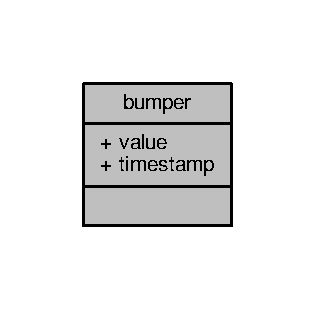
\includegraphics[width=151pt]{structbumper__coll__graph}
\end{center}
\end{figure}
\subsection*{Public Attributes}
\begin{DoxyCompactItemize}
\item 
\hypertarget{structbumper_a9fe58ba8100dac5c734c407545775300}{}int {\bfseries value}\label{structbumper_a9fe58ba8100dac5c734c407545775300}

\item 
\hypertarget{structbumper_a42639a9ad64823671784c081e527019e}{}std\+::string {\bfseries timestamp}\label{structbumper_a42639a9ad64823671784c081e527019e}

\end{DoxyCompactItemize}


The documentation for this struct was generated from the following file\+:\begin{DoxyCompactItemize}
\item 
/home/serge/\+Documents/\+Semester Project I\+N\+I/omnibot-\/lib/\+U\+S\+B\+\_\+robot/include/\hyperlink{_robot_listener_8h}{Robot\+Listener.\+h}\end{DoxyCompactItemize}

\hypertarget{classc_keyboard}{}\section{c\+Keyboard Class Reference}
\label{classc_keyboard}\index{c\+Keyboard@{c\+Keyboard}}


Manages the communication with an attached keyboard.  




{\ttfamily \#include $<$keyboard.\+h$>$}



Collaboration diagram for c\+Keyboard\+:
\nopagebreak
\begin{figure}[H]
\begin{center}
\leavevmode
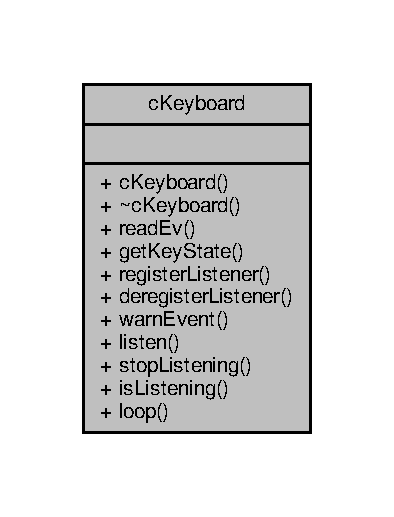
\includegraphics[width=189pt]{classc_keyboard__coll__graph}
\end{center}
\end{figure}
\subsection*{Public Member Functions}
\begin{DoxyCompactItemize}
\item 
\hypertarget{classc_keyboard_a2eeb7d5dc750a6ce73befe70705c1751}{}void \hyperlink{classc_keyboard_a2eeb7d5dc750a6ce73befe70705c1751}{read\+Ev} ()\label{classc_keyboard_a2eeb7d5dc750a6ce73befe70705c1751}

\begin{DoxyCompactList}\small\item\em gets a list of the pressed events from the keyboard. Pressing R \end{DoxyCompactList}\item 
\hypertarget{classc_keyboard_ac60892c71a46e7fc67a19ea75a4a394f}{}short {\bfseries get\+Key\+State} (short key)\label{classc_keyboard_ac60892c71a46e7fc67a19ea75a4a394f}

\item 
\hypertarget{classc_keyboard_a5be1e8b98017298f094ff418e18a5af9}{}void {\bfseries register\+Listener} (\hyperlink{class_keyboard_listener}{Keyboard\+Listener} $\ast$)\label{classc_keyboard_a5be1e8b98017298f094ff418e18a5af9}

\item 
\hypertarget{classc_keyboard_ad829c57a7662e5c6115d059c9739c9bf}{}void {\bfseries deregister\+Listener} (\hyperlink{class_keyboard_listener}{Keyboard\+Listener} $\ast$)\label{classc_keyboard_ad829c57a7662e5c6115d059c9739c9bf}

\item 
\hypertarget{classc_keyboard_a77b96029cc90ff2df970249570955024}{}void {\bfseries warn\+Event} (input\+\_\+event $\ast$)\label{classc_keyboard_a77b96029cc90ff2df970249570955024}

\item 
\hypertarget{classc_keyboard_a4facfef83ec4b2e66d114c3393ebd5e7}{}int \hyperlink{classc_keyboard_a4facfef83ec4b2e66d114c3393ebd5e7}{listen} ()\label{classc_keyboard_a4facfef83ec4b2e66d114c3393ebd5e7}

\begin{DoxyCompactList}\small\item\em Starts a new thread listening to the keyboard. \end{DoxyCompactList}\item 
\hypertarget{classc_keyboard_a6eb520c368e14d18fc417531c5c0b809}{}int \hyperlink{classc_keyboard_a6eb520c368e14d18fc417531c5c0b809}{stop\+Listening} ()\label{classc_keyboard_a6eb520c368e14d18fc417531c5c0b809}

\begin{DoxyCompactList}\small\item\em Stop listening and set m\+\_\+toggle\+Listening to false. \end{DoxyCompactList}\item 
\hypertarget{classc_keyboard_afb266be2c1e34f140d2a55f17f288af9}{}bool \hyperlink{classc_keyboard_afb266be2c1e34f140d2a55f17f288af9}{is\+Listening} ()\label{classc_keyboard_afb266be2c1e34f140d2a55f17f288af9}

\begin{DoxyCompactList}\small\item\em determines if an object is listening to the keyboard or not \end{DoxyCompactList}\end{DoxyCompactItemize}
\subsection*{Static Public Member Functions}
\begin{DoxyCompactItemize}
\item 
\hypertarget{classc_keyboard_ae02219e223b4074f844797d3707ed106}{}static void $\ast$ \hyperlink{classc_keyboard_ae02219e223b4074f844797d3707ed106}{loop} (void $\ast$obj)\label{classc_keyboard_ae02219e223b4074f844797d3707ed106}

\begin{DoxyCompactList}\small\item\em is executed in the new thread \end{DoxyCompactList}\end{DoxyCompactItemize}


\subsection{Detailed Description}
Manages the communication with an attached keyboard. 

\hyperlink{classc_keyboard}{c\+Keyboard} manages the communication with an attached keyboard. It is assumed that the attached keyboard has the expression \char`\"{}kbd\char`\"{} in its name. This class can detect key releases and key presses. 

The documentation for this class was generated from the following files\+:\begin{DoxyCompactItemize}
\item 
/home/serge/\+Documents/\+Semester Project I\+N\+I/omnibot-\/lib/\+U\+S\+B\+\_\+robot/include/\hyperlink{keyboard_8h}{keyboard.\+h}\item 
/home/serge/\+Documents/\+Semester Project I\+N\+I/omnibot-\/lib/\+U\+S\+B\+\_\+robot/src/\hyperlink{keyboard_8cpp}{keyboard.\+cpp}\end{DoxyCompactItemize}

\hypertarget{class_dumb_e_d_v_s4337_listener}{}\section{Dumb\+E\+D\+V\+S4337\+Listener Class Reference}
\label{class_dumb_e_d_v_s4337_listener}\index{Dumb\+E\+D\+V\+S4337\+Listener@{Dumb\+E\+D\+V\+S4337\+Listener}}


Inheritance diagram for Dumb\+E\+D\+V\+S4337\+Listener\+:
\nopagebreak
\begin{figure}[H]
\begin{center}
\leavevmode
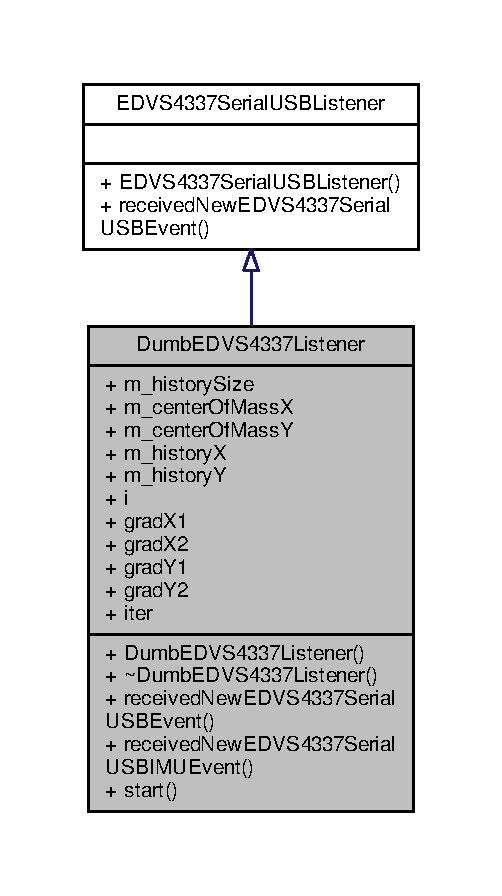
\includegraphics[width=241pt]{class_dumb_e_d_v_s4337_listener__inherit__graph}
\end{center}
\end{figure}


Collaboration diagram for Dumb\+E\+D\+V\+S4337\+Listener\+:
\nopagebreak
\begin{figure}[H]
\begin{center}
\leavevmode
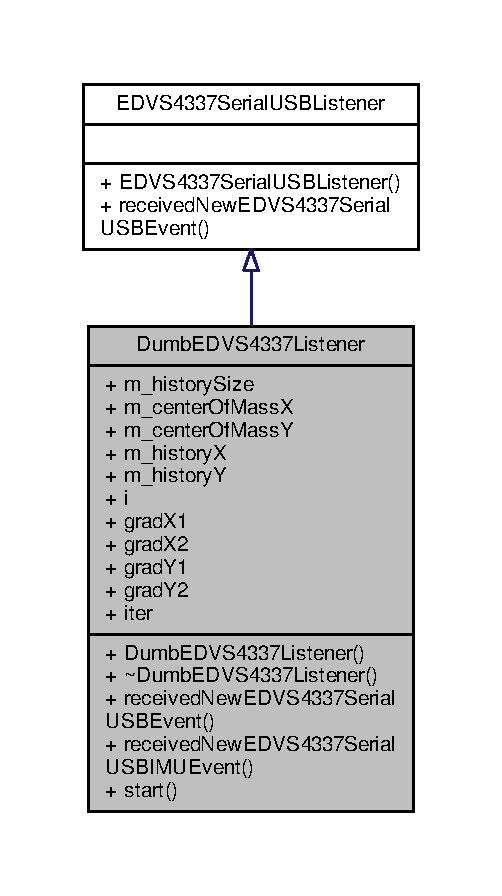
\includegraphics[width=241pt]{class_dumb_e_d_v_s4337_listener__coll__graph}
\end{center}
\end{figure}
\subsection*{Public Member Functions}
\begin{DoxyCompactItemize}
\item 
\hypertarget{class_dumb_e_d_v_s4337_listener_a2b41948d64b4d529e3a0e646e179e0e9}{}void \hyperlink{class_dumb_e_d_v_s4337_listener_a2b41948d64b4d529e3a0e646e179e0e9}{received\+New\+E\+D\+V\+S4337\+Serial\+U\+S\+B\+Event} (\hyperlink{struct_e_d_v_s4337_serial_u_s_b_event}{E\+D\+V\+S4337\+Serial\+U\+S\+B\+Event} \&e)\label{class_dumb_e_d_v_s4337_listener_a2b41948d64b4d529e3a0e646e179e0e9}

\begin{DoxyCompactList}\small\item\em Is invoked when a new event is parsed from the event stream. \end{DoxyCompactList}\item 
\hypertarget{class_dumb_e_d_v_s4337_listener_a6a04157d2fd293358261b9827842af38}{}void {\bfseries received\+New\+E\+D\+V\+S4337\+Serial\+U\+S\+B\+I\+M\+U\+Event} (\hyperlink{struct_e_d_v_s4337_serial_u_s_b_i_m_u_event}{E\+D\+V\+S4337\+Serial\+U\+S\+B\+I\+M\+U\+Event} \&e)\label{class_dumb_e_d_v_s4337_listener_a6a04157d2fd293358261b9827842af38}

\item 
\hypertarget{class_dumb_e_d_v_s4337_listener_a1c42cb95ff8b6588284aa52356e92954}{}void {\bfseries start} (void)\label{class_dumb_e_d_v_s4337_listener_a1c42cb95ff8b6588284aa52356e92954}

\end{DoxyCompactItemize}
\subsection*{Public Attributes}
\begin{DoxyCompactItemize}
\item 
\hypertarget{class_dumb_e_d_v_s4337_listener_aee50293da4b3013bb8aa5d592de9a4a4}{}unsigned int {\bfseries m\+\_\+history\+Size} = 20\label{class_dumb_e_d_v_s4337_listener_aee50293da4b3013bb8aa5d592de9a4a4}

\item 
\hypertarget{class_dumb_e_d_v_s4337_listener_a1de4cee6cabb6332989ae44ca8203c14}{}float {\bfseries m\+\_\+center\+Of\+Mass\+X} = 0.\+0\label{class_dumb_e_d_v_s4337_listener_a1de4cee6cabb6332989ae44ca8203c14}

\item 
\hypertarget{class_dumb_e_d_v_s4337_listener_aa17029e17a89e24dc6ae4fd014adc475}{}float {\bfseries m\+\_\+center\+Of\+Mass\+Y} = 0.\+0\label{class_dumb_e_d_v_s4337_listener_aa17029e17a89e24dc6ae4fd014adc475}

\item 
\hypertarget{class_dumb_e_d_v_s4337_listener_a49ef3387cc8252b7a21a4ec99da482ba}{}std\+::list$<$ float $>$ {\bfseries m\+\_\+history\+X}\label{class_dumb_e_d_v_s4337_listener_a49ef3387cc8252b7a21a4ec99da482ba}

\item 
\hypertarget{class_dumb_e_d_v_s4337_listener_a38238ca7cbcf8f755ac48f3ca2767fd8}{}std\+::list$<$ float $>$ {\bfseries m\+\_\+history\+Y}\label{class_dumb_e_d_v_s4337_listener_a38238ca7cbcf8f755ac48f3ca2767fd8}

\item 
\hypertarget{class_dumb_e_d_v_s4337_listener_a851e746950be6a518ee2c6aeb6364d9b}{}int {\bfseries i} = 0\label{class_dumb_e_d_v_s4337_listener_a851e746950be6a518ee2c6aeb6364d9b}

\item 
\hypertarget{class_dumb_e_d_v_s4337_listener_a03901730fcca782579637cc67951e534}{}float {\bfseries grad\+X1} = 0.\+0\label{class_dumb_e_d_v_s4337_listener_a03901730fcca782579637cc67951e534}

\item 
\hypertarget{class_dumb_e_d_v_s4337_listener_a7423ec5919dd8737bc20a3789a76cbe4}{}float {\bfseries grad\+X2} = 0.\+0\label{class_dumb_e_d_v_s4337_listener_a7423ec5919dd8737bc20a3789a76cbe4}

\item 
\hypertarget{class_dumb_e_d_v_s4337_listener_a78fe36a124c78dd2df87e519de15df35}{}float {\bfseries grad\+Y1} = 0.\+0\label{class_dumb_e_d_v_s4337_listener_a78fe36a124c78dd2df87e519de15df35}

\item 
\hypertarget{class_dumb_e_d_v_s4337_listener_aec34e1b8f90744fcd65e5b23809dcbda}{}float {\bfseries grad\+Y2} = 0.\+0\label{class_dumb_e_d_v_s4337_listener_aec34e1b8f90744fcd65e5b23809dcbda}

\item 
\hypertarget{class_dumb_e_d_v_s4337_listener_a7659b4a45469e721b663e5d05f56aa6e}{}int {\bfseries iter} = 0\label{class_dumb_e_d_v_s4337_listener_a7659b4a45469e721b663e5d05f56aa6e}

\end{DoxyCompactItemize}


The documentation for this class was generated from the following file\+:\begin{DoxyCompactItemize}
\item 
/home/serge/\+Documents/\+Semester Project I\+N\+I/omnibot-\/lib/\+U\+S\+B\+\_\+robot/include/dummy\+Listener.\+h\end{DoxyCompactItemize}

\hypertarget{class_e_d_v_s4337_serial_u_s_b}{}\section{E\+D\+V\+S4337\+Serial\+U\+S\+B Class Reference}
\label{class_e_d_v_s4337_serial_u_s_b}\index{E\+D\+V\+S4337\+Serial\+U\+S\+B@{E\+D\+V\+S4337\+Serial\+U\+S\+B}}


Class providing the necessary interfaces for communication and event streaming from the e\+D\+V\+S camera.  




{\ttfamily \#include $<$E\+B\+V\+\_\+\+E\+D\+V\+S4337\+Serial\+U\+S\+B.\+h$>$}



Collaboration diagram for E\+D\+V\+S4337\+Serial\+U\+S\+B\+:
\nopagebreak
\begin{figure}[H]
\begin{center}
\leavevmode
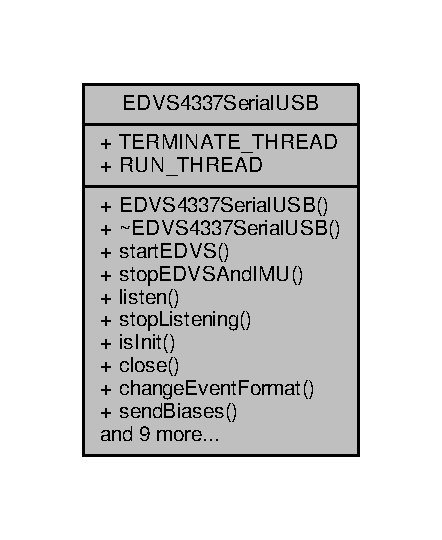
\includegraphics[width=212pt]{class_e_d_v_s4337_serial_u_s_b__coll__graph}
\end{center}
\end{figure}
\subsection*{Public Member Functions}
\begin{DoxyCompactItemize}
\item 
\hyperlink{class_e_d_v_s4337_serial_u_s_b_ab5f0ccc2d17dff50b7d282693db5f8e1}{E\+D\+V\+S4337\+Serial\+U\+S\+B} (int)
\begin{DoxyCompactList}\small\item\em constructor of the \hyperlink{class_e_d_v_s4337_serial_u_s_b}{E\+D\+V\+S4337\+Serial\+U\+S\+B} \end{DoxyCompactList}\item 
\hypertarget{class_e_d_v_s4337_serial_u_s_b_a69696b4657eb069eaa54f88a77e88cae}{}int \hyperlink{class_e_d_v_s4337_serial_u_s_b_a69696b4657eb069eaa54f88a77e88cae}{start\+E\+D\+V\+S} ()\label{class_e_d_v_s4337_serial_u_s_b_a69696b4657eb069eaa54f88a77e88cae}

\begin{DoxyCompactList}\small\item\em starts the e\+D\+V\+S by setting the necessary biases \end{DoxyCompactList}\item 
\hypertarget{class_e_d_v_s4337_serial_u_s_b_aa2d18776b99e4171f20e8814093bbe14}{}int \hyperlink{class_e_d_v_s4337_serial_u_s_b_aa2d18776b99e4171f20e8814093bbe14}{stop\+E\+D\+V\+S\+And\+I\+M\+U} ()\label{class_e_d_v_s4337_serial_u_s_b_aa2d18776b99e4171f20e8814093bbe14}

\begin{DoxyCompactList}\small\item\em stops the started e\+D\+V\+S and the I\+M\+U \end{DoxyCompactList}\item 
\hypertarget{class_e_d_v_s4337_serial_u_s_b_a944eee88553b63a6b0be88b0288e9199}{}int \hyperlink{class_e_d_v_s4337_serial_u_s_b_a944eee88553b63a6b0be88b0288e9199}{listen} ()\label{class_e_d_v_s4337_serial_u_s_b_a944eee88553b63a6b0be88b0288e9199}

\begin{DoxyCompactList}\small\item\em start listening to the events parsed from the event stream \end{DoxyCompactList}\item 
\hypertarget{class_e_d_v_s4337_serial_u_s_b_ae219efb04db44707bf67928f986969d1}{}int \hyperlink{class_e_d_v_s4337_serial_u_s_b_ae219efb04db44707bf67928f986969d1}{stop\+Listening} ()\label{class_e_d_v_s4337_serial_u_s_b_ae219efb04db44707bf67928f986969d1}

\begin{DoxyCompactList}\small\item\em stop listening to the events parsed from the event stream \end{DoxyCompactList}\item 
int \hyperlink{class_e_d_v_s4337_serial_u_s_b_aebb4071c2c8b81771460e8381016c3a0}{is\+Init} ()
\begin{DoxyCompactList}\small\item\em checks if the camera is correctly initialized \end{DoxyCompactList}\item 
\hypertarget{class_e_d_v_s4337_serial_u_s_b_a3d1cfe0acb88ab31523477519df51f17}{}int \hyperlink{class_e_d_v_s4337_serial_u_s_b_a3d1cfe0acb88ab31523477519df51f17}{close} ()\label{class_e_d_v_s4337_serial_u_s_b_a3d1cfe0acb88ab31523477519df51f17}

\begin{DoxyCompactList}\small\item\em closes the serial Port to the e\+D\+V\+S camera \end{DoxyCompactList}\item 
int \hyperlink{class_e_d_v_s4337_serial_u_s_b_a34bbef40b445d99ea326fda021235079}{change\+Event\+Format} (\hyperlink{_e_b_v___e_d_v_s4337_serial_u_s_b_8h_a2b0bc356728b430ea3809f44d9be46c1}{Event\+Format})
\begin{DoxyCompactList}\small\item\em changes the event format of the events \end{DoxyCompactList}\item 
int \hyperlink{class_e_d_v_s4337_serial_u_s_b_af09e53dfaa5b511faf6992e47aa8b970}{send\+Biases} (\hyperlink{struct_e_d_v_s4337_serial_u_s_b_biases}{E\+D\+V\+S4337\+Serial\+U\+S\+B\+Biases} b=\hyperlink{struct_e_d_v_s4337_serial_u_s_b_biases}{E\+D\+V\+S4337\+Serial\+U\+S\+B\+Biases}())
\begin{DoxyCompactList}\small\item\em send biases to the camera \end{DoxyCompactList}\item 
\hypertarget{class_e_d_v_s4337_serial_u_s_b_a327ddd8ac04b7e69ba01bd90ae49f040}{}\hyperlink{struct_e_d_v_s4337_serial_u_s_b_biases}{E\+D\+V\+S4337\+Serial\+U\+S\+B\+Biases} \hyperlink{class_e_d_v_s4337_serial_u_s_b_a327ddd8ac04b7e69ba01bd90ae49f040}{get\+Biases} ()\label{class_e_d_v_s4337_serial_u_s_b_a327ddd8ac04b7e69ba01bd90ae49f040}

\begin{DoxyCompactList}\small\item\em get the current biases \end{DoxyCompactList}\item 
\hypertarget{class_e_d_v_s4337_serial_u_s_b_a205afab634036c014dcb84184746635c}{}void \hyperlink{class_e_d_v_s4337_serial_u_s_b_a205afab634036c014dcb84184746635c}{register\+Listener} (\hyperlink{class_e_d_v_s4337_serial_u_s_b_listener}{E\+D\+V\+S4337\+Serial\+U\+S\+B\+Listener} $\ast$listener)\label{class_e_d_v_s4337_serial_u_s_b_a205afab634036c014dcb84184746635c}

\begin{DoxyCompactList}\small\item\em Register an event listener. \end{DoxyCompactList}\item 
void \hyperlink{class_e_d_v_s4337_serial_u_s_b_a327a91b0d54282de0ae8fdcc47e15b0a}{deregister\+Listener} (\hyperlink{class_e_d_v_s4337_serial_u_s_b_listener}{E\+D\+V\+S4337\+Serial\+U\+S\+B\+Listener} $\ast$listener)
\begin{DoxyCompactList}\small\item\em deregister a specific event listener. \end{DoxyCompactList}\item 
void \hyperlink{class_e_d_v_s4337_serial_u_s_b_a78e3c01f241b7e40debd7be4556d69c3}{register\+I\+M\+U\+Listener} (\hyperlink{class_e_d_v_s4337_serial_u_s_b_i_m_u_listener}{E\+D\+V\+S4337\+Serial\+U\+S\+B\+I\+M\+U\+Listener} $\ast$listener)
\item 
\hypertarget{class_e_d_v_s4337_serial_u_s_b_a4f46c52151f14a417c3051554e6d55c9}{}void {\bfseries deregister\+I\+M\+U\+Listener} (\hyperlink{class_e_d_v_s4337_serial_u_s_b_i_m_u_listener}{E\+D\+V\+S4337\+Serial\+U\+S\+B\+I\+M\+U\+Listener} $\ast$listener)\label{class_e_d_v_s4337_serial_u_s_b_a4f46c52151f14a417c3051554e6d55c9}

\item 
\hypertarget{class_e_d_v_s4337_serial_u_s_b_abddef8a14c7460309a50ab8087c96c35}{}void \hyperlink{class_e_d_v_s4337_serial_u_s_b_abddef8a14c7460309a50ab8087c96c35}{warn\+Event} (std\+::vector$<$ \hyperlink{struct_e_d_v_s4337_serial_u_s_b_event}{E\+D\+V\+S4337\+Serial\+U\+S\+B\+Event} $>$ \&events)\label{class_e_d_v_s4337_serial_u_s_b_abddef8a14c7460309a50ab8087c96c35}

\begin{DoxyCompactList}\small\item\em Notify all the event listeners that an event as occured. \end{DoxyCompactList}\item 
\hypertarget{class_e_d_v_s4337_serial_u_s_b_a8428d013f20a418abd24f48b89f0b128}{}void \hyperlink{class_e_d_v_s4337_serial_u_s_b_a8428d013f20a418abd24f48b89f0b128}{warn\+I\+M\+U\+Event} (std\+::vector$<$ \hyperlink{struct_e_d_v_s4337_serial_u_s_b_i_m_u_event}{E\+D\+V\+S4337\+Serial\+U\+S\+B\+I\+M\+U\+Event} $>$ \&events)\label{class_e_d_v_s4337_serial_u_s_b_a8428d013f20a418abd24f48b89f0b128}

\begin{DoxyCompactList}\small\item\em Notify all the I\+M\+U event listeners that an event as occured. \end{DoxyCompactList}\item 
\hypertarget{class_e_d_v_s4337_serial_u_s_b_aac0296a78f69948dbf43611425998e23}{}void \hyperlink{class_e_d_v_s4337_serial_u_s_b_aac0296a78f69948dbf43611425998e23}{start\+I\+M\+U} (E\+D\+V\+S4337\+Serial\+U\+S\+B\+I\+M\+U\+Event\+::\+I\+M\+U\+Type, int)\label{class_e_d_v_s4337_serial_u_s_b_aac0296a78f69948dbf43611425998e23}

\begin{DoxyCompactList}\small\item\em starts the I\+M\+U by sending the necessary commands \end{DoxyCompactList}\item 
\hypertarget{class_e_d_v_s4337_serial_u_s_b_ad7cd708dd39311ac007d30927e335a5b}{}void \hyperlink{class_e_d_v_s4337_serial_u_s_b_ad7cd708dd39311ac007d30927e335a5b}{stop\+I\+M\+U} (E\+D\+V\+S4337\+Serial\+U\+S\+B\+I\+M\+U\+Event\+::\+I\+M\+U\+Type)\label{class_e_d_v_s4337_serial_u_s_b_ad7cd708dd39311ac007d30927e335a5b}

\begin{DoxyCompactList}\small\item\em starts the I\+M\+U by sending the necessary commands \end{DoxyCompactList}\end{DoxyCompactItemize}
\subsection*{Static Public Attributes}
\begin{DoxyCompactItemize}
\item 
\hypertarget{class_e_d_v_s4337_serial_u_s_b_a97c4bc902063509a0934e0aa07a3a0c2}{}static const int \hyperlink{class_e_d_v_s4337_serial_u_s_b_a97c4bc902063509a0934e0aa07a3a0c2}{T\+E\+R\+M\+I\+N\+A\+T\+E\+\_\+\+T\+H\+R\+E\+A\+D} = -\/1\label{class_e_d_v_s4337_serial_u_s_b_a97c4bc902063509a0934e0aa07a3a0c2}

\begin{DoxyCompactList}\small\item\em Flag indicating when to stop the reading thread. \end{DoxyCompactList}\item 
\hypertarget{class_e_d_v_s4337_serial_u_s_b_a89f3d76801ef1b50641ecb6cd5c7e113}{}static const int \hyperlink{class_e_d_v_s4337_serial_u_s_b_a89f3d76801ef1b50641ecb6cd5c7e113}{R\+U\+N\+\_\+\+T\+H\+R\+E\+A\+D} = 1\label{class_e_d_v_s4337_serial_u_s_b_a89f3d76801ef1b50641ecb6cd5c7e113}

\begin{DoxyCompactList}\small\item\em Flag indicating when to start the reading thread. \end{DoxyCompactList}\end{DoxyCompactItemize}


\subsection{Detailed Description}
Class providing the necessary interfaces for communication and event streaming from the e\+D\+V\+S camera. 

The e\+D\+V\+S camera is fitted with a F\+T\+D\+I chip, such that the camera can be opened and handeled like a serial port, despite the connection is established via U\+S\+B. 

\subsection{Constructor \& Destructor Documentation}
\hypertarget{class_e_d_v_s4337_serial_u_s_b_ab5f0ccc2d17dff50b7d282693db5f8e1}{}\index{E\+D\+V\+S4337\+Serial\+U\+S\+B@{E\+D\+V\+S4337\+Serial\+U\+S\+B}!E\+D\+V\+S4337\+Serial\+U\+S\+B@{E\+D\+V\+S4337\+Serial\+U\+S\+B}}
\index{E\+D\+V\+S4337\+Serial\+U\+S\+B@{E\+D\+V\+S4337\+Serial\+U\+S\+B}!E\+D\+V\+S4337\+Serial\+U\+S\+B@{E\+D\+V\+S4337\+Serial\+U\+S\+B}}
\subsubsection[{E\+D\+V\+S4337\+Serial\+U\+S\+B}]{\setlength{\rightskip}{0pt plus 5cm}E\+D\+V\+S4337\+Serial\+U\+S\+B\+::\+E\+D\+V\+S4337\+Serial\+U\+S\+B (
\begin{DoxyParamCaption}
\item[{int}]{file\+Descriptor}
\end{DoxyParamCaption}
)}\label{class_e_d_v_s4337_serial_u_s_b_ab5f0ccc2d17dff50b7d282693db5f8e1}


constructor of the \hyperlink{class_e_d_v_s4337_serial_u_s_b}{E\+D\+V\+S4337\+Serial\+U\+S\+B} 


\begin{DoxyParams}{Parameters}
{\em int} & valid file descriptor to the e\+D\+V\+S camera \\
\hline
\end{DoxyParams}


\subsection{Member Function Documentation}
\hypertarget{class_e_d_v_s4337_serial_u_s_b_a34bbef40b445d99ea326fda021235079}{}\index{E\+D\+V\+S4337\+Serial\+U\+S\+B@{E\+D\+V\+S4337\+Serial\+U\+S\+B}!change\+Event\+Format@{change\+Event\+Format}}
\index{change\+Event\+Format@{change\+Event\+Format}!E\+D\+V\+S4337\+Serial\+U\+S\+B@{E\+D\+V\+S4337\+Serial\+U\+S\+B}}
\subsubsection[{change\+Event\+Format}]{\setlength{\rightskip}{0pt plus 5cm}int E\+D\+V\+S4337\+Serial\+U\+S\+B\+::change\+Event\+Format (
\begin{DoxyParamCaption}
\item[{{\bf Event\+Format}}]{fmt}
\end{DoxyParamCaption}
)}\label{class_e_d_v_s4337_serial_u_s_b_a34bbef40b445d99ea326fda021235079}


changes the event format of the events 

\begin{DoxySeeAlso}{See also}
\hyperlink{_e_b_v___e_d_v_s4337_serial_u_s_b_8h_a2b0bc356728b430ea3809f44d9be46c1}{Event\+Format} for the supported events 
\end{DoxySeeAlso}
\hypertarget{class_e_d_v_s4337_serial_u_s_b_a327a91b0d54282de0ae8fdcc47e15b0a}{}\index{E\+D\+V\+S4337\+Serial\+U\+S\+B@{E\+D\+V\+S4337\+Serial\+U\+S\+B}!deregister\+Listener@{deregister\+Listener}}
\index{deregister\+Listener@{deregister\+Listener}!E\+D\+V\+S4337\+Serial\+U\+S\+B@{E\+D\+V\+S4337\+Serial\+U\+S\+B}}
\subsubsection[{deregister\+Listener}]{\setlength{\rightskip}{0pt plus 5cm}void E\+D\+V\+S4337\+Serial\+U\+S\+B\+::deregister\+Listener (
\begin{DoxyParamCaption}
\item[{{\bf E\+D\+V\+S4337\+Serial\+U\+S\+B\+Listener} $\ast$}]{listener}
\end{DoxyParamCaption}
)}\label{class_e_d_v_s4337_serial_u_s_b_a327a91b0d54282de0ae8fdcc47e15b0a}


deregister a specific event listener. 


\begin{DoxyParams}{Parameters}
{\em listener} & specifies the listener to be removed \\
\hline
\end{DoxyParams}
\hypertarget{class_e_d_v_s4337_serial_u_s_b_aebb4071c2c8b81771460e8381016c3a0}{}\index{E\+D\+V\+S4337\+Serial\+U\+S\+B@{E\+D\+V\+S4337\+Serial\+U\+S\+B}!is\+Init@{is\+Init}}
\index{is\+Init@{is\+Init}!E\+D\+V\+S4337\+Serial\+U\+S\+B@{E\+D\+V\+S4337\+Serial\+U\+S\+B}}
\subsubsection[{is\+Init}]{\setlength{\rightskip}{0pt plus 5cm}int E\+D\+V\+S4337\+Serial\+U\+S\+B\+::is\+Init (
\begin{DoxyParamCaption}
{}
\end{DoxyParamCaption}
)}\label{class_e_d_v_s4337_serial_u_s_b_aebb4071c2c8b81771460e8381016c3a0}


checks if the camera is correctly initialized 

\begin{DoxyReturn}{Returns}
1 if the camera has been corectly initialized, else -\/1 
\end{DoxyReturn}
\hypertarget{class_e_d_v_s4337_serial_u_s_b_a78e3c01f241b7e40debd7be4556d69c3}{}\index{E\+D\+V\+S4337\+Serial\+U\+S\+B@{E\+D\+V\+S4337\+Serial\+U\+S\+B}!register\+I\+M\+U\+Listener@{register\+I\+M\+U\+Listener}}
\index{register\+I\+M\+U\+Listener@{register\+I\+M\+U\+Listener}!E\+D\+V\+S4337\+Serial\+U\+S\+B@{E\+D\+V\+S4337\+Serial\+U\+S\+B}}
\subsubsection[{register\+I\+M\+U\+Listener}]{\setlength{\rightskip}{0pt plus 5cm}void E\+D\+V\+S4337\+Serial\+U\+S\+B\+::register\+I\+M\+U\+Listener (
\begin{DoxyParamCaption}
\item[{{\bf E\+D\+V\+S4337\+Serial\+U\+S\+B\+I\+M\+U\+Listener} $\ast$}]{listener}
\end{DoxyParamCaption}
)}\label{class_e_d_v_s4337_serial_u_s_b_a78e3c01f241b7e40debd7be4556d69c3}
Register an I\+M\+U event listener deregister a specific I\+M\+U event listener.


\begin{DoxyParams}{Parameters}
{\em listener} & specifies the listener to be removed \\
\hline
\end{DoxyParams}
\hypertarget{class_e_d_v_s4337_serial_u_s_b_af09e53dfaa5b511faf6992e47aa8b970}{}\index{E\+D\+V\+S4337\+Serial\+U\+S\+B@{E\+D\+V\+S4337\+Serial\+U\+S\+B}!send\+Biases@{send\+Biases}}
\index{send\+Biases@{send\+Biases}!E\+D\+V\+S4337\+Serial\+U\+S\+B@{E\+D\+V\+S4337\+Serial\+U\+S\+B}}
\subsubsection[{send\+Biases}]{\setlength{\rightskip}{0pt plus 5cm}int E\+D\+V\+S4337\+Serial\+U\+S\+B\+::send\+Biases (
\begin{DoxyParamCaption}
\item[{{\bf E\+D\+V\+S4337\+Serial\+U\+S\+B\+Biases}}]{b = {\ttfamily {\bf E\+D\+V\+S4337\+Serial\+U\+S\+B\+Biases}()}}
\end{DoxyParamCaption}
)}\label{class_e_d_v_s4337_serial_u_s_b_af09e53dfaa5b511faf6992e47aa8b970}


send biases to the camera 


\begin{DoxyParams}{Parameters}
{\em \hyperlink{struct_e_d_v_s4337_serial_u_s_b_biases}{E\+D\+V\+S4337\+Serial\+U\+S\+B\+Biases}} & b is struct with the values of the biases to be set. \\
\hline
\end{DoxyParams}
\begin{DoxySeeAlso}{See also}
\hyperlink{_e_b_v___e_d_v_s4337_serial_u_s_b_8h_a0580b5f9d6ec67f7bb47b4f52cff0cfd}{biases\+\_\+t} for all the biases that can be manipulated 
\end{DoxySeeAlso}


The documentation for this class was generated from the following files\+:\begin{DoxyCompactItemize}
\item 
/home/serge/\+Documents/\+Semester Project I\+N\+I/omnibot-\/lib/\+U\+S\+B\+\_\+robot/include/\hyperlink{_e_b_v___e_d_v_s4337_serial_u_s_b_8h}{E\+B\+V\+\_\+\+E\+D\+V\+S4337\+Serial\+U\+S\+B.\+h}\item 
/home/serge/\+Documents/\+Semester Project I\+N\+I/omnibot-\/lib/\+U\+S\+B\+\_\+robot/src/E\+B\+V\+\_\+\+E\+D\+V\+S4337\+Serial\+U\+S\+B.\+cpp\end{DoxyCompactItemize}

\hypertarget{struct_e_d_v_s4337_serial_u_s_b_args}{}\section{E\+D\+V\+S4337\+Serial\+U\+S\+B\+Args Struct Reference}
\label{struct_e_d_v_s4337_serial_u_s_b_args}\index{E\+D\+V\+S4337\+Serial\+U\+S\+B\+Args@{E\+D\+V\+S4337\+Serial\+U\+S\+B\+Args}}


encapsulates the necessary arguments to start reading from the serial port in a new Threading  




{\ttfamily \#include $<$E\+B\+V\+\_\+\+E\+D\+V\+S4337\+Serial\+U\+S\+B.\+h$>$}



Collaboration diagram for E\+D\+V\+S4337\+Serial\+U\+S\+B\+Args\+:
\nopagebreak
\begin{figure}[H]
\begin{center}
\leavevmode
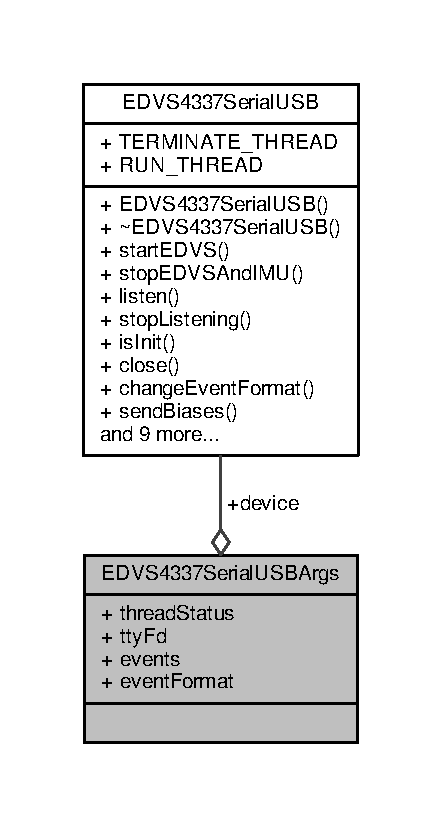
\includegraphics[width=212pt]{struct_e_d_v_s4337_serial_u_s_b_args__coll__graph}
\end{center}
\end{figure}
\subsection*{Public Attributes}
\begin{DoxyCompactItemize}
\item 
\hypertarget{struct_e_d_v_s4337_serial_u_s_b_args_a817d919c3ff1a29b968011757857a27c}{}\hyperlink{class_e_d_v_s4337_serial_u_s_b}{E\+D\+V\+S4337\+Serial\+U\+S\+B} $\ast$ {\bfseries device}\label{struct_e_d_v_s4337_serial_u_s_b_args_a817d919c3ff1a29b968011757857a27c}

\item 
\hypertarget{struct_e_d_v_s4337_serial_u_s_b_args_aae8bd4bb2c628a16cbed119fd405406c}{}int $\ast$ {\bfseries thread\+Status}\label{struct_e_d_v_s4337_serial_u_s_b_args_aae8bd4bb2c628a16cbed119fd405406c}

\item 
\hypertarget{struct_e_d_v_s4337_serial_u_s_b_args_a351b7fc5f36a61597cc36139e4cabf81}{}int $\ast$ {\bfseries tty\+Fd}\label{struct_e_d_v_s4337_serial_u_s_b_args_a351b7fc5f36a61597cc36139e4cabf81}

\item 
\hypertarget{struct_e_d_v_s4337_serial_u_s_b_args_aaef561e6facb2a8f495d509f262b3e0b}{}std\+::list$<$ \hyperlink{struct_e_d_v_s4337_serial_u_s_b_event}{E\+D\+V\+S4337\+Serial\+U\+S\+B\+Event} $>$ $\ast$ {\bfseries events}\label{struct_e_d_v_s4337_serial_u_s_b_args_aaef561e6facb2a8f495d509f262b3e0b}

\item 
\hypertarget{struct_e_d_v_s4337_serial_u_s_b_args_a4f446a992e08e47a9ef9c6ebf2199bcc}{}\hyperlink{_e_b_v___e_d_v_s4337_serial_u_s_b_8h_a2b0bc356728b430ea3809f44d9be46c1}{Event\+Format} $\ast$ {\bfseries event\+Format}\label{struct_e_d_v_s4337_serial_u_s_b_args_a4f446a992e08e47a9ef9c6ebf2199bcc}

\end{DoxyCompactItemize}


\subsection{Detailed Description}
encapsulates the necessary arguments to start reading from the serial port in a new Threading 

\begin{DoxySeeAlso}{See also}
read\+Thread\+E\+D\+V\+S4337 
\end{DoxySeeAlso}


The documentation for this struct was generated from the following file\+:\begin{DoxyCompactItemize}
\item 
/home/serge/\+Documents/\+Semester Project I\+N\+I/omnibot-\/lib/\+U\+S\+B\+\_\+robot/include/\hyperlink{_e_b_v___e_d_v_s4337_serial_u_s_b_8h}{E\+B\+V\+\_\+\+E\+D\+V\+S4337\+Serial\+U\+S\+B.\+h}\end{DoxyCompactItemize}

\hypertarget{struct_e_d_v_s4337_serial_u_s_b_biases}{}\section{E\+D\+V\+S4337\+Serial\+U\+S\+B\+Biases Struct Reference}
\label{struct_e_d_v_s4337_serial_u_s_b_biases}\index{E\+D\+V\+S4337\+Serial\+U\+S\+B\+Biases@{E\+D\+V\+S4337\+Serial\+U\+S\+B\+Biases}}


encapsulates the values for the biases and stores them in an array with the help of the biases\+\_\+t enum for better readability.  




{\ttfamily \#include $<$E\+B\+V\+\_\+\+E\+D\+V\+S4337\+Serial\+U\+S\+B.\+h$>$}



Collaboration diagram for E\+D\+V\+S4337\+Serial\+U\+S\+B\+Biases\+:
\nopagebreak
\begin{figure}[H]
\begin{center}
\leavevmode
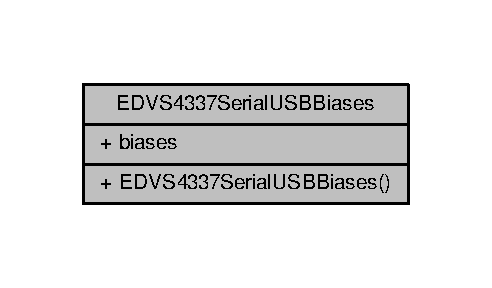
\includegraphics[width=236pt]{struct_e_d_v_s4337_serial_u_s_b_biases__coll__graph}
\end{center}
\end{figure}
\subsection*{Public Attributes}
\begin{DoxyCompactItemize}
\item 
\hypertarget{struct_e_d_v_s4337_serial_u_s_b_biases_a35f86bae016e35fcd7859e0276cab60b}{}int \hyperlink{struct_e_d_v_s4337_serial_u_s_b_biases_a35f86bae016e35fcd7859e0276cab60b}{biases} \mbox{[}12\mbox{]}\label{struct_e_d_v_s4337_serial_u_s_b_biases_a35f86bae016e35fcd7859e0276cab60b}

\begin{DoxyCompactList}\small\item\em array with the biases, can be convientently accessed with the biases\+\_\+t enum. \end{DoxyCompactList}\end{DoxyCompactItemize}


\subsection{Detailed Description}
encapsulates the values for the biases and stores them in an array with the help of the biases\+\_\+t enum for better readability. 

\begin{DoxySeeAlso}{See also}
\hyperlink{_e_b_v___e_d_v_s4337_serial_u_s_b_8h_a0580b5f9d6ec67f7bb47b4f52cff0cfd}{biases\+\_\+t} 
\end{DoxySeeAlso}


The documentation for this struct was generated from the following file\+:\begin{DoxyCompactItemize}
\item 
/home/serge/\+Documents/\+Semester Project I\+N\+I/omnibot-\/lib/\+U\+S\+B\+\_\+robot/include/\hyperlink{_e_b_v___e_d_v_s4337_serial_u_s_b_8h}{E\+B\+V\+\_\+\+E\+D\+V\+S4337\+Serial\+U\+S\+B.\+h}\end{DoxyCompactItemize}

\hypertarget{struct_e_d_v_s4337_serial_u_s_b_event}{}\section{E\+D\+V\+S4337\+Serial\+U\+S\+B\+Event Class Reference}
\label{struct_e_d_v_s4337_serial_u_s_b_event}\index{E\+D\+V\+S4337\+Serial\+U\+S\+B\+Event@{E\+D\+V\+S4337\+Serial\+U\+S\+B\+Event}}


encapsulates the camera events parsed from the event stream coming from the e\+D\+V\+S.  




{\ttfamily \#include $<$E\+B\+V\+\_\+\+E\+D\+V\+S4337\+Serial\+U\+S\+B.\+h$>$}



Collaboration diagram for E\+D\+V\+S4337\+Serial\+U\+S\+B\+Event\+:
\nopagebreak
\begin{figure}[H]
\begin{center}
\leavevmode
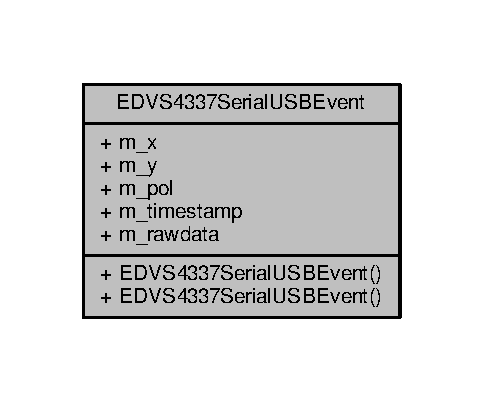
\includegraphics[width=232pt]{struct_e_d_v_s4337_serial_u_s_b_event__coll__graph}
\end{center}
\end{figure}
\subsection*{Public Member Functions}
\begin{DoxyCompactItemize}
\item 
\hypertarget{struct_e_d_v_s4337_serial_u_s_b_event_af943a6148b48468f291cf35ade44bcea}{}{\bfseries E\+D\+V\+S4337\+Serial\+U\+S\+B\+Event} (const unsigned int x, const unsigned int y, const int pol, const unsigned long timestamp)\label{struct_e_d_v_s4337_serial_u_s_b_event_af943a6148b48468f291cf35ade44bcea}

\end{DoxyCompactItemize}
\subsection*{Public Attributes}
\begin{DoxyCompactItemize}
\item 
\hypertarget{struct_e_d_v_s4337_serial_u_s_b_event_a8f1a90c369140ba5abf9a6d0ef309e12}{}unsigned int \hyperlink{struct_e_d_v_s4337_serial_u_s_b_event_a8f1a90c369140ba5abf9a6d0ef309e12}{m\+\_\+x}\label{struct_e_d_v_s4337_serial_u_s_b_event_a8f1a90c369140ba5abf9a6d0ef309e12}

\begin{DoxyCompactList}\small\item\em x position of the pixel that fired \end{DoxyCompactList}\item 
\hypertarget{struct_e_d_v_s4337_serial_u_s_b_event_a397b869776253fac7c2b2ac59b8b3cbe}{}unsigned int \hyperlink{struct_e_d_v_s4337_serial_u_s_b_event_a397b869776253fac7c2b2ac59b8b3cbe}{m\+\_\+y}\label{struct_e_d_v_s4337_serial_u_s_b_event_a397b869776253fac7c2b2ac59b8b3cbe}

\begin{DoxyCompactList}\small\item\em y position of the pixel that fired \end{DoxyCompactList}\item 
\hypertarget{struct_e_d_v_s4337_serial_u_s_b_event_ad7f69be52ec9ba031c5ee2f89a881f65}{}int \hyperlink{struct_e_d_v_s4337_serial_u_s_b_event_ad7f69be52ec9ba031c5ee2f89a881f65}{m\+\_\+pol}\label{struct_e_d_v_s4337_serial_u_s_b_event_ad7f69be52ec9ba031c5ee2f89a881f65}

\begin{DoxyCompactList}\small\item\em polarity of the pixel that fired, assumes the values 0 or 1 \end{DoxyCompactList}\item 
\hypertarget{struct_e_d_v_s4337_serial_u_s_b_event_abfbb4fa439b43c69638a9f0a9d596afe}{}unsigned long \hyperlink{struct_e_d_v_s4337_serial_u_s_b_event_abfbb4fa439b43c69638a9f0a9d596afe}{m\+\_\+timestamp}\label{struct_e_d_v_s4337_serial_u_s_b_event_abfbb4fa439b43c69638a9f0a9d596afe}

\begin{DoxyCompactList}\small\item\em timestamp set by the e\+D\+V\+S camera \end{DoxyCompactList}\item 
\hypertarget{struct_e_d_v_s4337_serial_u_s_b_event_af3cef2482b5d7beb1d6297b27db7aa2d}{}char \hyperlink{struct_e_d_v_s4337_serial_u_s_b_event_af3cef2482b5d7beb1d6297b27db7aa2d}{m\+\_\+rawdata} \mbox{[}8\mbox{]}\label{struct_e_d_v_s4337_serial_u_s_b_event_af3cef2482b5d7beb1d6297b27db7aa2d}

\begin{DoxyCompactList}\small\item\em raw data of the event as from the e\+D\+V\+S event stream \end{DoxyCompactList}\end{DoxyCompactItemize}


\subsection{Detailed Description}
encapsulates the camera events parsed from the event stream coming from the e\+D\+V\+S. 

The documentation for this class was generated from the following file\+:\begin{DoxyCompactItemize}
\item 
/home/serge/\+Documents/\+Semester Project I\+N\+I/omnibot-\/lib/\+U\+S\+B\+\_\+robot/include/\hyperlink{_e_b_v___e_d_v_s4337_serial_u_s_b_8h}{E\+B\+V\+\_\+\+E\+D\+V\+S4337\+Serial\+U\+S\+B.\+h}\end{DoxyCompactItemize}

\hypertarget{struct_e_d_v_s4337_serial_u_s_b_i_m_u_event}{}\section{E\+D\+V\+S4337\+Serial\+U\+S\+B\+I\+M\+U\+Event Class Reference}
\label{struct_e_d_v_s4337_serial_u_s_b_i_m_u_event}\index{E\+D\+V\+S4337\+Serial\+U\+S\+B\+I\+M\+U\+Event@{E\+D\+V\+S4337\+Serial\+U\+S\+B\+I\+M\+U\+Event}}


encapsulates the I\+M\+U events parsed from the event stream coming from the e\+D\+V\+S.  




{\ttfamily \#include $<$E\+B\+V\+\_\+\+E\+D\+V\+S4337\+Serial\+U\+S\+B.\+h$>$}



Collaboration diagram for E\+D\+V\+S4337\+Serial\+U\+S\+B\+I\+M\+U\+Event\+:
\nopagebreak
\begin{figure}[H]
\begin{center}
\leavevmode
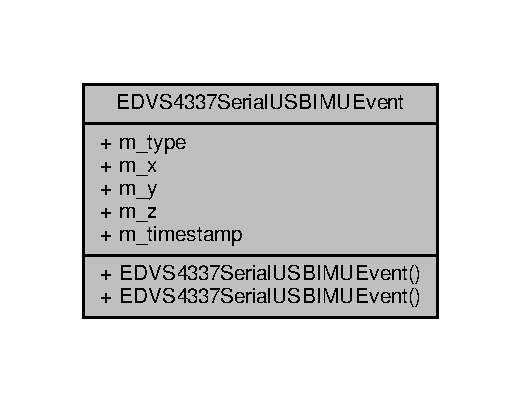
\includegraphics[width=250pt]{struct_e_d_v_s4337_serial_u_s_b_i_m_u_event__coll__graph}
\end{center}
\end{figure}
\subsection*{Public Types}
\begin{DoxyCompactItemize}
\item 
\hypertarget{struct_e_d_v_s4337_serial_u_s_b_i_m_u_event_a3c56f5e905756730da552d17d107455c}{}enum {\bfseries I\+M\+U\+Type} \{ {\bfseries I\+M\+U\+\_\+\+C\+O\+M\+P\+A\+S\+S}, 
{\bfseries I\+M\+U\+\_\+\+A\+C\+C\+E\+L\+E\+R\+O\+M\+E\+T\+E\+R}, 
{\bfseries I\+M\+U\+\_\+\+G\+Y\+R\+O}, 
{\bfseries I\+M\+U\+\_\+\+U\+N\+D\+E\+F\+I\+N\+E\+D}
 \}\label{struct_e_d_v_s4337_serial_u_s_b_i_m_u_event_a3c56f5e905756730da552d17d107455c}

\end{DoxyCompactItemize}
\subsection*{Public Member Functions}
\begin{DoxyCompactItemize}
\item 
\hypertarget{struct_e_d_v_s4337_serial_u_s_b_i_m_u_event_a07c079c07eb2d0c70089cc3edbd7a168}{}{\bfseries E\+D\+V\+S4337\+Serial\+U\+S\+B\+I\+M\+U\+Event} (I\+M\+U\+Type type, int x, int y, int z, unsigned int timestamp)\label{struct_e_d_v_s4337_serial_u_s_b_i_m_u_event_a07c079c07eb2d0c70089cc3edbd7a168}

\end{DoxyCompactItemize}
\subsection*{Public Attributes}
\begin{DoxyCompactItemize}
\item 
\hypertarget{struct_e_d_v_s4337_serial_u_s_b_i_m_u_event_aa8edf2c7de82e894e6fc814b5390510f}{}I\+M\+U\+Type {\bfseries m\+\_\+type}\label{struct_e_d_v_s4337_serial_u_s_b_i_m_u_event_aa8edf2c7de82e894e6fc814b5390510f}

\item 
\hypertarget{struct_e_d_v_s4337_serial_u_s_b_i_m_u_event_abbb34d1ed175541706b5ec8ec26da02d}{}int {\bfseries m\+\_\+x}\label{struct_e_d_v_s4337_serial_u_s_b_i_m_u_event_abbb34d1ed175541706b5ec8ec26da02d}

\item 
\hypertarget{struct_e_d_v_s4337_serial_u_s_b_i_m_u_event_a879673f328146dc4704e086a15d3be9c}{}int {\bfseries m\+\_\+y}\label{struct_e_d_v_s4337_serial_u_s_b_i_m_u_event_a879673f328146dc4704e086a15d3be9c}

\item 
\hypertarget{struct_e_d_v_s4337_serial_u_s_b_i_m_u_event_abf017343cf4fdce2385b84236eb21809}{}int {\bfseries m\+\_\+z}\label{struct_e_d_v_s4337_serial_u_s_b_i_m_u_event_abf017343cf4fdce2385b84236eb21809}

\item 
\hypertarget{struct_e_d_v_s4337_serial_u_s_b_i_m_u_event_af3db6c4af22b5a3b224d1325ba6ea5a0}{}unsigned int {\bfseries m\+\_\+timestamp}\label{struct_e_d_v_s4337_serial_u_s_b_i_m_u_event_af3db6c4af22b5a3b224d1325ba6ea5a0}

\end{DoxyCompactItemize}


\subsection{Detailed Description}
encapsulates the I\+M\+U events parsed from the event stream coming from the e\+D\+V\+S. 

The documentation for this class was generated from the following file\+:\begin{DoxyCompactItemize}
\item 
/home/serge/\+Documents/\+Semester Project I\+N\+I/omnibot-\/lib/\+U\+S\+B\+\_\+robot/include/\hyperlink{_e_b_v___e_d_v_s4337_serial_u_s_b_8h}{E\+B\+V\+\_\+\+E\+D\+V\+S4337\+Serial\+U\+S\+B.\+h}\end{DoxyCompactItemize}

\hypertarget{class_e_d_v_s4337_serial_u_s_b_i_m_u_listener}{}\section{E\+D\+V\+S4337\+Serial\+U\+S\+B\+I\+M\+U\+Listener Class Reference}
\label{class_e_d_v_s4337_serial_u_s_b_i_m_u_listener}\index{E\+D\+V\+S4337\+Serial\+U\+S\+B\+I\+M\+U\+Listener@{E\+D\+V\+S4337\+Serial\+U\+S\+B\+I\+M\+U\+Listener}}


abstract base class for a listener that observers I\+M\+U events  




{\ttfamily \#include $<$E\+B\+V\+\_\+\+E\+D\+V\+S4337\+Serial\+U\+S\+B.\+h$>$}



Collaboration diagram for E\+D\+V\+S4337\+Serial\+U\+S\+B\+I\+M\+U\+Listener\+:
\nopagebreak
\begin{figure}[H]
\begin{center}
\leavevmode
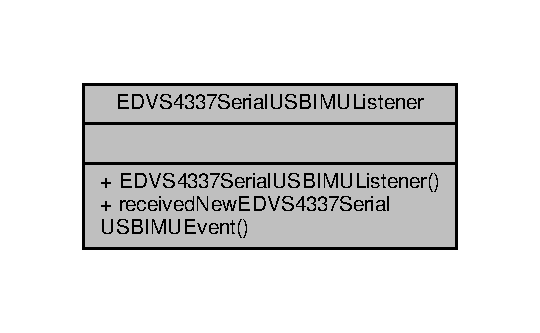
\includegraphics[width=259pt]{class_e_d_v_s4337_serial_u_s_b_i_m_u_listener__coll__graph}
\end{center}
\end{figure}
\subsection*{Public Member Functions}
\begin{DoxyCompactItemize}
\item 
\hypertarget{class_e_d_v_s4337_serial_u_s_b_i_m_u_listener_a6af28f0e3817f55e5dbc3640d9aea378}{}virtual void \hyperlink{class_e_d_v_s4337_serial_u_s_b_i_m_u_listener_a6af28f0e3817f55e5dbc3640d9aea378}{received\+New\+E\+D\+V\+S4337\+Serial\+U\+S\+B\+I\+M\+U\+Event} (\hyperlink{struct_e_d_v_s4337_serial_u_s_b_i_m_u_event}{E\+D\+V\+S4337\+Serial\+U\+S\+B\+I\+M\+U\+Event} \&event)=0\label{class_e_d_v_s4337_serial_u_s_b_i_m_u_listener_a6af28f0e3817f55e5dbc3640d9aea378}

\begin{DoxyCompactList}\small\item\em Is invoked when a new event is parsed from the event stream. \end{DoxyCompactList}\end{DoxyCompactItemize}


\subsection{Detailed Description}
abstract base class for a listener that observers I\+M\+U events 

needs to be subclassed and the reimplement the abstract function received\+New\+E\+D\+V\+S4337\+Serial\+U\+S\+B\+I\+M\+U\+Event 

The documentation for this class was generated from the following file\+:\begin{DoxyCompactItemize}
\item 
/home/serge/\+Documents/\+Semester Project I\+N\+I/omnibot-\/lib/\+U\+S\+B\+\_\+robot/include/\hyperlink{_e_b_v___e_d_v_s4337_serial_u_s_b_8h}{E\+B\+V\+\_\+\+E\+D\+V\+S4337\+Serial\+U\+S\+B.\+h}\end{DoxyCompactItemize}

\hypertarget{class_e_d_v_s4337_serial_u_s_b_listener}{}\section{E\+D\+V\+S4337\+Serial\+U\+S\+B\+Listener Class Reference}
\label{class_e_d_v_s4337_serial_u_s_b_listener}\index{E\+D\+V\+S4337\+Serial\+U\+S\+B\+Listener@{E\+D\+V\+S4337\+Serial\+U\+S\+B\+Listener}}


abstract base class for a listener that observers e\+D\+V\+S events  




{\ttfamily \#include $<$E\+B\+V\+\_\+\+E\+D\+V\+S4337\+Serial\+U\+S\+B.\+h$>$}



Inheritance diagram for E\+D\+V\+S4337\+Serial\+U\+S\+B\+Listener\+:
\nopagebreak
\begin{figure}[H]
\begin{center}
\leavevmode
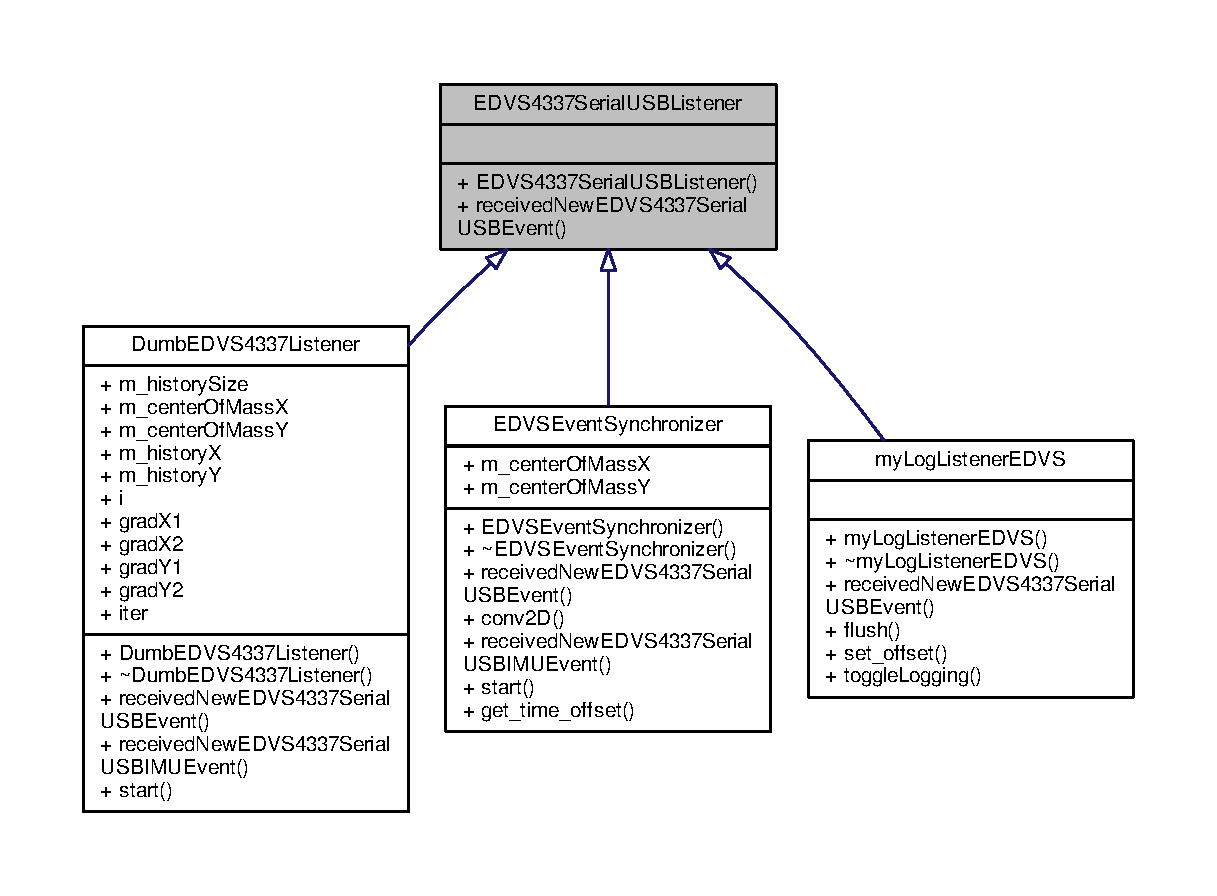
\includegraphics[width=350pt]{class_e_d_v_s4337_serial_u_s_b_listener__inherit__graph}
\end{center}
\end{figure}


Collaboration diagram for E\+D\+V\+S4337\+Serial\+U\+S\+B\+Listener\+:
\nopagebreak
\begin{figure}[H]
\begin{center}
\leavevmode
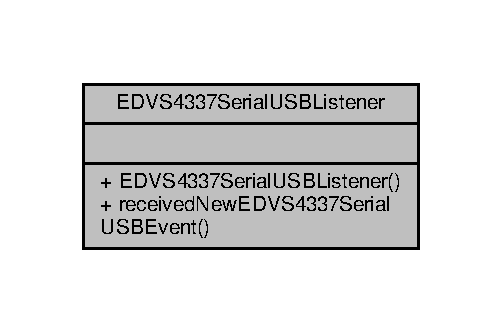
\includegraphics[width=241pt]{class_e_d_v_s4337_serial_u_s_b_listener__coll__graph}
\end{center}
\end{figure}
\subsection*{Public Member Functions}
\begin{DoxyCompactItemize}
\item 
\hypertarget{class_e_d_v_s4337_serial_u_s_b_listener_abb1e87a2ef5c6eaea808b52a73c36e62}{}virtual void \hyperlink{class_e_d_v_s4337_serial_u_s_b_listener_abb1e87a2ef5c6eaea808b52a73c36e62}{received\+New\+E\+D\+V\+S4337\+Serial\+U\+S\+B\+Event} (\hyperlink{struct_e_d_v_s4337_serial_u_s_b_event}{E\+D\+V\+S4337\+Serial\+U\+S\+B\+Event} \&event)=0\label{class_e_d_v_s4337_serial_u_s_b_listener_abb1e87a2ef5c6eaea808b52a73c36e62}

\begin{DoxyCompactList}\small\item\em Is invoked when a new event is parsed from the event stream. \end{DoxyCompactList}\end{DoxyCompactItemize}


\subsection{Detailed Description}
abstract base class for a listener that observers e\+D\+V\+S events 

needs to be subclassed and the reimplement the abstract function received\+New\+E\+D\+V\+S4337\+Serial\+U\+S\+B\+Event 

The documentation for this class was generated from the following file\+:\begin{DoxyCompactItemize}
\item 
/home/serge/\+Documents/\+Semester Project I\+N\+I/omnibot-\/lib/\+U\+S\+B\+\_\+robot/include/\hyperlink{_e_b_v___e_d_v_s4337_serial_u_s_b_8h}{E\+B\+V\+\_\+\+E\+D\+V\+S4337\+Serial\+U\+S\+B.\+h}\end{DoxyCompactItemize}

\hypertarget{class_e_d_v_s_event_synchronizer}{}\section{E\+D\+V\+S\+Event\+Synchronizer Class Reference}
\label{class_e_d_v_s_event_synchronizer}\index{E\+D\+V\+S\+Event\+Synchronizer@{E\+D\+V\+S\+Event\+Synchronizer}}


determines the offset between the timestamps from the E\+D\+V\+S and the computer  




{\ttfamily \#include $<$E\+D\+V\+S\+Event\+Synchronizer.\+h$>$}



Inheritance diagram for E\+D\+V\+S\+Event\+Synchronizer\+:
\nopagebreak
\begin{figure}[H]
\begin{center}
\leavevmode
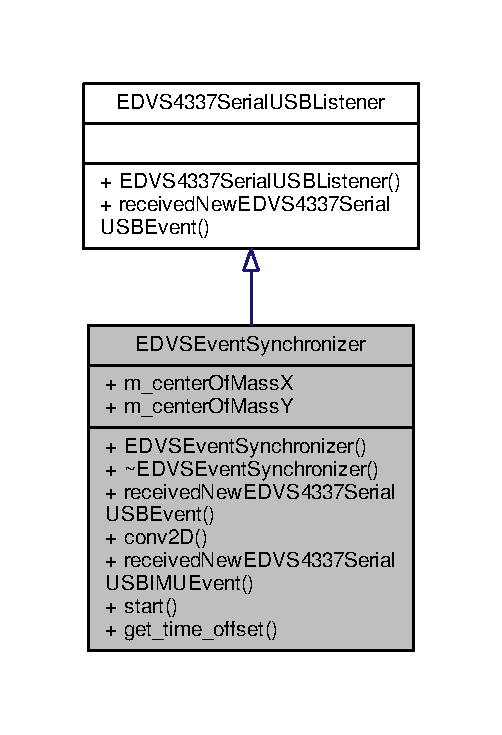
\includegraphics[width=241pt]{class_e_d_v_s_event_synchronizer__inherit__graph}
\end{center}
\end{figure}


Collaboration diagram for E\+D\+V\+S\+Event\+Synchronizer\+:
\nopagebreak
\begin{figure}[H]
\begin{center}
\leavevmode
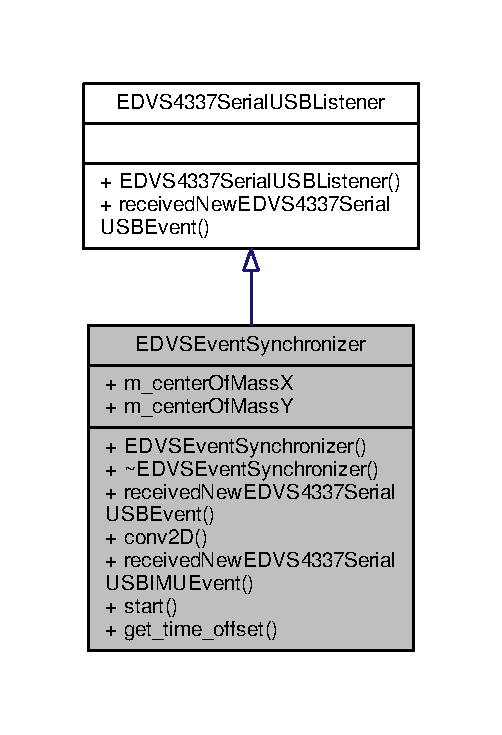
\includegraphics[width=241pt]{class_e_d_v_s_event_synchronizer__coll__graph}
\end{center}
\end{figure}
\subsection*{Public Member Functions}
\begin{DoxyCompactItemize}
\item 
\hyperlink{class_e_d_v_s_event_synchronizer_a3aa2f9f7703a260c2ee77931a41e9a5d}{E\+D\+V\+S\+Event\+Synchronizer} (boost\+::chrono\+::system\+\_\+clock\+::time\+\_\+point orig\+\_\+ts)
\item 
\hypertarget{class_e_d_v_s_event_synchronizer_abf2c8deddd912203f1028d0da0898210}{}void \hyperlink{class_e_d_v_s_event_synchronizer_abf2c8deddd912203f1028d0da0898210}{received\+New\+E\+D\+V\+S4337\+Serial\+U\+S\+B\+Event} (\hyperlink{struct_e_d_v_s4337_serial_u_s_b_event}{E\+D\+V\+S4337\+Serial\+U\+S\+B\+Event} \&e)\label{class_e_d_v_s_event_synchronizer_abf2c8deddd912203f1028d0da0898210}

\begin{DoxyCompactList}\small\item\em Is invoked when a new event is parsed from the event stream. \end{DoxyCompactList}\item 
\hypertarget{class_e_d_v_s_event_synchronizer_ae87bfda7bd247daebf8e59d0044a755b}{}int \hyperlink{class_e_d_v_s_event_synchronizer_ae87bfda7bd247daebf8e59d0044a755b}{conv2\+D} (int x, int y)\label{class_e_d_v_s_event_synchronizer_ae87bfda7bd247daebf8e59d0044a755b}

\begin{DoxyCompactList}\small\item\em converts the 2\+D point indices with respect to the current center of mass to an 1\+D index of an array \end{DoxyCompactList}\item 
\hypertarget{class_e_d_v_s_event_synchronizer_a604261b8dc3e589b6ccde5b89db2dce2}{}void {\bfseries received\+New\+E\+D\+V\+S4337\+Serial\+U\+S\+B\+I\+M\+U\+Event} (\hyperlink{struct_e_d_v_s4337_serial_u_s_b_i_m_u_event}{E\+D\+V\+S4337\+Serial\+U\+S\+B\+I\+M\+U\+Event} \&e)\label{class_e_d_v_s_event_synchronizer_a604261b8dc3e589b6ccde5b89db2dce2}

\item 
\hypertarget{class_e_d_v_s_event_synchronizer_ad6d39f82fd21ab6fee7d1afebd8eb59b}{}void {\bfseries start} (void)\label{class_e_d_v_s_event_synchronizer_ad6d39f82fd21ab6fee7d1afebd8eb59b}

\item 
\hypertarget{class_e_d_v_s_event_synchronizer_a6062d70d3ce2982494fe7dfcaa0f220a}{}double \hyperlink{class_e_d_v_s_event_synchronizer_a6062d70d3ce2982494fe7dfcaa0f220a}{get\+\_\+time\+\_\+offset} ()\label{class_e_d_v_s_event_synchronizer_a6062d70d3ce2982494fe7dfcaa0f220a}

\begin{DoxyCompactList}\small\item\em return the time offset between computer and e\+D\+V\+S in us \end{DoxyCompactList}\end{DoxyCompactItemize}
\subsection*{Public Attributes}
\begin{DoxyCompactItemize}
\item 
\hypertarget{class_e_d_v_s_event_synchronizer_ac5ef909240b8e9dbb3ed30d8554aa23d}{}float {\bfseries m\+\_\+center\+Of\+Mass\+X}\label{class_e_d_v_s_event_synchronizer_ac5ef909240b8e9dbb3ed30d8554aa23d}

\item 
\hypertarget{class_e_d_v_s_event_synchronizer_a6f6cd3e456de1dda22c570f1cbbc9d55}{}float {\bfseries m\+\_\+center\+Of\+Mass\+Y}\label{class_e_d_v_s_event_synchronizer_a6f6cd3e456de1dda22c570f1cbbc9d55}

\end{DoxyCompactItemize}


\subsection{Detailed Description}
determines the offset between the timestamps from the E\+D\+V\+S and the computer 

This is needed as we need to synchronize all events from different sources, like E\+D\+V\+S, keyboard input and information from robots and other devices. To do this calibration a flashing window is displayed on the laptop and the e\+D\+V\+S has to be pointed to it. The calibration is then started by pressing the key \textquotesingle{}o\textquotesingle{}. For debugging purposes the events are displayed in a separate window, as well as the center of mass of the image. 

\subsection{Constructor \& Destructor Documentation}
\hypertarget{class_e_d_v_s_event_synchronizer_a3aa2f9f7703a260c2ee77931a41e9a5d}{}\index{E\+D\+V\+S\+Event\+Synchronizer@{E\+D\+V\+S\+Event\+Synchronizer}!E\+D\+V\+S\+Event\+Synchronizer@{E\+D\+V\+S\+Event\+Synchronizer}}
\index{E\+D\+V\+S\+Event\+Synchronizer@{E\+D\+V\+S\+Event\+Synchronizer}!E\+D\+V\+S\+Event\+Synchronizer@{E\+D\+V\+S\+Event\+Synchronizer}}
\subsubsection[{E\+D\+V\+S\+Event\+Synchronizer}]{\setlength{\rightskip}{0pt plus 5cm}E\+D\+V\+S\+Event\+Synchronizer\+::\+E\+D\+V\+S\+Event\+Synchronizer (
\begin{DoxyParamCaption}
\item[{boost\+::chrono\+::system\+\_\+clock\+::time\+\_\+point}]{orig\+\_\+ts}
\end{DoxyParamCaption}
)}\label{class_e_d_v_s_event_synchronizer_a3aa2f9f7703a260c2ee77931a41e9a5d}

\begin{DoxyParams}{Parameters}
{\em orig\+\_\+ts} & is the timestamp delivered by the computer \\
\hline
\end{DoxyParams}


The documentation for this class was generated from the following files\+:\begin{DoxyCompactItemize}
\item 
/home/serge/\+Documents/\+Semester Project I\+N\+I/omnibot-\/lib/\+U\+S\+B\+\_\+robot/include/E\+D\+V\+S\+Event\+Synchronizer.\+h\item 
/home/serge/\+Documents/\+Semester Project I\+N\+I/omnibot-\/lib/\+U\+S\+B\+\_\+robot/src/E\+D\+V\+S\+Event\+Synchronizer.\+cpp\end{DoxyCompactItemize}

\hypertarget{structkeyboard__state}{}\section{keyboard\+\_\+state Struct Reference}
\label{structkeyboard__state}\index{keyboard\+\_\+state@{keyboard\+\_\+state}}


encapsulates the states of all the avaiable keyboard keys  




{\ttfamily \#include $<$keyboard.\+h$>$}



Collaboration diagram for keyboard\+\_\+state\+:
\nopagebreak
\begin{figure}[H]
\begin{center}
\leavevmode
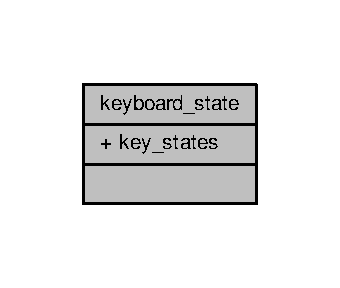
\includegraphics[width=163pt]{structkeyboard__state__coll__graph}
\end{center}
\end{figure}
\subsection*{Public Attributes}
\begin{DoxyCompactItemize}
\item 
\hypertarget{structkeyboard__state_a185511b91db240cbfe49dbe92d5e88cb}{}unsigned short \hyperlink{structkeyboard__state_a185511b91db240cbfe49dbe92d5e88cb}{key\+\_\+states} \mbox{[}K\+E\+Y\+\_\+\+C\+N\+T\mbox{]}\label{structkeyboard__state_a185511b91db240cbfe49dbe92d5e88cb}

\begin{DoxyCompactList}\small\item\em array with all the avaiable keyboard keys. 0 means the key is released, 1 pressed and 2 that it is repeated ( = held down) \end{DoxyCompactList}\end{DoxyCompactItemize}


\subsection{Detailed Description}
encapsulates the states of all the avaiable keyboard keys 

The documentation for this struct was generated from the following file\+:\begin{DoxyCompactItemize}
\item 
/home/serge/\+Documents/\+Semester Project I\+N\+I/omnibot-\/lib/\+U\+S\+B\+\_\+robot/include/\hyperlink{keyboard_8h}{keyboard.\+h}\end{DoxyCompactItemize}

\hypertarget{class_keyboard_listener}{}\section{Keyboard\+Listener Class Reference}
\label{class_keyboard_listener}\index{Keyboard\+Listener@{Keyboard\+Listener}}


Provides the necessary interface to Listen to keyboard events.  




{\ttfamily \#include $<$keyboard.\+h$>$}



Inheritance diagram for Keyboard\+Listener\+:
\nopagebreak
\begin{figure}[H]
\begin{center}
\leavevmode
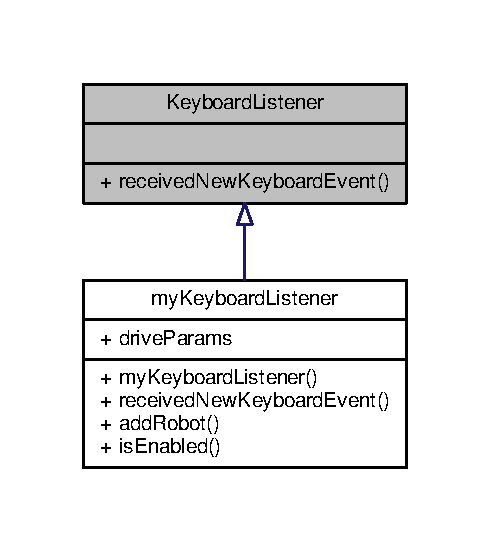
\includegraphics[width=235pt]{class_keyboard_listener__inherit__graph}
\end{center}
\end{figure}


Collaboration diagram for Keyboard\+Listener\+:
\nopagebreak
\begin{figure}[H]
\begin{center}
\leavevmode
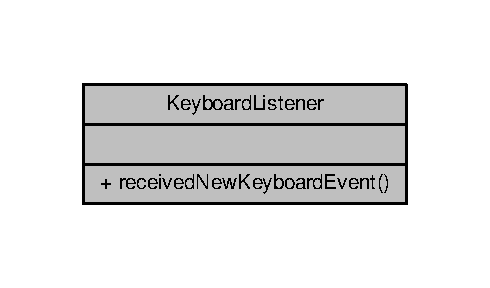
\includegraphics[width=235pt]{class_keyboard_listener__coll__graph}
\end{center}
\end{figure}
\subsection*{Public Member Functions}
\begin{DoxyCompactItemize}
\item 
\hypertarget{class_keyboard_listener_ac9751e8976e26e8733ee6086b313c93d}{}virtual void \hyperlink{class_keyboard_listener_ac9751e8976e26e8733ee6086b313c93d}{received\+New\+Keyboard\+Event} (input\+\_\+event $\ast$)=0\label{class_keyboard_listener_ac9751e8976e26e8733ee6086b313c93d}

\begin{DoxyCompactList}\small\item\em is emitted from a \hyperlink{classc_keyboard}{c\+Keyboard} object when a new keystroke has been registered. \end{DoxyCompactList}\end{DoxyCompactItemize}


\subsection{Detailed Description}
Provides the necessary interface to Listen to keyboard events. 

The documentation for this class was generated from the following file\+:\begin{DoxyCompactItemize}
\item 
/home/serge/\+Documents/\+Semester Project I\+N\+I/omnibot-\/lib/\+U\+S\+B\+\_\+robot/include/\hyperlink{keyboard_8h}{keyboard.\+h}\end{DoxyCompactItemize}

\hypertarget{classmy_keyboard_listener}{}\section{my\+Keyboard\+Listener Class Reference}
\label{classmy_keyboard_listener}\index{my\+Keyboard\+Listener@{my\+Keyboard\+Listener}}


Inheritance diagram for my\+Keyboard\+Listener\+:
\nopagebreak
\begin{figure}[H]
\begin{center}
\leavevmode
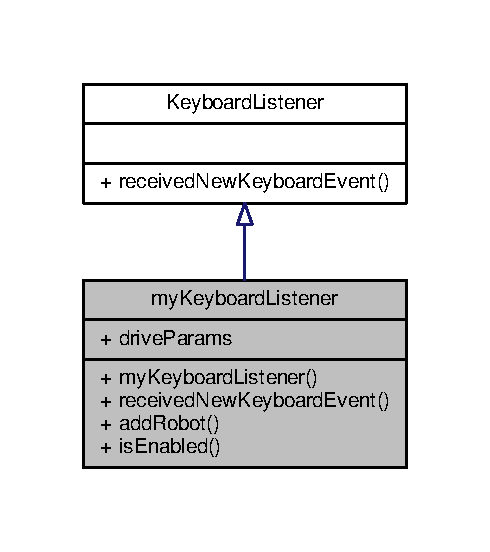
\includegraphics[width=235pt]{classmy_keyboard_listener__inherit__graph}
\end{center}
\end{figure}


Collaboration diagram for my\+Keyboard\+Listener\+:
\nopagebreak
\begin{figure}[H]
\begin{center}
\leavevmode
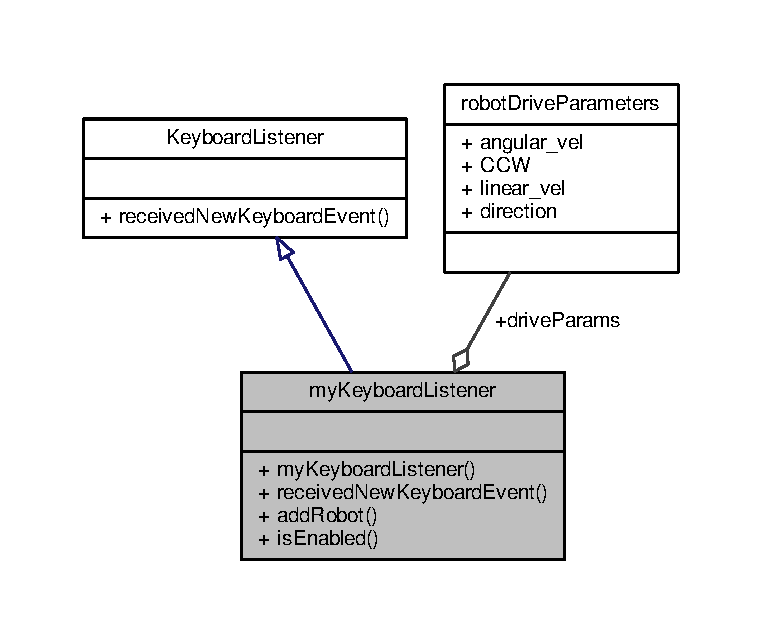
\includegraphics[width=350pt]{classmy_keyboard_listener__coll__graph}
\end{center}
\end{figure}
\subsection*{Public Member Functions}
\begin{DoxyCompactItemize}
\item 
\hypertarget{classmy_keyboard_listener_a38e4fe0293a178aa108a092928c69f13}{}void \hyperlink{classmy_keyboard_listener_a38e4fe0293a178aa108a092928c69f13}{received\+New\+Keyboard\+Event} (input\+\_\+event $\ast$)\label{classmy_keyboard_listener_a38e4fe0293a178aa108a092928c69f13}

\begin{DoxyCompactList}\small\item\em is emitted from a \hyperlink{classc_keyboard}{c\+Keyboard} object when a new keystroke has been registered. \end{DoxyCompactList}\item 
\hypertarget{classmy_keyboard_listener_a58bbdff3ddabad3be69842425bd7137e}{}void {\bfseries add\+Robot} (\hyperlink{class_robot}{Robot} $\ast$)\label{classmy_keyboard_listener_a58bbdff3ddabad3be69842425bd7137e}

\item 
\hypertarget{classmy_keyboard_listener_ab872b8eea1b5b74f24bb67d456e8ce1d}{}bool {\bfseries is\+Enabled} ()\label{classmy_keyboard_listener_ab872b8eea1b5b74f24bb67d456e8ce1d}

\end{DoxyCompactItemize}
\subsection*{Public Attributes}
\begin{DoxyCompactItemize}
\item 
\hypertarget{classmy_keyboard_listener_ac5e0ea7bc8dbff0501aaac437fcc17b9}{}\hyperlink{structrobot_drive_parameters}{robot\+Drive\+Parameters} $\ast$ {\bfseries drive\+Params}\label{classmy_keyboard_listener_ac5e0ea7bc8dbff0501aaac437fcc17b9}

\end{DoxyCompactItemize}


The documentation for this class was generated from the following files\+:\begin{DoxyCompactItemize}
\item 
/home/serge/\+Documents/\+Semester Project I\+N\+I/omnibot-\/lib/\+U\+S\+B\+\_\+robot/include/\hyperlink{my_keyboard_listener_8h}{my\+Keyboard\+Listener.\+h}\item 
/home/serge/\+Documents/\+Semester Project I\+N\+I/omnibot-\/lib/\+U\+S\+B\+\_\+robot/src/my\+Keyboard\+Listener.\+cpp\end{DoxyCompactItemize}

\hypertarget{classmy_log_listener_e_d_v_s}{}\section{my\+Log\+Listener\+E\+D\+V\+S Class Reference}
\label{classmy_log_listener_e_d_v_s}\index{my\+Log\+Listener\+E\+D\+V\+S@{my\+Log\+Listener\+E\+D\+V\+S}}


This class provides a concrete implementation of a e\+D\+V\+S event listener that logs the received events to a file.  




{\ttfamily \#include $<$my\+Log\+Listener\+E\+D\+V\+S.\+h$>$}



Inheritance diagram for my\+Log\+Listener\+E\+D\+V\+S\+:
\nopagebreak
\begin{figure}[H]
\begin{center}
\leavevmode
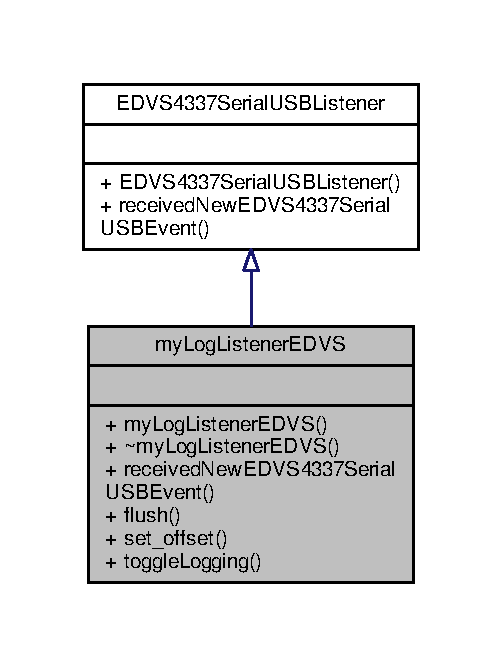
\includegraphics[width=241pt]{classmy_log_listener_e_d_v_s__inherit__graph}
\end{center}
\end{figure}


Collaboration diagram for my\+Log\+Listener\+E\+D\+V\+S\+:
\nopagebreak
\begin{figure}[H]
\begin{center}
\leavevmode
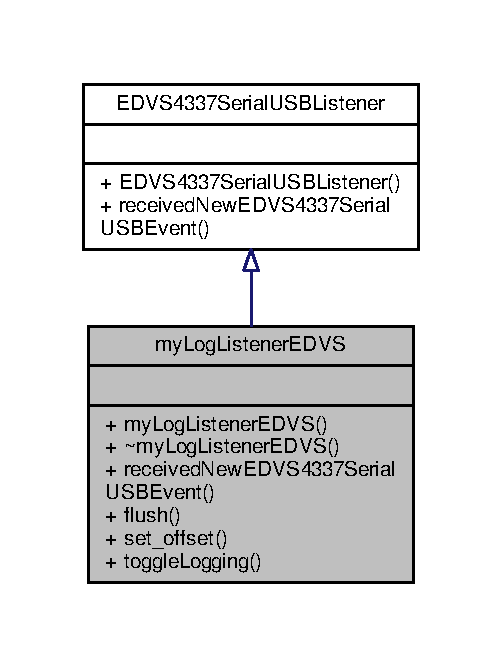
\includegraphics[width=241pt]{classmy_log_listener_e_d_v_s__coll__graph}
\end{center}
\end{figure}
\subsection*{Public Member Functions}
\begin{DoxyCompactItemize}
\item 
\hypertarget{classmy_log_listener_e_d_v_s_acf61bf49fd9cf235a4498411b44e9aa2}{}\hyperlink{classmy_log_listener_e_d_v_s_acf61bf49fd9cf235a4498411b44e9aa2}{my\+Log\+Listener\+E\+D\+V\+S} ()\label{classmy_log_listener_e_d_v_s_acf61bf49fd9cf235a4498411b44e9aa2}

\begin{DoxyCompactList}\small\item\em constructor, takeas also care of opening a log file. \end{DoxyCompactList}\item 
\hypertarget{classmy_log_listener_e_d_v_s_ac2c38d50f2e0830ac3f4433608939997}{}\hyperlink{classmy_log_listener_e_d_v_s_ac2c38d50f2e0830ac3f4433608939997}{$\sim$my\+Log\+Listener\+E\+D\+V\+S} ()\label{classmy_log_listener_e_d_v_s_ac2c38d50f2e0830ac3f4433608939997}

\begin{DoxyCompactList}\small\item\em destructor, flushes the reamining events to the file and closes the file. \end{DoxyCompactList}\item 
\hypertarget{classmy_log_listener_e_d_v_s_a1777d000440b6f85d49dd49ff89b2429}{}void \hyperlink{classmy_log_listener_e_d_v_s_a1777d000440b6f85d49dd49ff89b2429}{received\+New\+E\+D\+V\+S4337\+Serial\+U\+S\+B\+Event} (\hyperlink{struct_e_d_v_s4337_serial_u_s_b_event}{E\+D\+V\+S4337\+Serial\+U\+S\+B\+Event} \&e)\label{classmy_log_listener_e_d_v_s_a1777d000440b6f85d49dd49ff89b2429}

\begin{DoxyCompactList}\small\item\em events come one by one, \end{DoxyCompactList}\item 
\hypertarget{classmy_log_listener_e_d_v_s_a765267309b967a51266bec88b618dae4}{}void \hyperlink{classmy_log_listener_e_d_v_s_a765267309b967a51266bec88b618dae4}{flush} ()\label{classmy_log_listener_e_d_v_s_a765267309b967a51266bec88b618dae4}

\begin{DoxyCompactList}\small\item\em writes all remaining events to the log file \end{DoxyCompactList}\item 
\hypertarget{classmy_log_listener_e_d_v_s_a98d36489262e95d277ba8183443d2b85}{}void \hyperlink{classmy_log_listener_e_d_v_s_a98d36489262e95d277ba8183443d2b85}{set\+\_\+offset} (double dt)\label{classmy_log_listener_e_d_v_s_a98d36489262e95d277ba8183443d2b85}

\begin{DoxyCompactList}\small\item\em e\+D\+V\+S has an ofset with respect to the clock of the host computer and therefore the keyboard and robot events \end{DoxyCompactList}\item 
\hypertarget{classmy_log_listener_e_d_v_s_aca2a9088907f9b0ab265aa4d3cd32ba4}{}void \hyperlink{classmy_log_listener_e_d_v_s_aca2a9088907f9b0ab265aa4d3cd32ba4}{toggle\+Logging} ()\label{classmy_log_listener_e_d_v_s_aca2a9088907f9b0ab265aa4d3cd32ba4}

\begin{DoxyCompactList}\small\item\em toggle logging \end{DoxyCompactList}\end{DoxyCompactItemize}


\subsection{Detailed Description}
This class provides a concrete implementation of a e\+D\+V\+S event listener that logs the received events to a file. 

The documentation for this class was generated from the following files\+:\begin{DoxyCompactItemize}
\item 
/home/serge/\+Documents/\+Semester Project I\+N\+I/omnibot-\/lib/\+U\+S\+B\+\_\+robot/include/\hyperlink{my_log_listener_e_d_v_s_8h}{my\+Log\+Listener\+E\+D\+V\+S.\+h}\item 
/home/serge/\+Documents/\+Semester Project I\+N\+I/omnibot-\/lib/\+U\+S\+B\+\_\+robot/src/my\+Log\+Listener\+E\+D\+V\+S.\+cpp\end{DoxyCompactItemize}

\hypertarget{classmy_log_listener_robot}{}\section{my\+Log\+Listener\+Robot Class Reference}
\label{classmy_log_listener_robot}\index{my\+Log\+Listener\+Robot@{my\+Log\+Listener\+Robot}}


Provides a concrete implementation of the abstract \hyperlink{class_robot_listener}{Robot\+Listener} to receive the servo states and the bumber states parsed from the robot event stream.  




{\ttfamily \#include $<$my\+Log\+Listener\+Robot.\+h$>$}



Inheritance diagram for my\+Log\+Listener\+Robot\+:
\nopagebreak
\begin{figure}[H]
\begin{center}
\leavevmode
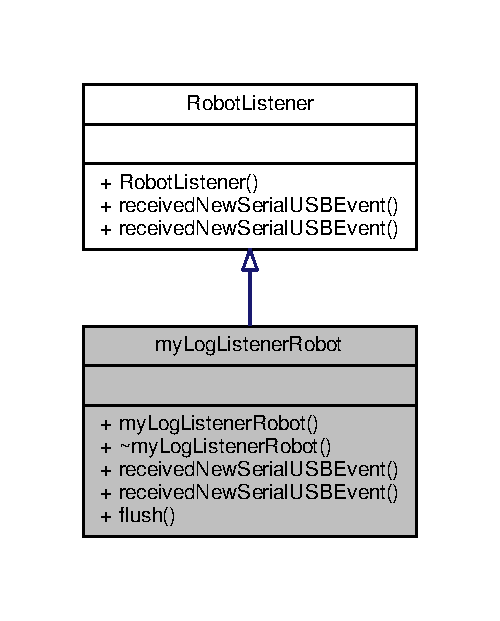
\includegraphics[width=240pt]{classmy_log_listener_robot__inherit__graph}
\end{center}
\end{figure}


Collaboration diagram for my\+Log\+Listener\+Robot\+:
\nopagebreak
\begin{figure}[H]
\begin{center}
\leavevmode
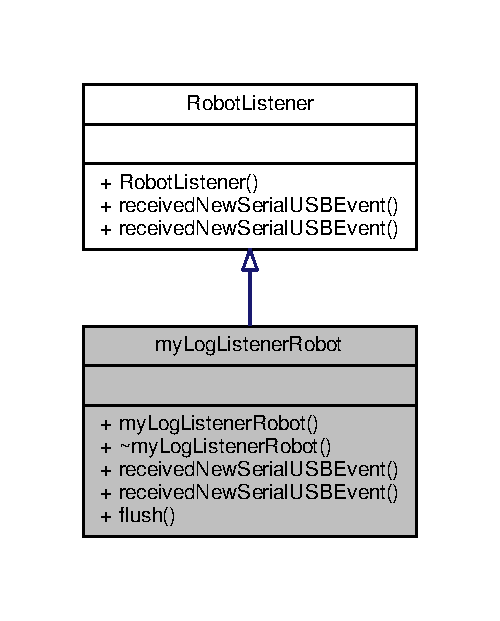
\includegraphics[width=240pt]{classmy_log_listener_robot__coll__graph}
\end{center}
\end{figure}
\subsection*{Public Member Functions}
\begin{DoxyCompactItemize}
\item 
\hypertarget{classmy_log_listener_robot_a19d65e6a5c0e14c9e08e8d1ffb23a709}{}void \hyperlink{classmy_log_listener_robot_a19d65e6a5c0e14c9e08e8d1ffb23a709}{received\+New\+Serial\+U\+S\+B\+Event} (std\+::queue$<$ \hyperlink{structservo_signals}{servo\+Signals} $>$ \&)\label{classmy_log_listener_robot_a19d65e6a5c0e14c9e08e8d1ffb23a709}

\begin{DoxyCompactList}\small\item\em receives the decoded servos states from the observed robot \end{DoxyCompactList}\item 
\hypertarget{classmy_log_listener_robot_a2fbd30aaa4a439e3d4e4b4ac812596c9}{}void \hyperlink{classmy_log_listener_robot_a2fbd30aaa4a439e3d4e4b4ac812596c9}{received\+New\+Serial\+U\+S\+B\+Event} (std\+::queue$<$ \hyperlink{structbumper}{bumper} $>$ \&)\label{classmy_log_listener_robot_a2fbd30aaa4a439e3d4e4b4ac812596c9}

\begin{DoxyCompactList}\small\item\em receives the decoded bumber events from the observed robot \end{DoxyCompactList}\item 
\hypertarget{classmy_log_listener_robot_a0e9b99ec81b173cad06d161c86cb86d8}{}void {\bfseries flush} ()\label{classmy_log_listener_robot_a0e9b99ec81b173cad06d161c86cb86d8}

\end{DoxyCompactItemize}


\subsection{Detailed Description}
Provides a concrete implementation of the abstract \hyperlink{class_robot_listener}{Robot\+Listener} to receive the servo states and the bumber states parsed from the robot event stream. 

The documentation for this class was generated from the following files\+:\begin{DoxyCompactItemize}
\item 
/home/serge/\+Documents/\+Semester Project I\+N\+I/omnibot-\/lib/\+U\+S\+B\+\_\+robot/include/my\+Log\+Listener\+Robot.\+h\item 
/home/serge/\+Documents/\+Semester Project I\+N\+I/omnibot-\/lib/\+U\+S\+B\+\_\+robot/src/my\+Log\+Listener\+Robot.\+cpp\end{DoxyCompactItemize}

\hypertarget{class_omni_robot}{}\section{Omni\+Robot Class Reference}
\label{class_omni_robot}\index{Omni\+Robot@{Omni\+Robot}}


Interface to the Omni\+Rob from N\+S\+T.  




{\ttfamily \#include $<$Omni\+Robot.\+h$>$}



Inheritance diagram for Omni\+Robot\+:
\nopagebreak
\begin{figure}[H]
\begin{center}
\leavevmode
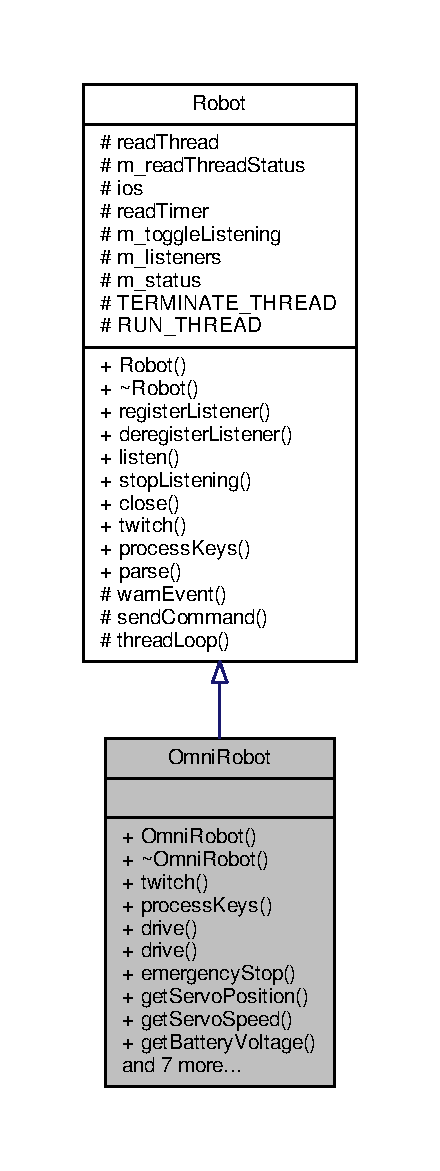
\includegraphics[height=550pt]{class_omni_robot__inherit__graph}
\end{center}
\end{figure}


Collaboration diagram for Omni\+Robot\+:
\nopagebreak
\begin{figure}[H]
\begin{center}
\leavevmode
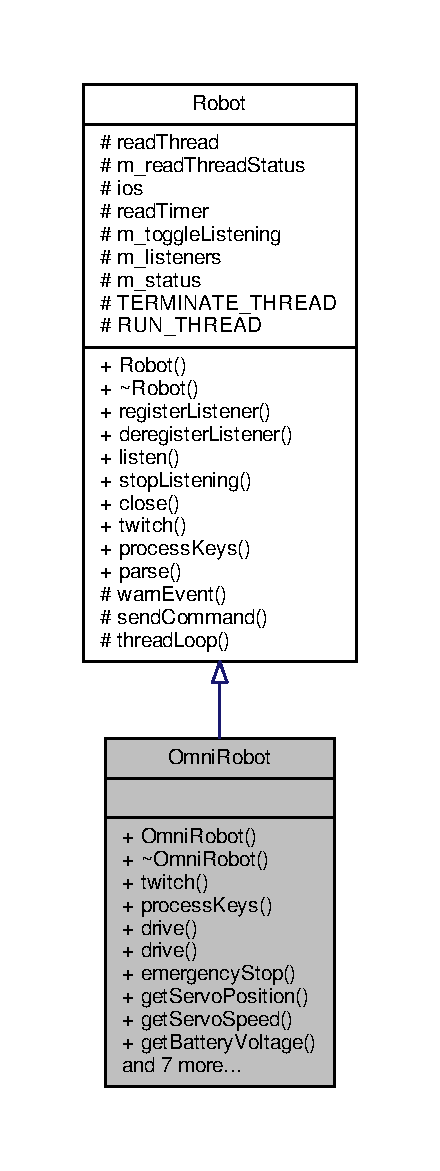
\includegraphics[height=550pt]{class_omni_robot__coll__graph}
\end{center}
\end{figure}
\subsection*{Public Member Functions}
\begin{DoxyCompactItemize}
\item 
\hyperlink{class_omni_robot_a0adede977dc636bdc42c99edb148d176}{Omni\+Robot} (int file\+Descriptor)
\begin{DoxyCompactList}\small\item\em Constructor. \end{DoxyCompactList}\item 
\hypertarget{class_omni_robot_aa1fdc3c89c1cc303fc2416142af847ba}{}bool \hyperlink{class_omni_robot_aa1fdc3c89c1cc303fc2416142af847ba}{twitch} ()\label{class_omni_robot_aa1fdc3c89c1cc303fc2416142af847ba}

\begin{DoxyCompactList}\small\item\em test Omni\+Rob when first connecting \end{DoxyCompactList}\item 
\hypertarget{class_omni_robot_a9098e781569c5da8c5fdd16be6310866}{}void \hyperlink{class_omni_robot_a9098e781569c5da8c5fdd16be6310866}{process\+Keys} (int keys\+Pressed)\label{class_omni_robot_a9098e781569c5da8c5fdd16be6310866}

\begin{DoxyCompactList}\small\item\em process the keys logged from the keyboard \end{DoxyCompactList}\item 
void \hyperlink{class_omni_robot_a4bf623e941d12271de06a3feca707f1f}{drive} (double angular\+\_\+vel, bool C\+C\+W, double linear\+\_\+vel, double direction)
\begin{DoxyCompactList}\small\item\em Make the robot move. \end{DoxyCompactList}\item 
void \hyperlink{class_omni_robot_ad0719d67222bcea330964a193d8bf717}{drive} ()
\begin{DoxyCompactList}\small\item\em drive the robot after setting the drive parameters. \end{DoxyCompactList}\item 
\hypertarget{class_omni_robot_af8a7e63e307d39cd63f9ad8ff1b8f438}{}void \hyperlink{class_omni_robot_af8a7e63e307d39cd63f9ad8ff1b8f438}{emergency\+Stop} ()\label{class_omni_robot_af8a7e63e307d39cd63f9ad8ff1b8f438}

\begin{DoxyCompactList}\small\item\em stop the robot immediatly and set its drive states to 0 \end{DoxyCompactList}\item 
void \hyperlink{class_omni_robot_a4990bacab4be83a14508ef4a6859a2a5}{get\+Servo\+Position} (int servo\+I\+D, int $\ast$signal)
\begin{DoxyCompactList}\small\item\em get the last logged position of servo i \end{DoxyCompactList}\item 
void \hyperlink{class_omni_robot_af6051abc3663618772fcf690445cac14}{get\+Servo\+Speed} (int servo\+I\+D, int $\ast$signal)
\begin{DoxyCompactList}\small\item\em get the last logged speed of servo in terms of servo signal \end{DoxyCompactList}\item 
\hypertarget{class_omni_robot_a41817e196ad64ba61daa8bbcc4ccc6c2}{}int \hyperlink{class_omni_robot_a41817e196ad64ba61daa8bbcc4ccc6c2}{get\+Battery\+Voltage} ()\label{class_omni_robot_a41817e196ad64ba61daa8bbcc4ccc6c2}

\begin{DoxyCompactList}\small\item\em get the last logged battery voltage \end{DoxyCompactList}\item 
void \hyperlink{class_omni_robot_a5ccec8006487e526b20e7a5f69255c00}{set\+Robot\+Drive\+State} (const \hyperlink{structrobot_drive_state}{robot\+Drive\+State} \&)
\begin{DoxyCompactList}\small\item\em set the robot drive state, but do not drive yet \end{DoxyCompactList}\item 
\hypertarget{class_omni_robot_a4db727ee61666148106e302e90956bd3}{}void \hyperlink{class_omni_robot_a4db727ee61666148106e302e90956bd3}{set\+Servo\+Speed} (int servo\+I\+D, int signal)\label{class_omni_robot_a4db727ee61666148106e302e90956bd3}

\begin{DoxyCompactList}\small\item\em set the speed signal of servo i. Change is applied directly. \end{DoxyCompactList}\item 
void \hyperlink{class_omni_robot_a2f3365750b17b172ef265fb94e25c73a}{set\+Servo\+Speeds} (double $\ast$)
\begin{DoxyCompactList}\small\item\em set the speed signal of all servos. Change is applied directly. \end{DoxyCompactList}\item 
void \hyperlink{class_omni_robot_a01e9c0201e9bcd1ff6b3f3039e910937}{set\+Servo\+Torque} (int servo\+I\+D, bool enable, int signal)
\item 
void \hyperlink{class_omni_robot_a27f0a605b283a8e1a49b5829c656edd8}{parse} (unsigned char $\ast$data, int bytes\+Read)
\begin{DoxyCompactList}\small\item\em parse commands from the sring received from the serial connection \end{DoxyCompactList}\item 
void \hyperlink{class_omni_robot_ad7b2e7cf5cca375cfc9ba047264dfcad}{start\+Logging} ()
\begin{DoxyCompactList}\small\item\em start recording to file \end{DoxyCompactList}\item 
\hypertarget{class_omni_robot_a899ff538efad531b391e84182a6ed961}{}void \hyperlink{class_omni_robot_a899ff538efad531b391e84182a6ed961}{set\+\_\+time\+\_\+origin} (boost\+::chrono\+::system\+\_\+clock\+::time\+\_\+point start)\label{class_omni_robot_a899ff538efad531b391e84182a6ed961}

\begin{DoxyCompactList}\small\item\em set the original timestamp to synchronize with e\+D\+V\+S \end{DoxyCompactList}\end{DoxyCompactItemize}
\subsection*{Additional Inherited Members}


\subsection{Detailed Description}
Interface to the Omni\+Rob from N\+S\+T. 

\subsection{Constructor \& Destructor Documentation}
\hypertarget{class_omni_robot_a0adede977dc636bdc42c99edb148d176}{}\index{Omni\+Robot@{Omni\+Robot}!Omni\+Robot@{Omni\+Robot}}
\index{Omni\+Robot@{Omni\+Robot}!Omni\+Robot@{Omni\+Robot}}
\subsubsection[{Omni\+Robot}]{\setlength{\rightskip}{0pt plus 5cm}Omni\+Robot\+::\+Omni\+Robot (
\begin{DoxyParamCaption}
\item[{int}]{file\+Descriptor}
\end{DoxyParamCaption}
)}\label{class_omni_robot_a0adede977dc636bdc42c99edb148d176}


Constructor. 


\begin{DoxyParams}{Parameters}
{\em file\+Descriptor} & is a valid file descriptor to communication interface with the robot \\
\hline
\end{DoxyParams}
\begin{DoxySeeAlso}{See also}
??? 
\end{DoxySeeAlso}


\subsection{Member Function Documentation}
\hypertarget{class_omni_robot_a4bf623e941d12271de06a3feca707f1f}{}\index{Omni\+Robot@{Omni\+Robot}!drive@{drive}}
\index{drive@{drive}!Omni\+Robot@{Omni\+Robot}}
\subsubsection[{drive}]{\setlength{\rightskip}{0pt plus 5cm}void Omni\+Robot\+::drive (
\begin{DoxyParamCaption}
\item[{double}]{angular\+\_\+vel, }
\item[{bool}]{C\+C\+W, }
\item[{double}]{linear\+\_\+vel, }
\item[{double}]{direction}
\end{DoxyParamCaption}
)}\label{class_omni_robot_a4bf623e941d12271de06a3feca707f1f}


Make the robot move. 

The drive function sets the servo speeds of the robot according to the specified input. 
\begin{DoxyParams}{Parameters}
{\em angular\+\_\+vel} & can take values from 0 to 100, indicating the speed of the servo (0 = off, 100 = maximum). Determines the turning rate of the robot. \\
\hline
{\em C\+C\+W} & determines if the servo is turning C\+C\+W or C\+W \\
\hline
{\em linear\+\_\+vel} & can take values from 0 to 100, indicating the speed of the servo (0 = off, 100 = maximum). Determines the linear velocity of the robot. \\
\hline
{\em direction} & in degrees. Sets the direction where the robot is headed. N\+B\+: The driving vector is in polar coordinates. \\
\hline
\end{DoxyParams}
\hypertarget{class_omni_robot_ad0719d67222bcea330964a193d8bf717}{}\index{Omni\+Robot@{Omni\+Robot}!drive@{drive}}
\index{drive@{drive}!Omni\+Robot@{Omni\+Robot}}
\subsubsection[{drive}]{\setlength{\rightskip}{0pt plus 5cm}void Omni\+Robot\+::drive (
\begin{DoxyParamCaption}
{}
\end{DoxyParamCaption}
)}\label{class_omni_robot_ad0719d67222bcea330964a193d8bf717}


drive the robot after setting the drive parameters. 

\begin{DoxySeeAlso}{See also}
\hyperlink{class_omni_robot_a5ccec8006487e526b20e7a5f69255c00}{set\+Robot\+Drive\+State} 
\end{DoxySeeAlso}
\hypertarget{class_omni_robot_a4990bacab4be83a14508ef4a6859a2a5}{}\index{Omni\+Robot@{Omni\+Robot}!get\+Servo\+Position@{get\+Servo\+Position}}
\index{get\+Servo\+Position@{get\+Servo\+Position}!Omni\+Robot@{Omni\+Robot}}
\subsubsection[{get\+Servo\+Position}]{\setlength{\rightskip}{0pt plus 5cm}void Omni\+Robot\+::get\+Servo\+Position (
\begin{DoxyParamCaption}
\item[{int}]{servo\+I\+D, }
\item[{int $\ast$}]{signal}
\end{DoxyParamCaption}
)}\label{class_omni_robot_a4990bacab4be83a14508ef4a6859a2a5}


get the last logged position of servo i 


\begin{DoxyParams}{Parameters}
{\em servo\+I\+D} & I\+D of the servo \\
\hline
{\em signal} & variable to store the signal value \\
\hline
\end{DoxyParams}
\hypertarget{class_omni_robot_af6051abc3663618772fcf690445cac14}{}\index{Omni\+Robot@{Omni\+Robot}!get\+Servo\+Speed@{get\+Servo\+Speed}}
\index{get\+Servo\+Speed@{get\+Servo\+Speed}!Omni\+Robot@{Omni\+Robot}}
\subsubsection[{get\+Servo\+Speed}]{\setlength{\rightskip}{0pt plus 5cm}void Omni\+Robot\+::get\+Servo\+Speed (
\begin{DoxyParamCaption}
\item[{int}]{servo\+I\+D, }
\item[{int $\ast$}]{signal}
\end{DoxyParamCaption}
)}\label{class_omni_robot_af6051abc3663618772fcf690445cac14}


get the last logged speed of servo in terms of servo signal 


\begin{DoxyParams}{Parameters}
{\em servo\+I\+D} & I\+D of the servo \\
\hline
{\em signal} & variable to store the signal value \\
\hline
\end{DoxyParams}
\hypertarget{class_omni_robot_a27f0a605b283a8e1a49b5829c656edd8}{}\index{Omni\+Robot@{Omni\+Robot}!parse@{parse}}
\index{parse@{parse}!Omni\+Robot@{Omni\+Robot}}
\subsubsection[{parse}]{\setlength{\rightskip}{0pt plus 5cm}void Omni\+Robot\+::parse (
\begin{DoxyParamCaption}
\item[{unsigned char $\ast$}]{data, }
\item[{int}]{bytes\+Read}
\end{DoxyParamCaption}
)\hspace{0.3cm}{\ttfamily [virtual]}}\label{class_omni_robot_a27f0a605b283a8e1a49b5829c656edd8}


parse commands from the sring received from the serial connection 


\begin{DoxyParams}{Parameters}
{\em data} & the data string read from the serial Port \\
\hline
{\em bytes\+Read} & the number of bytes read = length of data \\
\hline
\end{DoxyParams}


Implements \hyperlink{class_robot_a7dcc9de1f4a64894bdc047efd5db8a2b}{Robot}.

\hypertarget{class_omni_robot_a5ccec8006487e526b20e7a5f69255c00}{}\index{Omni\+Robot@{Omni\+Robot}!set\+Robot\+Drive\+State@{set\+Robot\+Drive\+State}}
\index{set\+Robot\+Drive\+State@{set\+Robot\+Drive\+State}!Omni\+Robot@{Omni\+Robot}}
\subsubsection[{set\+Robot\+Drive\+State}]{\setlength{\rightskip}{0pt plus 5cm}void Omni\+Robot\+::set\+Robot\+Drive\+State (
\begin{DoxyParamCaption}
\item[{const {\bf robot\+Drive\+State} \&}]{in\+State}
\end{DoxyParamCaption}
)}\label{class_omni_robot_a5ccec8006487e526b20e7a5f69255c00}


set the robot drive state, but do not drive yet 


\begin{DoxyParams}{Parameters}
{\em \hyperlink{structrobot_drive_state}{robot\+Drive\+State}} & is of type \hyperlink{structrobot_drive_state}{robot\+Drive\+State} and encaplsulates the mid-\/level drive states. \\
\hline
\end{DoxyParams}
\begin{DoxySeeAlso}{See also}
\hyperlink{structrobot_drive_state}{robot\+Drive\+State} 
\end{DoxySeeAlso}
\hypertarget{class_omni_robot_a2f3365750b17b172ef265fb94e25c73a}{}\index{Omni\+Robot@{Omni\+Robot}!set\+Servo\+Speeds@{set\+Servo\+Speeds}}
\index{set\+Servo\+Speeds@{set\+Servo\+Speeds}!Omni\+Robot@{Omni\+Robot}}
\subsubsection[{set\+Servo\+Speeds}]{\setlength{\rightskip}{0pt plus 5cm}void Omni\+Robot\+::set\+Servo\+Speeds (
\begin{DoxyParamCaption}
\item[{double $\ast$}]{signals}
\end{DoxyParamCaption}
)}\label{class_omni_robot_a2f3365750b17b172ef265fb94e25c73a}


set the speed signal of all servos. Change is applied directly. 

It is better to use this function when setting all servos, as the commands are send in one string, which is more effective and mor secure, especially when communicating via Wi\+Fi 
\begin{DoxyParams}{Parameters}
{\em servo\+Speeds\+Array} & array with the servo speeds from lowest to highest servo I\+D. \\
\hline
\end{DoxyParams}
\hypertarget{class_omni_robot_a01e9c0201e9bcd1ff6b3f3039e910937}{}\index{Omni\+Robot@{Omni\+Robot}!set\+Servo\+Torque@{set\+Servo\+Torque}}
\index{set\+Servo\+Torque@{set\+Servo\+Torque}!Omni\+Robot@{Omni\+Robot}}
\subsubsection[{set\+Servo\+Torque}]{\setlength{\rightskip}{0pt plus 5cm}void Omni\+Robot\+::set\+Servo\+Torque (
\begin{DoxyParamCaption}
\item[{int}]{servo\+I\+D, }
\item[{bool}]{enable, }
\item[{int}]{signal}
\end{DoxyParamCaption}
)}\label{class_omni_robot_a01e9c0201e9bcd1ff6b3f3039e910937}
set the torque of servo i. get the last logged speed of servo in terms of servo signal


\begin{DoxyParams}{Parameters}
{\em servo\+I\+D} & I\+D of the servo \\
\hline
{\em enable} & enable or disable servo \\
\hline
{\em signal} & variable to store the signal value \\
\hline
\end{DoxyParams}
\hypertarget{class_omni_robot_ad7b2e7cf5cca375cfc9ba047264dfcad}{}\index{Omni\+Robot@{Omni\+Robot}!start\+Logging@{start\+Logging}}
\index{start\+Logging@{start\+Logging}!Omni\+Robot@{Omni\+Robot}}
\subsubsection[{start\+Logging}]{\setlength{\rightskip}{0pt plus 5cm}void Omni\+Robot\+::start\+Logging (
\begin{DoxyParamCaption}
{}
\end{DoxyParamCaption}
)}\label{class_omni_robot_ad7b2e7cf5cca375cfc9ba047264dfcad}


start recording to file 


\begin{DoxyParams}{Parameters}
{\em state} & determines if we should log or not \\
\hline
{\em filename} & nme of the log file to be created \\
\hline
\end{DoxyParams}


The documentation for this class was generated from the following files\+:\begin{DoxyCompactItemize}
\item 
/home/serge/\+Documents/\+Semester Project I\+N\+I/omnibot-\/lib/\+U\+S\+B\+\_\+robot/include/\hyperlink{_omni_robot_8h}{Omni\+Robot.\+h}\item 
/home/serge/\+Documents/\+Semester Project I\+N\+I/omnibot-\/lib/\+U\+S\+B\+\_\+robot/src/Omni\+Robot.\+cpp\end{DoxyCompactItemize}

\hypertarget{class_push_bot}{}\section{Push\+Bot Class Reference}
\label{class_push_bot}\index{Push\+Bot@{Push\+Bot}}


Mid-\/\+Level interface to the \hyperlink{class_push_bot}{Push\+Bot}. Communnication via Wi\+Fi.  




{\ttfamily \#include $<$Push\+Bot.\+h$>$}



Inheritance diagram for Push\+Bot\+:
\nopagebreak
\begin{figure}[H]
\begin{center}
\leavevmode
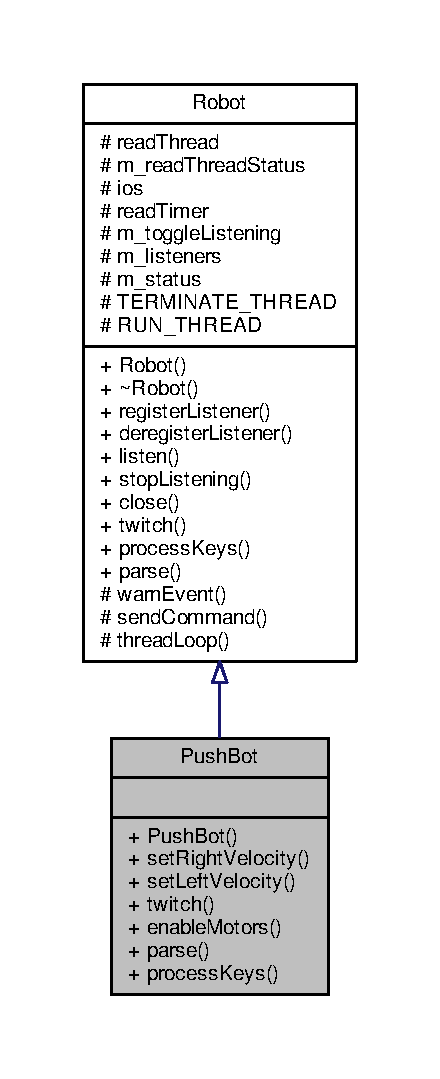
\includegraphics[width=211pt]{class_push_bot__inherit__graph}
\end{center}
\end{figure}


Collaboration diagram for Push\+Bot\+:
\nopagebreak
\begin{figure}[H]
\begin{center}
\leavevmode
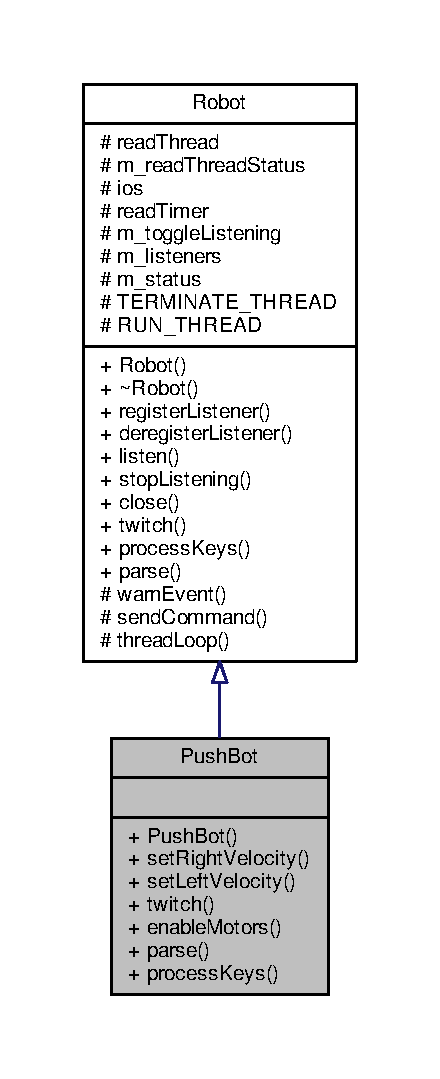
\includegraphics[width=211pt]{class_push_bot__coll__graph}
\end{center}
\end{figure}
\subsection*{Public Member Functions}
\begin{DoxyCompactItemize}
\item 
\hyperlink{class_push_bot_a9f01f2663700a2894c0cb52651ec7a8b}{Push\+Bot} (int file\+Descriptor)
\begin{DoxyCompactList}\small\item\em Constructor. \end{DoxyCompactList}\item 
\hypertarget{class_push_bot_a14e806fd8d5b1757440147099a393b2e}{}bool \hyperlink{class_push_bot_a14e806fd8d5b1757440147099a393b2e}{set\+Right\+Velocity} (int)\label{class_push_bot_a14e806fd8d5b1757440147099a393b2e}

\begin{DoxyCompactList}\small\item\em set the velocity of the right wheel \end{DoxyCompactList}\item 
\hypertarget{class_push_bot_aede73ab503b5732df67126a4322074f6}{}bool \hyperlink{class_push_bot_aede73ab503b5732df67126a4322074f6}{set\+Left\+Velocity} (int)\label{class_push_bot_aede73ab503b5732df67126a4322074f6}

\begin{DoxyCompactList}\small\item\em set the velocity of the left wheel \end{DoxyCompactList}\item 
\hypertarget{class_push_bot_aeac29d4529c93c2cabbfaab4a7358480}{}bool \hyperlink{class_push_bot_aeac29d4529c93c2cabbfaab4a7358480}{twitch} ()\label{class_push_bot_aeac29d4529c93c2cabbfaab4a7358480}

\begin{DoxyCompactList}\small\item\em check if the servos are working \end{DoxyCompactList}\item 
\hypertarget{class_push_bot_a55ab1fbdf79449dd45cc1d666da9e607}{}bool \hyperlink{class_push_bot_a55ab1fbdf79449dd45cc1d666da9e607}{enable\+Motors} ()\label{class_push_bot_a55ab1fbdf79449dd45cc1d666da9e607}

\begin{DoxyCompactList}\small\item\em start the motors up \end{DoxyCompactList}\item 
\hypertarget{class_push_bot_ae5ebe6028f68a35849a5d7802a1c154e}{}void \hyperlink{class_push_bot_ae5ebe6028f68a35849a5d7802a1c154e}{parse} (unsigned char $\ast$, int)\label{class_push_bot_ae5ebe6028f68a35849a5d7802a1c154e}

\begin{DoxyCompactList}\small\item\em parse message \end{DoxyCompactList}\item 
\hypertarget{class_push_bot_a9d898a09d60c5f8c34f8fd437c5d3b24}{}void \hyperlink{class_push_bot_a9d898a09d60c5f8c34f8fd437c5d3b24}{process\+Keys} (int keys\+Pressed)\label{class_push_bot_a9d898a09d60c5f8c34f8fd437c5d3b24}

\begin{DoxyCompactList}\small\item\em process key strokes logged from the keyboard \end{DoxyCompactList}\end{DoxyCompactItemize}
\subsection*{Additional Inherited Members}


\subsection{Detailed Description}
Mid-\/\+Level interface to the \hyperlink{class_push_bot}{Push\+Bot}. Communnication via Wi\+Fi. 

\subsection{Constructor \& Destructor Documentation}
\hypertarget{class_push_bot_a9f01f2663700a2894c0cb52651ec7a8b}{}\index{Push\+Bot@{Push\+Bot}!Push\+Bot@{Push\+Bot}}
\index{Push\+Bot@{Push\+Bot}!Push\+Bot@{Push\+Bot}}
\subsubsection[{Push\+Bot}]{\setlength{\rightskip}{0pt plus 5cm}Push\+Bot\+::\+Push\+Bot (
\begin{DoxyParamCaption}
\item[{int}]{file\+Descriptor}
\end{DoxyParamCaption}
)\hspace{0.3cm}{\ttfamily [inline]}}\label{class_push_bot_a9f01f2663700a2894c0cb52651ec7a8b}


Constructor. 


\begin{DoxyParams}{Parameters}
{\em file\+Descriptor} & file descriptor to a successfully opened socket to the push\+Bot \\
\hline
\end{DoxyParams}


The documentation for this class was generated from the following files\+:\begin{DoxyCompactItemize}
\item 
/home/serge/\+Documents/\+Semester Project I\+N\+I/omnibot-\/lib/\+U\+S\+B\+\_\+robot/include/\hyperlink{_push_bot_8h}{Push\+Bot.\+h}\item 
/home/serge/\+Documents/\+Semester Project I\+N\+I/omnibot-\/lib/\+U\+S\+B\+\_\+robot/src/Push\+Bot.\+cpp\end{DoxyCompactItemize}

\hypertarget{class_robot}{}\section{Robot Class Reference}
\label{class_robot}\index{Robot@{Robot}}


Abstact base class defining the required interface to robot.  




{\ttfamily \#include $<$Robot.\+h$>$}



Inheritance diagram for Robot\+:
\nopagebreak
\begin{figure}[H]
\begin{center}
\leavevmode
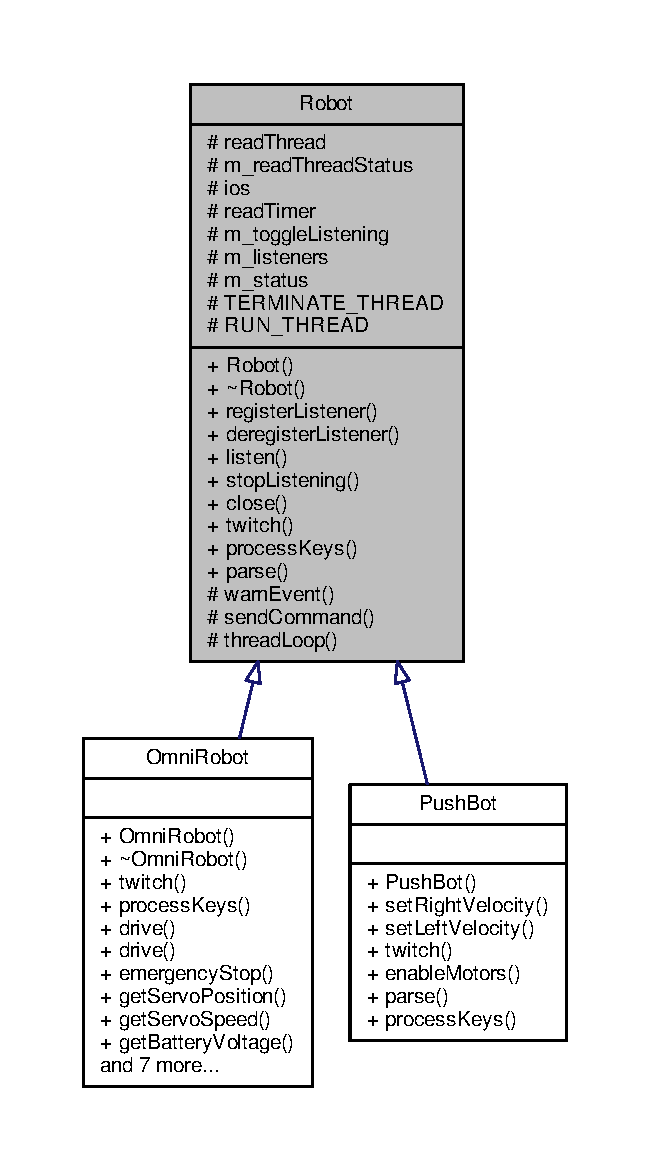
\includegraphics[height=550pt]{class_robot__inherit__graph}
\end{center}
\end{figure}


Collaboration diagram for Robot\+:
\nopagebreak
\begin{figure}[H]
\begin{center}
\leavevmode
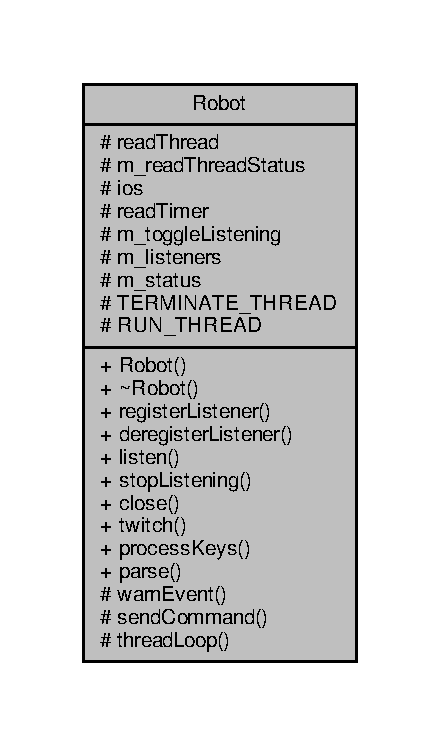
\includegraphics[width=211pt]{class_robot__coll__graph}
\end{center}
\end{figure}
\subsection*{Public Member Functions}
\begin{DoxyCompactItemize}
\item 
\hypertarget{class_robot_aa23c8bfa375d4f817afd7e2f6ae045f0}{}\hyperlink{class_robot_aa23c8bfa375d4f817afd7e2f6ae045f0}{Robot} (int file\+Descriptor)\label{class_robot_aa23c8bfa375d4f817afd7e2f6ae045f0}

\begin{DoxyCompactList}\small\item\em The constructor takes a valid file file descriptor. \end{DoxyCompactList}\item 
\hypertarget{class_robot_adf034063ea4f50ad8bc80dff10c52fbd}{}void \hyperlink{class_robot_adf034063ea4f50ad8bc80dff10c52fbd}{register\+Listener} (\hyperlink{class_robot_listener}{Robot\+Listener} $\ast$)\label{class_robot_adf034063ea4f50ad8bc80dff10c52fbd}

\begin{DoxyCompactList}\small\item\em register a Listener to this robot \end{DoxyCompactList}\item 
\hypertarget{class_robot_a50bfeaa82bcdae08e2b92c1ab0308e9c}{}void \hyperlink{class_robot_a50bfeaa82bcdae08e2b92c1ab0308e9c}{deregister\+Listener} (\hyperlink{class_robot_listener}{Robot\+Listener} $\ast$)\label{class_robot_a50bfeaa82bcdae08e2b92c1ab0308e9c}

\begin{DoxyCompactList}\small\item\em degregister a specific listener \end{DoxyCompactList}\item 
\hypertarget{class_robot_a6713c453dde16f83b1368fce66130228}{}int \hyperlink{class_robot_a6713c453dde16f83b1368fce66130228}{listen} ()\label{class_robot_a6713c453dde16f83b1368fce66130228}

\begin{DoxyCompactList}\small\item\em start listening to new events from the data stream received \end{DoxyCompactList}\item 
\hypertarget{class_robot_ad0dc163ea28c82cb52ed53e9da913368}{}int \hyperlink{class_robot_ad0dc163ea28c82cb52ed53e9da913368}{stop\+Listening} ()\label{class_robot_ad0dc163ea28c82cb52ed53e9da913368}

\begin{DoxyCompactList}\small\item\em stop listening \end{DoxyCompactList}\item 
\hypertarget{class_robot_a091253a377e3f6944616ee0f0fad8941}{}int \hyperlink{class_robot_a091253a377e3f6944616ee0f0fad8941}{close} ()\label{class_robot_a091253a377e3f6944616ee0f0fad8941}

\begin{DoxyCompactList}\small\item\em close the serial port \end{DoxyCompactList}\item 
\hypertarget{class_robot_a89c1fc16ed3ae6bb3162837b1fbf689a}{}virtual bool \hyperlink{class_robot_a89c1fc16ed3ae6bb3162837b1fbf689a}{twitch} ()=0\label{class_robot_a89c1fc16ed3ae6bb3162837b1fbf689a}

\begin{DoxyCompactList}\small\item\em check the robot when starting up \end{DoxyCompactList}\item 
\hypertarget{class_robot_ac09d08242ccbdd6c4bc68bfe689759f0}{}virtual void \hyperlink{class_robot_ac09d08242ccbdd6c4bc68bfe689759f0}{process\+Keys} (int keys\+Pressed)=0\label{class_robot_ac09d08242ccbdd6c4bc68bfe689759f0}

\begin{DoxyCompactList}\small\item\em process logged keystrokes and triggers the required action \end{DoxyCompactList}\item 
\hypertarget{class_robot_a7dcc9de1f4a64894bdc047efd5db8a2b}{}virtual void \hyperlink{class_robot_a7dcc9de1f4a64894bdc047efd5db8a2b}{parse} (unsigned char $\ast$data, int bytes\+Read)=0\label{class_robot_a7dcc9de1f4a64894bdc047efd5db8a2b}

\begin{DoxyCompactList}\small\item\em Parses the commands of interest from the input. \end{DoxyCompactList}\end{DoxyCompactItemize}
\subsection*{Protected Member Functions}
\begin{DoxyCompactItemize}
\item 
\hypertarget{class_robot_a394e0a75b695970a8d67edb86d9c6b57}{}void \hyperlink{class_robot_a394e0a75b695970a8d67edb86d9c6b57}{warn\+Event} (std\+::queue$<$ \hyperlink{structservo_signals}{servo\+Signals} $>$ \&, std\+::queue$<$ \hyperlink{structbumper}{bumper} $>$ \&)\label{class_robot_a394e0a75b695970a8d67edb86d9c6b57}

\begin{DoxyCompactList}\small\item\em Notifies all the registered listeners that an event has occured. \end{DoxyCompactList}\item 
\hypertarget{class_robot_a55d36d87b7b3826fc5f495359c5472fd}{}int \hyperlink{class_robot_a55d36d87b7b3826fc5f495359c5472fd}{send\+Command} (std\+::string cmd)\label{class_robot_a55d36d87b7b3826fc5f495359c5472fd}

\begin{DoxyCompactList}\small\item\em send a command to the device, is the same for a serial or a T\+C\+P device \end{DoxyCompactList}\end{DoxyCompactItemize}
\subsection*{Static Protected Member Functions}
\begin{DoxyCompactItemize}
\item 
\hypertarget{class_robot_af159507f5d8069107a54fd31965cb65d}{}static void {\bfseries thread\+Loop} (boost\+::asio\+::deadline\+\_\+timer $\ast$, int $\ast$, void $\ast$)\label{class_robot_af159507f5d8069107a54fd31965cb65d}

\end{DoxyCompactItemize}
\subsection*{Protected Attributes}
\begin{DoxyCompactItemize}
\item 
\hypertarget{class_robot_a7f81941312c87b38ef5c60f02d565bcb}{}boost\+::thread $\ast$ {\bfseries read\+Thread}\label{class_robot_a7f81941312c87b38ef5c60f02d565bcb}

\item 
\hypertarget{class_robot_ac6e92828eb711facd7fe88fa9e80961c}{}int {\bfseries m\+\_\+read\+Thread\+Status}\label{class_robot_ac6e92828eb711facd7fe88fa9e80961c}

\item 
\hypertarget{class_robot_aa8835ee41157aeab028a0aaeff133890}{}boost\+::asio\+::io\+\_\+service $\ast$ {\bfseries ios}\label{class_robot_aa8835ee41157aeab028a0aaeff133890}

\item 
\hypertarget{class_robot_a1adb110a11b739f6627dcf4ca8798817}{}boost\+::asio\+::deadline\+\_\+timer $\ast$ {\bfseries read\+Timer}\label{class_robot_a1adb110a11b739f6627dcf4ca8798817}

\item 
\hypertarget{class_robot_a379696f4a6eb66246569e3833fc2f271}{}bool {\bfseries m\+\_\+toggle\+Listening}\label{class_robot_a379696f4a6eb66246569e3833fc2f271}

\item 
\hypertarget{class_robot_a7c1c1ec2aa764902fe2cbe814f612df9}{}std\+::list$<$ \hyperlink{class_robot_listener}{Robot\+Listener} $\ast$ $>$ \hyperlink{class_robot_a7c1c1ec2aa764902fe2cbe814f612df9}{m\+\_\+listeners}\label{class_robot_a7c1c1ec2aa764902fe2cbe814f612df9}

\begin{DoxyCompactList}\small\item\em Registered listeners. \end{DoxyCompactList}\item 
\hypertarget{class_robot_aefb0abbfc6681d039e188892c137d689}{}int {\bfseries m\+\_\+status}\label{class_robot_aefb0abbfc6681d039e188892c137d689}

\end{DoxyCompactItemize}
\subsection*{Static Protected Attributes}
\begin{DoxyCompactItemize}
\item 
\hypertarget{class_robot_af6a64b83d24e0f46636946e9a0a0ccd3}{}static const int {\bfseries T\+E\+R\+M\+I\+N\+A\+T\+E\+\_\+\+T\+H\+R\+E\+A\+D} = -\/1\label{class_robot_af6a64b83d24e0f46636946e9a0a0ccd3}

\item 
\hypertarget{class_robot_a30926b9d988efb171a32cb1855bfa594}{}static const int {\bfseries R\+U\+N\+\_\+\+T\+H\+R\+E\+A\+D} = 1\label{class_robot_a30926b9d988efb171a32cb1855bfa594}

\end{DoxyCompactItemize}


\subsection{Detailed Description}
Abstact base class defining the required interface to robot. 

The documentation for this class was generated from the following files\+:\begin{DoxyCompactItemize}
\item 
/home/serge/\+Documents/\+Semester Project I\+N\+I/omnibot-\/lib/\+U\+S\+B\+\_\+robot/include/Robot.\+h\item 
/home/serge/\+Documents/\+Semester Project I\+N\+I/omnibot-\/lib/\+U\+S\+B\+\_\+robot/src/Robot.\+cpp\end{DoxyCompactItemize}

\hypertarget{structrobot_drive_parameters}{}\section{robot\+Drive\+Parameters Struct Reference}
\label{structrobot_drive_parameters}\index{robot\+Drive\+Parameters@{robot\+Drive\+Parameters}}


Collaboration diagram for robot\+Drive\+Parameters\+:
\nopagebreak
\begin{figure}[H]
\begin{center}
\leavevmode
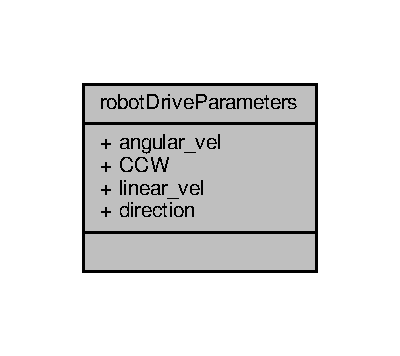
\includegraphics[width=192pt]{structrobot_drive_parameters__coll__graph}
\end{center}
\end{figure}
\subsection*{Public Attributes}
\begin{DoxyCompactItemize}
\item 
\hypertarget{structrobot_drive_parameters_a2b64928c6867161fa4e01e38983887a2}{}double {\bfseries angular\+\_\+vel}\label{structrobot_drive_parameters_a2b64928c6867161fa4e01e38983887a2}

\item 
\hypertarget{structrobot_drive_parameters_ab77a28e264d1f1b2372cca0658f027f4}{}bool {\bfseries C\+C\+W}\label{structrobot_drive_parameters_ab77a28e264d1f1b2372cca0658f027f4}

\item 
\hypertarget{structrobot_drive_parameters_a5dd169a5b0c88a2016fd8cd597474be1}{}double {\bfseries linear\+\_\+vel}\label{structrobot_drive_parameters_a5dd169a5b0c88a2016fd8cd597474be1}

\item 
\hypertarget{structrobot_drive_parameters_ad1a4776988a48cc58fdd71e2eb8447fe}{}double {\bfseries direction}\label{structrobot_drive_parameters_ad1a4776988a48cc58fdd71e2eb8447fe}

\end{DoxyCompactItemize}


The documentation for this struct was generated from the following file\+:\begin{DoxyCompactItemize}
\item 
/home/serge/\+Documents/\+Semester Project I\+N\+I/omnibot-\/lib/\+U\+S\+B\+\_\+robot/include/\hyperlink{my_keyboard_listener_8h}{my\+Keyboard\+Listener.\+h}\end{DoxyCompactItemize}

\hypertarget{structrobot_drive_state}{}\section{robot\+Drive\+State Struct Reference}
\label{structrobot_drive_state}\index{robot\+Drive\+State@{robot\+Drive\+State}}


encapsulates the mid-\/level robot drive parameters  




{\ttfamily \#include $<$Omni\+Robot.\+h$>$}



Collaboration diagram for robot\+Drive\+State\+:
\nopagebreak
\begin{figure}[H]
\begin{center}
\leavevmode
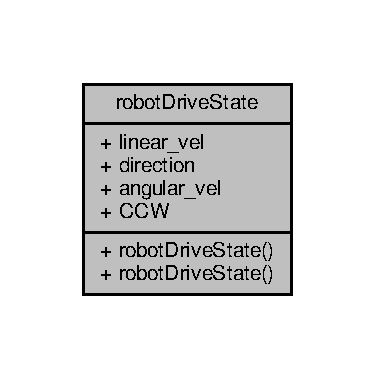
\includegraphics[width=180pt]{structrobot_drive_state__coll__graph}
\end{center}
\end{figure}
\subsection*{Public Member Functions}
\begin{DoxyCompactItemize}
\item 
\hypertarget{structrobot_drive_state_a731efd107a95b59c58e850702a9f6277}{}{\bfseries robot\+Drive\+State} (double an\+Angular\+Vel, bool a\+C\+C\+W, double a\+Lin\+Vel, double a\+Direction)\label{structrobot_drive_state_a731efd107a95b59c58e850702a9f6277}

\end{DoxyCompactItemize}
\subsection*{Public Attributes}
\begin{DoxyCompactItemize}
\item 
\hypertarget{structrobot_drive_state_add7fd9cb9f3093995d3179e0d23f89e1}{}double \hyperlink{structrobot_drive_state_add7fd9cb9f3093995d3179e0d23f89e1}{linear\+\_\+vel}\label{structrobot_drive_state_add7fd9cb9f3093995d3179e0d23f89e1}

\begin{DoxyCompactList}\small\item\em Linear velocity of the robot. \end{DoxyCompactList}\item 
\hypertarget{structrobot_drive_state_a117f5c632459517d549ee5e9ecaaa008}{}double \hyperlink{structrobot_drive_state_a117f5c632459517d549ee5e9ecaaa008}{direction}\label{structrobot_drive_state_a117f5c632459517d549ee5e9ecaaa008}

\begin{DoxyCompactList}\small\item\em The directio the robot is headed with respect to its initial position. \end{DoxyCompactList}\item 
\hypertarget{structrobot_drive_state_aaddce997ec0bc7495e60cf577b956af7}{}double \hyperlink{structrobot_drive_state_aaddce997ec0bc7495e60cf577b956af7}{angular\+\_\+vel}\label{structrobot_drive_state_aaddce997ec0bc7495e60cf577b956af7}

\begin{DoxyCompactList}\small\item\em The angular velocity of the robot. \end{DoxyCompactList}\item 
\hypertarget{structrobot_drive_state_a0e604f06f3708dacbfd81105fa135053}{}bool \hyperlink{structrobot_drive_state_a0e604f06f3708dacbfd81105fa135053}{C\+C\+W}\label{structrobot_drive_state_a0e604f06f3708dacbfd81105fa135053}

\begin{DoxyCompactList}\small\item\em Truning direction of the robot. \end{DoxyCompactList}\end{DoxyCompactItemize}


\subsection{Detailed Description}
encapsulates the mid-\/level robot drive parameters 

The documentation for this struct was generated from the following file\+:\begin{DoxyCompactItemize}
\item 
/home/serge/\+Documents/\+Semester Project I\+N\+I/omnibot-\/lib/\+U\+S\+B\+\_\+robot/include/\hyperlink{_omni_robot_8h}{Omni\+Robot.\+h}\end{DoxyCompactItemize}

\hypertarget{class_robot_listener}{}\section{Robot\+Listener Class Reference}
\label{class_robot_listener}\index{Robot\+Listener@{Robot\+Listener}}


Abstarct base class providing the necessary interface to observe the servo states and bumper states of the observed robot.  




{\ttfamily \#include $<$Robot\+Listener.\+h$>$}



Inheritance diagram for Robot\+Listener\+:
\nopagebreak
\begin{figure}[H]
\begin{center}
\leavevmode
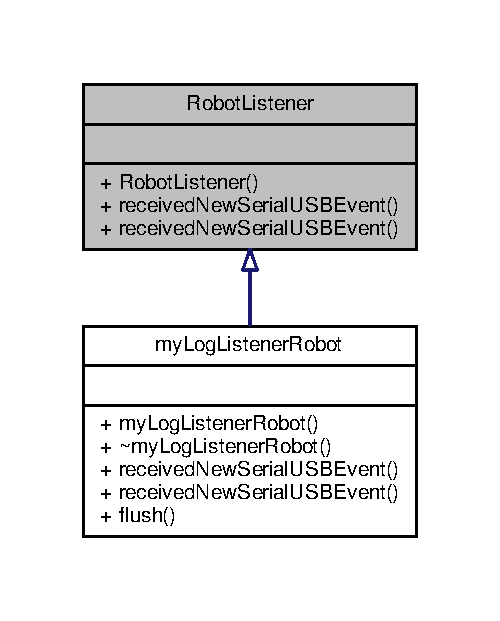
\includegraphics[width=240pt]{class_robot_listener__inherit__graph}
\end{center}
\end{figure}


Collaboration diagram for Robot\+Listener\+:
\nopagebreak
\begin{figure}[H]
\begin{center}
\leavevmode
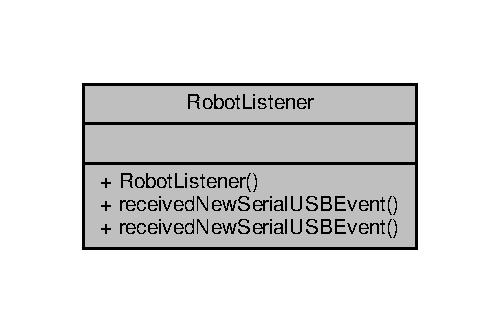
\includegraphics[width=240pt]{class_robot_listener__coll__graph}
\end{center}
\end{figure}
\subsection*{Public Member Functions}
\begin{DoxyCompactItemize}
\item 
\hypertarget{class_robot_listener_af6be6176f19b4bd28edee8893211a8b2}{}virtual void \hyperlink{class_robot_listener_af6be6176f19b4bd28edee8893211a8b2}{received\+New\+Serial\+U\+S\+B\+Event} (std\+::queue$<$ \hyperlink{structservo_signals}{servo\+Signals} $>$ \&)=0\label{class_robot_listener_af6be6176f19b4bd28edee8893211a8b2}

\begin{DoxyCompactList}\small\item\em virtual function to receive the decoded servos signals \end{DoxyCompactList}\item 
\hypertarget{class_robot_listener_a73f24d40ff4a0bf93942f2bf261e186c}{}virtual void \hyperlink{class_robot_listener_a73f24d40ff4a0bf93942f2bf261e186c}{received\+New\+Serial\+U\+S\+B\+Event} (std\+::queue$<$ \hyperlink{structbumper}{bumper} $>$ \&)=0\label{class_robot_listener_a73f24d40ff4a0bf93942f2bf261e186c}

\begin{DoxyCompactList}\small\item\em virtual function to receive the decoded bumper events \end{DoxyCompactList}\end{DoxyCompactItemize}


\subsection{Detailed Description}
Abstarct base class providing the necessary interface to observe the servo states and bumper states of the observed robot. 

This class needs to be subcalssed and the member functions need to be implemented in order to use the interface 

The documentation for this class was generated from the following file\+:\begin{DoxyCompactItemize}
\item 
/home/serge/\+Documents/\+Semester Project I\+N\+I/omnibot-\/lib/\+U\+S\+B\+\_\+robot/include/\hyperlink{_robot_listener_8h}{Robot\+Listener.\+h}\end{DoxyCompactItemize}

\hypertarget{structservo_signals}{}\section{servo\+Signals Struct Reference}
\label{structservo_signals}\index{servo\+Signals@{servo\+Signals}}


Collaboration diagram for servo\+Signals\+:
\nopagebreak
\begin{figure}[H]
\begin{center}
\leavevmode
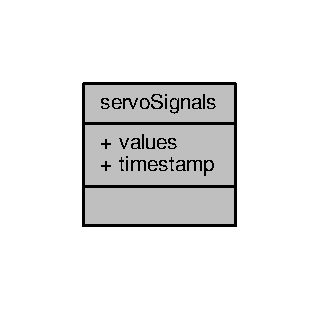
\includegraphics[width=153pt]{structservo_signals__coll__graph}
\end{center}
\end{figure}
\subsection*{Public Attributes}
\begin{DoxyCompactItemize}
\item 
\hypertarget{structservo_signals_a0ed5b965b518f964a9a63f432d142a5b}{}int {\bfseries values} \mbox{[}3\mbox{]}\label{structservo_signals_a0ed5b965b518f964a9a63f432d142a5b}

\item 
\hypertarget{structservo_signals_ad8060d17bc7e15051080dfb5f504b061}{}std\+::string {\bfseries timestamp}\label{structservo_signals_ad8060d17bc7e15051080dfb5f504b061}

\end{DoxyCompactItemize}


The documentation for this struct was generated from the following file\+:\begin{DoxyCompactItemize}
\item 
/home/serge/\+Documents/\+Semester Project I\+N\+I/omnibot-\/lib/\+U\+S\+B\+\_\+robot/include/\hyperlink{_robot_listener_8h}{Robot\+Listener.\+h}\end{DoxyCompactItemize}

\chapter{File Documentation}
\hypertarget{_e_b_v___e_d_v_s4337_serial_u_s_b_8h}{}\section{/home/serge/\+Documents/\+Semester Project I\+N\+I/omnibot-\/lib/\+U\+S\+B\+\_\+robot/include/\+E\+B\+V\+\_\+\+E\+D\+V\+S4337\+Serial\+U\+S\+B.h File Reference}
\label{_e_b_v___e_d_v_s4337_serial_u_s_b_8h}\index{/home/serge/\+Documents/\+Semester Project I\+N\+I/omnibot-\/lib/\+U\+S\+B\+\_\+robot/include/\+E\+B\+V\+\_\+\+E\+D\+V\+S4337\+Serial\+U\+S\+B.\+h@{/home/serge/\+Documents/\+Semester Project I\+N\+I/omnibot-\/lib/\+U\+S\+B\+\_\+robot/include/\+E\+B\+V\+\_\+\+E\+D\+V\+S4337\+Serial\+U\+S\+B.\+h}}


provides the necessary interface for communication and listening to the e\+D\+V\+S camera and the embedded I\+M\+U  


{\ttfamily \#include $<$stdio.\+h$>$}\\*
{\ttfamily \#include $<$termios.\+h$>$}\\*
{\ttfamily \#include $<$string$>$}\\*
{\ttfamily \#include $<$vector$>$}\\*
{\ttfamily \#include $<$list$>$}\\*
{\ttfamily \#include $<$Log\+Wrapper.\+h$>$}\\*
Include dependency graph for E\+B\+V\+\_\+\+E\+D\+V\+S4337\+Serial\+U\+S\+B.\+h\+:\nopagebreak
\begin{figure}[H]
\begin{center}
\leavevmode
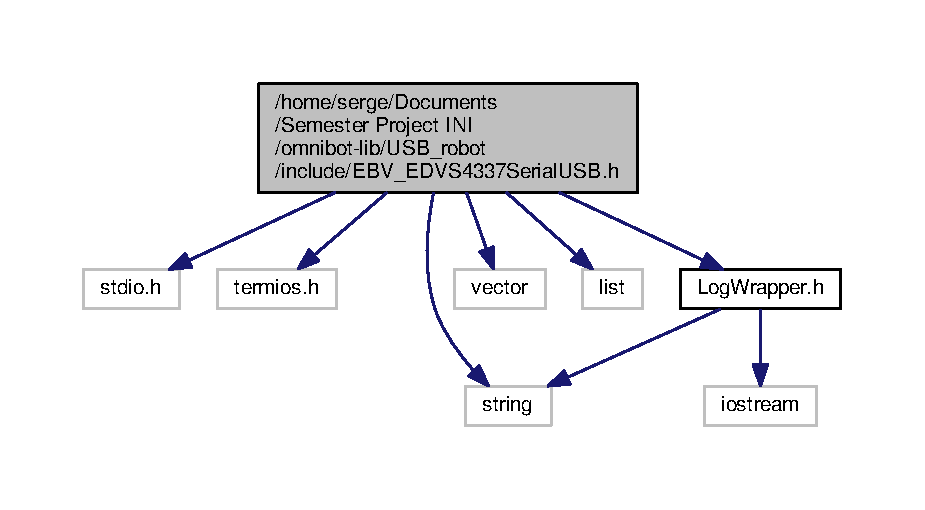
\includegraphics[width=350pt]{_e_b_v___e_d_v_s4337_serial_u_s_b_8h__incl}
\end{center}
\end{figure}
This graph shows which files directly or indirectly include this file\+:\nopagebreak
\begin{figure}[H]
\begin{center}
\leavevmode
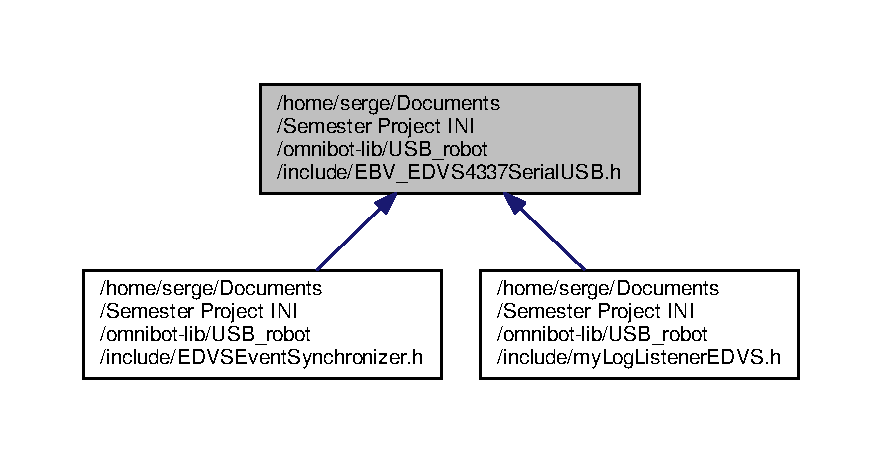
\includegraphics[width=350pt]{_e_b_v___e_d_v_s4337_serial_u_s_b_8h__dep__incl}
\end{center}
\end{figure}
\subsection*{Classes}
\begin{DoxyCompactItemize}
\item 
class \hyperlink{struct_e_d_v_s4337_serial_u_s_b_event}{E\+D\+V\+S4337\+Serial\+U\+S\+B\+Event}
\begin{DoxyCompactList}\small\item\em encapsulates the camera events parsed from the event stream coming from the e\+D\+V\+S. \end{DoxyCompactList}\item 
class \hyperlink{struct_e_d_v_s4337_serial_u_s_b_i_m_u_event}{E\+D\+V\+S4337\+Serial\+U\+S\+B\+I\+M\+U\+Event}
\begin{DoxyCompactList}\small\item\em encapsulates the I\+M\+U events parsed from the event stream coming from the e\+D\+V\+S. \end{DoxyCompactList}\item 
struct \hyperlink{struct_e_d_v_s4337_serial_u_s_b_biases}{E\+D\+V\+S4337\+Serial\+U\+S\+B\+Biases}
\begin{DoxyCompactList}\small\item\em encapsulates the values for the biases and stores them in an array with the help of the biases\+\_\+t enum for better readability. \end{DoxyCompactList}\item 
class \hyperlink{class_e_d_v_s4337_serial_u_s_b_listener}{E\+D\+V\+S4337\+Serial\+U\+S\+B\+Listener}
\begin{DoxyCompactList}\small\item\em abstract base class for a listener that observers e\+D\+V\+S events \end{DoxyCompactList}\item 
class \hyperlink{class_e_d_v_s4337_serial_u_s_b_i_m_u_listener}{E\+D\+V\+S4337\+Serial\+U\+S\+B\+I\+M\+U\+Listener}
\begin{DoxyCompactList}\small\item\em abstract base class for a listener that observers I\+M\+U events \end{DoxyCompactList}\item 
struct \hyperlink{struct_e_d_v_s4337_serial_u_s_b_args}{E\+D\+V\+S4337\+Serial\+U\+S\+B\+Args}
\begin{DoxyCompactList}\small\item\em encapsulates the necessary arguments to start reading from the serial port in a new Threading \end{DoxyCompactList}\item 
class \hyperlink{class_e_d_v_s4337_serial_u_s_b}{E\+D\+V\+S4337\+Serial\+U\+S\+B}
\begin{DoxyCompactList}\small\item\em Class providing the necessary interfaces for communication and event streaming from the e\+D\+V\+S camera. \end{DoxyCompactList}\end{DoxyCompactItemize}
\subsection*{Enumerations}
\begin{DoxyCompactItemize}
\item 
enum \hyperlink{_e_b_v___e_d_v_s4337_serial_u_s_b_8h_a0580b5f9d6ec67f7bb47b4f52cff0cfd}{biases\+\_\+t} \{ \\*
\hyperlink{_e_b_v___e_d_v_s4337_serial_u_s_b_8h_a0580b5f9d6ec67f7bb47b4f52cff0cfdab1ff1fca6e9f99e11dd50c90b79b003e}{C\+A\+S}, 
\hyperlink{_e_b_v___e_d_v_s4337_serial_u_s_b_8h_a0580b5f9d6ec67f7bb47b4f52cff0cfda5e94bdfd0950671d324a2b2bf66bc870}{I\+N\+J\+\_\+\+G\+N\+D}, 
\hyperlink{_e_b_v___e_d_v_s4337_serial_u_s_b_8h_a0580b5f9d6ec67f7bb47b4f52cff0cfdad6fa580bd5459cac89665a87b806a9ed}{R\+E\+Q\+\_\+\+P\+D}, 
\hyperlink{_e_b_v___e_d_v_s4337_serial_u_s_b_8h_a0580b5f9d6ec67f7bb47b4f52cff0cfda0accf91ca0b9dae6110871c69587921f}{P\+U\+\_\+\+X}, 
\\*
\hyperlink{_e_b_v___e_d_v_s4337_serial_u_s_b_8h_a0580b5f9d6ec67f7bb47b4f52cff0cfdaea81793d8e8675252e00fd9f4c5d3cf0}{D\+I\+F\+F\+\_\+\+O\+F\+F}, 
\hyperlink{_e_b_v___e_d_v_s4337_serial_u_s_b_8h_a0580b5f9d6ec67f7bb47b4f52cff0cfdab64fee4faebf865dbe5c0a5c444a0fa3}{R\+E\+Q}, 
\hyperlink{_e_b_v___e_d_v_s4337_serial_u_s_b_8h_a0580b5f9d6ec67f7bb47b4f52cff0cfda3d5742d3e7cd7a959af35fe0a3def065}{R\+E\+F\+R}, 
\hyperlink{_e_b_v___e_d_v_s4337_serial_u_s_b_8h_a0580b5f9d6ec67f7bb47b4f52cff0cfda06d6d56211d52afc38dcab004b37a0b5}{P\+U\+\_\+\+Y}, 
\\*
\hyperlink{_e_b_v___e_d_v_s4337_serial_u_s_b_8h_a0580b5f9d6ec67f7bb47b4f52cff0cfdaf0c8bbff2a26f14a7a49d910174d0501}{D\+I\+F\+F\+\_\+\+O\+N}, 
\hyperlink{_e_b_v___e_d_v_s4337_serial_u_s_b_8h_a0580b5f9d6ec67f7bb47b4f52cff0cfdaa5d305f703cfce63b982a4cba74f64ec}{D\+I\+F\+F}, 
\hyperlink{_e_b_v___e_d_v_s4337_serial_u_s_b_8h_a0580b5f9d6ec67f7bb47b4f52cff0cfda24e93623f9d4a47c59ab2bd5f063ce47}{F\+O\+L\+L}, 
\hyperlink{_e_b_v___e_d_v_s4337_serial_u_s_b_8h_a0580b5f9d6ec67f7bb47b4f52cff0cfda9c17aec256007f966da3c8dabfd5bcb8}{P\+R}
 \}
\begin{DoxyCompactList}\small\item\em defines the biases necessary for proper e\+D\+V\+S initialization \end{DoxyCompactList}\item 
enum \hyperlink{_e_b_v___e_d_v_s4337_serial_u_s_b_8h_a2b0bc356728b430ea3809f44d9be46c1}{Event\+Format} \{ \\*
\hyperlink{_e_b_v___e_d_v_s4337_serial_u_s_b_8h_a2b0bc356728b430ea3809f44d9be46c1ac1bb60616b27745112e0ee86c7b09a14}{E\+V\+T\+\_\+\+F\+O\+R\+M\+A\+T\+\_\+\+E0}, 
\hyperlink{_e_b_v___e_d_v_s4337_serial_u_s_b_8h_a2b0bc356728b430ea3809f44d9be46c1a0ee9623f1f89fac7e52b79b021603a19}{E\+V\+T\+\_\+\+F\+O\+R\+M\+A\+T\+\_\+\+E1}, 
\hyperlink{_e_b_v___e_d_v_s4337_serial_u_s_b_8h_a2b0bc356728b430ea3809f44d9be46c1aa4df9541c0c1b3cb55aa9fe9b6d35397}{E\+V\+T\+\_\+\+F\+O\+R\+M\+A\+T\+\_\+\+E2}, 
\hyperlink{_e_b_v___e_d_v_s4337_serial_u_s_b_8h_a2b0bc356728b430ea3809f44d9be46c1ae27a60feed3cbdfe6e68ac2e02e787f5}{E\+V\+T\+\_\+\+F\+O\+R\+M\+A\+T\+\_\+\+E3}, 
\\*
\hyperlink{_e_b_v___e_d_v_s4337_serial_u_s_b_8h_a2b0bc356728b430ea3809f44d9be46c1a8bb2de3763cc82614e6785daad63e7e6}{E\+V\+T\+\_\+\+F\+O\+R\+M\+A\+T\+\_\+\+E4}
 \}
\begin{DoxyCompactList}\small\item\em provides all the event formats that are supported by this camers. \end{DoxyCompactList}\end{DoxyCompactItemize}


\subsection{Detailed Description}
provides the necessary interface for communication and listening to the e\+D\+V\+S camera and the embedded I\+M\+U 



\subsection{Enumeration Type Documentation}
\hypertarget{_e_b_v___e_d_v_s4337_serial_u_s_b_8h_a0580b5f9d6ec67f7bb47b4f52cff0cfd}{}\index{E\+B\+V\+\_\+\+E\+D\+V\+S4337\+Serial\+U\+S\+B.\+h@{E\+B\+V\+\_\+\+E\+D\+V\+S4337\+Serial\+U\+S\+B.\+h}!biases\+\_\+t@{biases\+\_\+t}}
\index{biases\+\_\+t@{biases\+\_\+t}!E\+B\+V\+\_\+\+E\+D\+V\+S4337\+Serial\+U\+S\+B.\+h@{E\+B\+V\+\_\+\+E\+D\+V\+S4337\+Serial\+U\+S\+B.\+h}}
\subsubsection[{biases\+\_\+t}]{\setlength{\rightskip}{0pt plus 5cm}enum {\bf biases\+\_\+t}}\label{_e_b_v___e_d_v_s4337_serial_u_s_b_8h_a0580b5f9d6ec67f7bb47b4f52cff0cfd}


defines the biases necessary for proper e\+D\+V\+S initialization 

\begin{DoxySeeAlso}{See also}
here for more information\+: \href{http://inilabs.com/support/hardware/biasing/#h.khgrv1ecqm5q}{\tt http\+://inilabs.\+com/support/hardware/biasing/\#h.\+khgrv1ecqm5q} 
\end{DoxySeeAlso}
\begin{Desc}
\item[Enumerator]\par
\begin{description}
\index{C\+A\+S@{C\+A\+S}!E\+B\+V\+\_\+\+E\+D\+V\+S4337\+Serial\+U\+S\+B.\+h@{E\+B\+V\+\_\+\+E\+D\+V\+S4337\+Serial\+U\+S\+B.\+h}}\index{E\+B\+V\+\_\+\+E\+D\+V\+S4337\+Serial\+U\+S\+B.\+h@{E\+B\+V\+\_\+\+E\+D\+V\+S4337\+Serial\+U\+S\+B.\+h}!C\+A\+S@{C\+A\+S}}\item[{\em 
\hypertarget{_e_b_v___e_d_v_s4337_serial_u_s_b_8h_a0580b5f9d6ec67f7bb47b4f52cff0cfdab1ff1fca6e9f99e11dd50c90b79b003e}{}C\+A\+S\label{_e_b_v___e_d_v_s4337_serial_u_s_b_8h_a0580b5f9d6ec67f7bb47b4f52cff0cfdab1ff1fca6e9f99e11dd50c90b79b003e}
}]First stage cascode. \index{I\+N\+J\+\_\+\+G\+N\+D@{I\+N\+J\+\_\+\+G\+N\+D}!E\+B\+V\+\_\+\+E\+D\+V\+S4337\+Serial\+U\+S\+B.\+h@{E\+B\+V\+\_\+\+E\+D\+V\+S4337\+Serial\+U\+S\+B.\+h}}\index{E\+B\+V\+\_\+\+E\+D\+V\+S4337\+Serial\+U\+S\+B.\+h@{E\+B\+V\+\_\+\+E\+D\+V\+S4337\+Serial\+U\+S\+B.\+h}!I\+N\+J\+\_\+\+G\+N\+D@{I\+N\+J\+\_\+\+G\+N\+D}}\item[{\em 
\hypertarget{_e_b_v___e_d_v_s4337_serial_u_s_b_8h_a0580b5f9d6ec67f7bb47b4f52cff0cfda5e94bdfd0950671d324a2b2bf66bc870}{}I\+N\+J\+\_\+\+G\+N\+D\label{_e_b_v___e_d_v_s4337_serial_u_s_b_8h_a0580b5f9d6ec67f7bb47b4f52cff0cfda5e94bdfd0950671d324a2b2bf66bc870}
}]Injected ground. \index{R\+E\+Q\+\_\+\+P\+D@{R\+E\+Q\+\_\+\+P\+D}!E\+B\+V\+\_\+\+E\+D\+V\+S4337\+Serial\+U\+S\+B.\+h@{E\+B\+V\+\_\+\+E\+D\+V\+S4337\+Serial\+U\+S\+B.\+h}}\index{E\+B\+V\+\_\+\+E\+D\+V\+S4337\+Serial\+U\+S\+B.\+h@{E\+B\+V\+\_\+\+E\+D\+V\+S4337\+Serial\+U\+S\+B.\+h}!R\+E\+Q\+\_\+\+P\+D@{R\+E\+Q\+\_\+\+P\+D}}\item[{\em 
\hypertarget{_e_b_v___e_d_v_s4337_serial_u_s_b_8h_a0580b5f9d6ec67f7bb47b4f52cff0cfdad6fa580bd5459cac89665a87b806a9ed}{}R\+E\+Q\+\_\+\+P\+D\label{_e_b_v___e_d_v_s4337_serial_u_s_b_8h_a0580b5f9d6ec67f7bb47b4f52cff0cfdad6fa580bd5459cac89665a87b806a9ed}
}]Pull down on chip request. \index{P\+U\+\_\+\+X@{P\+U\+\_\+\+X}!E\+B\+V\+\_\+\+E\+D\+V\+S4337\+Serial\+U\+S\+B.\+h@{E\+B\+V\+\_\+\+E\+D\+V\+S4337\+Serial\+U\+S\+B.\+h}}\index{E\+B\+V\+\_\+\+E\+D\+V\+S4337\+Serial\+U\+S\+B.\+h@{E\+B\+V\+\_\+\+E\+D\+V\+S4337\+Serial\+U\+S\+B.\+h}!P\+U\+\_\+\+X@{P\+U\+\_\+\+X}}\item[{\em 
\hypertarget{_e_b_v___e_d_v_s4337_serial_u_s_b_8h_a0580b5f9d6ec67f7bb47b4f52cff0cfda0accf91ca0b9dae6110871c69587921f}{}P\+U\+\_\+\+X\label{_e_b_v___e_d_v_s4337_serial_u_s_b_8h_a0580b5f9d6ec67f7bb47b4f52cff0cfda0accf91ca0b9dae6110871c69587921f}
}]Pull up on request from X arbiter. \index{D\+I\+F\+F\+\_\+\+O\+F\+F@{D\+I\+F\+F\+\_\+\+O\+F\+F}!E\+B\+V\+\_\+\+E\+D\+V\+S4337\+Serial\+U\+S\+B.\+h@{E\+B\+V\+\_\+\+E\+D\+V\+S4337\+Serial\+U\+S\+B.\+h}}\index{E\+B\+V\+\_\+\+E\+D\+V\+S4337\+Serial\+U\+S\+B.\+h@{E\+B\+V\+\_\+\+E\+D\+V\+S4337\+Serial\+U\+S\+B.\+h}!D\+I\+F\+F\+\_\+\+O\+F\+F@{D\+I\+F\+F\+\_\+\+O\+F\+F}}\item[{\em 
\hypertarget{_e_b_v___e_d_v_s4337_serial_u_s_b_8h_a0580b5f9d6ec67f7bb47b4f52cff0cfdaea81793d8e8675252e00fd9f4c5d3cf0}{}D\+I\+F\+F\+\_\+\+O\+F\+F\label{_e_b_v___e_d_v_s4337_serial_u_s_b_8h_a0580b5f9d6ec67f7bb47b4f52cff0cfdaea81793d8e8675252e00fd9f4c5d3cf0}
}]Threshold for Off events. \index{R\+E\+Q@{R\+E\+Q}!E\+B\+V\+\_\+\+E\+D\+V\+S4337\+Serial\+U\+S\+B.\+h@{E\+B\+V\+\_\+\+E\+D\+V\+S4337\+Serial\+U\+S\+B.\+h}}\index{E\+B\+V\+\_\+\+E\+D\+V\+S4337\+Serial\+U\+S\+B.\+h@{E\+B\+V\+\_\+\+E\+D\+V\+S4337\+Serial\+U\+S\+B.\+h}!R\+E\+Q@{R\+E\+Q}}\item[{\em 
\hypertarget{_e_b_v___e_d_v_s4337_serial_u_s_b_8h_a0580b5f9d6ec67f7bb47b4f52cff0cfdab64fee4faebf865dbe5c0a5c444a0fa3}{}R\+E\+Q\label{_e_b_v___e_d_v_s4337_serial_u_s_b_8h_a0580b5f9d6ec67f7bb47b4f52cff0cfdab64fee4faebf865dbe5c0a5c444a0fa3}
}]Pull down for passive load inverters in digital A\+E\+R pixel circuitry. \index{R\+E\+F\+R@{R\+E\+F\+R}!E\+B\+V\+\_\+\+E\+D\+V\+S4337\+Serial\+U\+S\+B.\+h@{E\+B\+V\+\_\+\+E\+D\+V\+S4337\+Serial\+U\+S\+B.\+h}}\index{E\+B\+V\+\_\+\+E\+D\+V\+S4337\+Serial\+U\+S\+B.\+h@{E\+B\+V\+\_\+\+E\+D\+V\+S4337\+Serial\+U\+S\+B.\+h}!R\+E\+F\+R@{R\+E\+F\+R}}\item[{\em 
\hypertarget{_e_b_v___e_d_v_s4337_serial_u_s_b_8h_a0580b5f9d6ec67f7bb47b4f52cff0cfda3d5742d3e7cd7a959af35fe0a3def065}{}R\+E\+F\+R\label{_e_b_v___e_d_v_s4337_serial_u_s_b_8h_a0580b5f9d6ec67f7bb47b4f52cff0cfda3d5742d3e7cd7a959af35fe0a3def065}
}]Refractory period. \index{P\+U\+\_\+\+Y@{P\+U\+\_\+\+Y}!E\+B\+V\+\_\+\+E\+D\+V\+S4337\+Serial\+U\+S\+B.\+h@{E\+B\+V\+\_\+\+E\+D\+V\+S4337\+Serial\+U\+S\+B.\+h}}\index{E\+B\+V\+\_\+\+E\+D\+V\+S4337\+Serial\+U\+S\+B.\+h@{E\+B\+V\+\_\+\+E\+D\+V\+S4337\+Serial\+U\+S\+B.\+h}!P\+U\+\_\+\+Y@{P\+U\+\_\+\+Y}}\item[{\em 
\hypertarget{_e_b_v___e_d_v_s4337_serial_u_s_b_8h_a0580b5f9d6ec67f7bb47b4f52cff0cfda06d6d56211d52afc38dcab004b37a0b5}{}P\+U\+\_\+\+Y\label{_e_b_v___e_d_v_s4337_serial_u_s_b_8h_a0580b5f9d6ec67f7bb47b4f52cff0cfda06d6d56211d52afc38dcab004b37a0b5}
}]Pull up on request from X arbiter. \index{D\+I\+F\+F\+\_\+\+O\+N@{D\+I\+F\+F\+\_\+\+O\+N}!E\+B\+V\+\_\+\+E\+D\+V\+S4337\+Serial\+U\+S\+B.\+h@{E\+B\+V\+\_\+\+E\+D\+V\+S4337\+Serial\+U\+S\+B.\+h}}\index{E\+B\+V\+\_\+\+E\+D\+V\+S4337\+Serial\+U\+S\+B.\+h@{E\+B\+V\+\_\+\+E\+D\+V\+S4337\+Serial\+U\+S\+B.\+h}!D\+I\+F\+F\+\_\+\+O\+N@{D\+I\+F\+F\+\_\+\+O\+N}}\item[{\em 
\hypertarget{_e_b_v___e_d_v_s4337_serial_u_s_b_8h_a0580b5f9d6ec67f7bb47b4f52cff0cfdaf0c8bbff2a26f14a7a49d910174d0501}{}D\+I\+F\+F\+\_\+\+O\+N\label{_e_b_v___e_d_v_s4337_serial_u_s_b_8h_a0580b5f9d6ec67f7bb47b4f52cff0cfdaf0c8bbff2a26f14a7a49d910174d0501}
}]Threshold for On events. \index{D\+I\+F\+F@{D\+I\+F\+F}!E\+B\+V\+\_\+\+E\+D\+V\+S4337\+Serial\+U\+S\+B.\+h@{E\+B\+V\+\_\+\+E\+D\+V\+S4337\+Serial\+U\+S\+B.\+h}}\index{E\+B\+V\+\_\+\+E\+D\+V\+S4337\+Serial\+U\+S\+B.\+h@{E\+B\+V\+\_\+\+E\+D\+V\+S4337\+Serial\+U\+S\+B.\+h}!D\+I\+F\+F@{D\+I\+F\+F}}\item[{\em 
\hypertarget{_e_b_v___e_d_v_s4337_serial_u_s_b_8h_a0580b5f9d6ec67f7bb47b4f52cff0cfdaa5d305f703cfce63b982a4cba74f64ec}{}D\+I\+F\+F\label{_e_b_v___e_d_v_s4337_serial_u_s_b_8h_a0580b5f9d6ec67f7bb47b4f52cff0cfdaa5d305f703cfce63b982a4cba74f64ec}
}]Second stage (“\+Differential”) \index{F\+O\+L\+L@{F\+O\+L\+L}!E\+B\+V\+\_\+\+E\+D\+V\+S4337\+Serial\+U\+S\+B.\+h@{E\+B\+V\+\_\+\+E\+D\+V\+S4337\+Serial\+U\+S\+B.\+h}}\index{E\+B\+V\+\_\+\+E\+D\+V\+S4337\+Serial\+U\+S\+B.\+h@{E\+B\+V\+\_\+\+E\+D\+V\+S4337\+Serial\+U\+S\+B.\+h}!F\+O\+L\+L@{F\+O\+L\+L}}\item[{\em 
\hypertarget{_e_b_v___e_d_v_s4337_serial_u_s_b_8h_a0580b5f9d6ec67f7bb47b4f52cff0cfda24e93623f9d4a47c59ab2bd5f063ce47}{}F\+O\+L\+L\label{_e_b_v___e_d_v_s4337_serial_u_s_b_8h_a0580b5f9d6ec67f7bb47b4f52cff0cfda24e93623f9d4a47c59ab2bd5f063ce47}
}]Source follower separating first and second stages. \index{P\+R@{P\+R}!E\+B\+V\+\_\+\+E\+D\+V\+S4337\+Serial\+U\+S\+B.\+h@{E\+B\+V\+\_\+\+E\+D\+V\+S4337\+Serial\+U\+S\+B.\+h}}\index{E\+B\+V\+\_\+\+E\+D\+V\+S4337\+Serial\+U\+S\+B.\+h@{E\+B\+V\+\_\+\+E\+D\+V\+S4337\+Serial\+U\+S\+B.\+h}!P\+R@{P\+R}}\item[{\em 
\hypertarget{_e_b_v___e_d_v_s4337_serial_u_s_b_8h_a0580b5f9d6ec67f7bb47b4f52cff0cfda9c17aec256007f966da3c8dabfd5bcb8}{}P\+R\label{_e_b_v___e_d_v_s4337_serial_u_s_b_8h_a0580b5f9d6ec67f7bb47b4f52cff0cfda9c17aec256007f966da3c8dabfd5bcb8}
}]First stage (“\+Photoreceptor”) \end{description}
\end{Desc}
\hypertarget{_e_b_v___e_d_v_s4337_serial_u_s_b_8h_a2b0bc356728b430ea3809f44d9be46c1}{}\index{E\+B\+V\+\_\+\+E\+D\+V\+S4337\+Serial\+U\+S\+B.\+h@{E\+B\+V\+\_\+\+E\+D\+V\+S4337\+Serial\+U\+S\+B.\+h}!Event\+Format@{Event\+Format}}
\index{Event\+Format@{Event\+Format}!E\+B\+V\+\_\+\+E\+D\+V\+S4337\+Serial\+U\+S\+B.\+h@{E\+B\+V\+\_\+\+E\+D\+V\+S4337\+Serial\+U\+S\+B.\+h}}
\subsubsection[{Event\+Format}]{\setlength{\rightskip}{0pt plus 5cm}enum {\bf Event\+Format}}\label{_e_b_v___e_d_v_s4337_serial_u_s_b_8h_a2b0bc356728b430ea3809f44d9be46c1}


provides all the event formats that are supported by this camers. 

\begin{DoxySeeAlso}{See also}
here for a more detailed explanation\+: \href{http://inilabs.com/support/hardware/edvs/#h.az1ycqjvj6jm}{\tt http\+://inilabs.\+com/support/hardware/edvs/\#h.\+az1ycqjvj6jm} 
\end{DoxySeeAlso}
\begin{Desc}
\item[Enumerator]\par
\begin{description}
\index{E\+V\+T\+\_\+\+F\+O\+R\+M\+A\+T\+\_\+\+E0@{E\+V\+T\+\_\+\+F\+O\+R\+M\+A\+T\+\_\+\+E0}!E\+B\+V\+\_\+\+E\+D\+V\+S4337\+Serial\+U\+S\+B.\+h@{E\+B\+V\+\_\+\+E\+D\+V\+S4337\+Serial\+U\+S\+B.\+h}}\index{E\+B\+V\+\_\+\+E\+D\+V\+S4337\+Serial\+U\+S\+B.\+h@{E\+B\+V\+\_\+\+E\+D\+V\+S4337\+Serial\+U\+S\+B.\+h}!E\+V\+T\+\_\+\+F\+O\+R\+M\+A\+T\+\_\+\+E0@{E\+V\+T\+\_\+\+F\+O\+R\+M\+A\+T\+\_\+\+E0}}\item[{\em 
\hypertarget{_e_b_v___e_d_v_s4337_serial_u_s_b_8h_a2b0bc356728b430ea3809f44d9be46c1ac1bb60616b27745112e0ee86c7b09a14}{}E\+V\+T\+\_\+\+F\+O\+R\+M\+A\+T\+\_\+\+E0\label{_e_b_v___e_d_v_s4337_serial_u_s_b_8h_a2b0bc356728b430ea3809f44d9be46c1ac1bb60616b27745112e0ee86c7b09a14}
}]2 Bytes per evt (no timestamp) \index{E\+V\+T\+\_\+\+F\+O\+R\+M\+A\+T\+\_\+\+E1@{E\+V\+T\+\_\+\+F\+O\+R\+M\+A\+T\+\_\+\+E1}!E\+B\+V\+\_\+\+E\+D\+V\+S4337\+Serial\+U\+S\+B.\+h@{E\+B\+V\+\_\+\+E\+D\+V\+S4337\+Serial\+U\+S\+B.\+h}}\index{E\+B\+V\+\_\+\+E\+D\+V\+S4337\+Serial\+U\+S\+B.\+h@{E\+B\+V\+\_\+\+E\+D\+V\+S4337\+Serial\+U\+S\+B.\+h}!E\+V\+T\+\_\+\+F\+O\+R\+M\+A\+T\+\_\+\+E1@{E\+V\+T\+\_\+\+F\+O\+R\+M\+A\+T\+\_\+\+E1}}\item[{\em 
\hypertarget{_e_b_v___e_d_v_s4337_serial_u_s_b_8h_a2b0bc356728b430ea3809f44d9be46c1a0ee9623f1f89fac7e52b79b021603a19}{}E\+V\+T\+\_\+\+F\+O\+R\+M\+A\+T\+\_\+\+E1\label{_e_b_v___e_d_v_s4337_serial_u_s_b_8h_a2b0bc356728b430ea3809f44d9be46c1a0ee9623f1f89fac7e52b79b021603a19}
}]3..5 bytes per event, 1..3 bytes delta-\/timestamp (7bits each) \index{E\+V\+T\+\_\+\+F\+O\+R\+M\+A\+T\+\_\+\+E2@{E\+V\+T\+\_\+\+F\+O\+R\+M\+A\+T\+\_\+\+E2}!E\+B\+V\+\_\+\+E\+D\+V\+S4337\+Serial\+U\+S\+B.\+h@{E\+B\+V\+\_\+\+E\+D\+V\+S4337\+Serial\+U\+S\+B.\+h}}\index{E\+B\+V\+\_\+\+E\+D\+V\+S4337\+Serial\+U\+S\+B.\+h@{E\+B\+V\+\_\+\+E\+D\+V\+S4337\+Serial\+U\+S\+B.\+h}!E\+V\+T\+\_\+\+F\+O\+R\+M\+A\+T\+\_\+\+E2@{E\+V\+T\+\_\+\+F\+O\+R\+M\+A\+T\+\_\+\+E2}}\item[{\em 
\hypertarget{_e_b_v___e_d_v_s4337_serial_u_s_b_8h_a2b0bc356728b430ea3809f44d9be46c1aa4df9541c0c1b3cb55aa9fe9b6d35397}{}E\+V\+T\+\_\+\+F\+O\+R\+M\+A\+T\+\_\+\+E2\label{_e_b_v___e_d_v_s4337_serial_u_s_b_8h_a2b0bc356728b430ea3809f44d9be46c1aa4df9541c0c1b3cb55aa9fe9b6d35397}
}]4 Bytes per evt (16 bits ts, 1us res) \index{E\+V\+T\+\_\+\+F\+O\+R\+M\+A\+T\+\_\+\+E3@{E\+V\+T\+\_\+\+F\+O\+R\+M\+A\+T\+\_\+\+E3}!E\+B\+V\+\_\+\+E\+D\+V\+S4337\+Serial\+U\+S\+B.\+h@{E\+B\+V\+\_\+\+E\+D\+V\+S4337\+Serial\+U\+S\+B.\+h}}\index{E\+B\+V\+\_\+\+E\+D\+V\+S4337\+Serial\+U\+S\+B.\+h@{E\+B\+V\+\_\+\+E\+D\+V\+S4337\+Serial\+U\+S\+B.\+h}!E\+V\+T\+\_\+\+F\+O\+R\+M\+A\+T\+\_\+\+E3@{E\+V\+T\+\_\+\+F\+O\+R\+M\+A\+T\+\_\+\+E3}}\item[{\em 
\hypertarget{_e_b_v___e_d_v_s4337_serial_u_s_b_8h_a2b0bc356728b430ea3809f44d9be46c1ae27a60feed3cbdfe6e68ac2e02e787f5}{}E\+V\+T\+\_\+\+F\+O\+R\+M\+A\+T\+\_\+\+E3\label{_e_b_v___e_d_v_s4337_serial_u_s_b_8h_a2b0bc356728b430ea3809f44d9be46c1ae27a60feed3cbdfe6e68ac2e02e787f5}
}]5 Bytes per evt (24 bits ts, 1us res) \index{E\+V\+T\+\_\+\+F\+O\+R\+M\+A\+T\+\_\+\+E4@{E\+V\+T\+\_\+\+F\+O\+R\+M\+A\+T\+\_\+\+E4}!E\+B\+V\+\_\+\+E\+D\+V\+S4337\+Serial\+U\+S\+B.\+h@{E\+B\+V\+\_\+\+E\+D\+V\+S4337\+Serial\+U\+S\+B.\+h}}\index{E\+B\+V\+\_\+\+E\+D\+V\+S4337\+Serial\+U\+S\+B.\+h@{E\+B\+V\+\_\+\+E\+D\+V\+S4337\+Serial\+U\+S\+B.\+h}!E\+V\+T\+\_\+\+F\+O\+R\+M\+A\+T\+\_\+\+E4@{E\+V\+T\+\_\+\+F\+O\+R\+M\+A\+T\+\_\+\+E4}}\item[{\em 
\hypertarget{_e_b_v___e_d_v_s4337_serial_u_s_b_8h_a2b0bc356728b430ea3809f44d9be46c1a8bb2de3763cc82614e6785daad63e7e6}{}E\+V\+T\+\_\+\+F\+O\+R\+M\+A\+T\+\_\+\+E4\label{_e_b_v___e_d_v_s4337_serial_u_s_b_8h_a2b0bc356728b430ea3809f44d9be46c1a8bb2de3763cc82614e6785daad63e7e6}
}]6 Bytes per evt (32 bits ts, 1us res) \end{description}
\end{Desc}

\hypertarget{keyboard_8h}{}\section{/home/serge/\+Documents/\+Semester Project I\+N\+I/omnibot-\/lib/\+U\+S\+B\+\_\+robot/include/keyboard.h File Reference}
\label{keyboard_8h}\index{/home/serge/\+Documents/\+Semester Project I\+N\+I/omnibot-\/lib/\+U\+S\+B\+\_\+robot/include/keyboard.\+h@{/home/serge/\+Documents/\+Semester Project I\+N\+I/omnibot-\/lib/\+U\+S\+B\+\_\+robot/include/keyboard.\+h}}


This file contains all the necessary interfaces to log keystrokes from the keyboard. One drawback is that all keystrokes are logged, even if the window is not in focus.  


{\ttfamily \#include $<$linux/input.\+h$>$}\\*
{\ttfamily \#include $<$list$>$}\\*
Include dependency graph for keyboard.\+h\+:\nopagebreak
\begin{figure}[H]
\begin{center}
\leavevmode
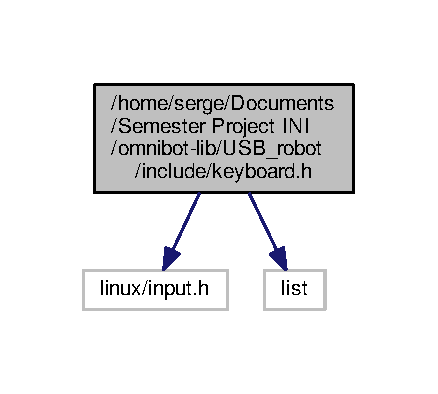
\includegraphics[width=210pt]{keyboard_8h__incl}
\end{center}
\end{figure}
This graph shows which files directly or indirectly include this file\+:\nopagebreak
\begin{figure}[H]
\begin{center}
\leavevmode
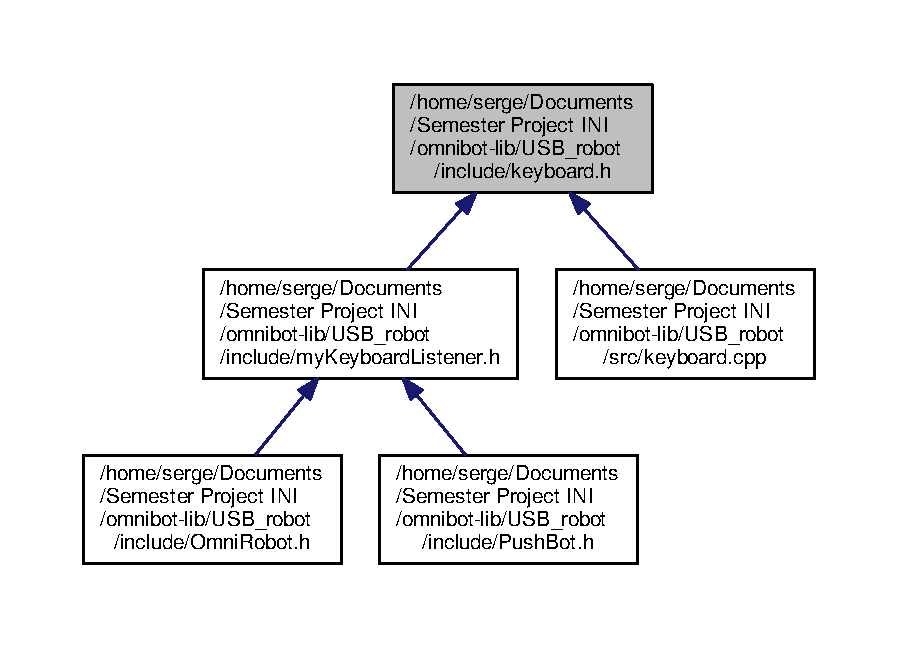
\includegraphics[width=350pt]{keyboard_8h__dep__incl}
\end{center}
\end{figure}
\subsection*{Classes}
\begin{DoxyCompactItemize}
\item 
class \hyperlink{class_keyboard_listener}{Keyboard\+Listener}
\begin{DoxyCompactList}\small\item\em Provides the necessary interface to Listen to keyboard events. \end{DoxyCompactList}\item 
struct \hyperlink{structkeyboard__state}{keyboard\+\_\+state}
\begin{DoxyCompactList}\small\item\em encapsulates the states of all the avaiable keyboard keys \end{DoxyCompactList}\item 
class \hyperlink{classc_keyboard}{c\+Keyboard}
\begin{DoxyCompactList}\small\item\em Manages the communication with an attached keyboard. \end{DoxyCompactList}\end{DoxyCompactItemize}


\subsection{Detailed Description}
This file contains all the necessary interfaces to log keystrokes from the keyboard. One drawback is that all keystrokes are logged, even if the window is not in focus. 


\hypertarget{my_keyboard_listener_8h}{}\section{/home/serge/\+Documents/\+Semester Project I\+N\+I/omnibot-\/lib/\+U\+S\+B\+\_\+robot/include/my\+Keyboard\+Listener.h File Reference}
\label{my_keyboard_listener_8h}\index{/home/serge/\+Documents/\+Semester Project I\+N\+I/omnibot-\/lib/\+U\+S\+B\+\_\+robot/include/my\+Keyboard\+Listener.\+h@{/home/serge/\+Documents/\+Semester Project I\+N\+I/omnibot-\/lib/\+U\+S\+B\+\_\+robot/include/my\+Keyboard\+Listener.\+h}}


This file provides all the functions with respect to the keyboard listener.  


{\ttfamily \#include \char`\"{}keyboard.\+h\char`\"{}}\\*
{\ttfamily \#include \char`\"{}Robot.\+h\char`\"{}}\\*
Include dependency graph for my\+Keyboard\+Listener.\+h\+:\nopagebreak
\begin{figure}[H]
\begin{center}
\leavevmode
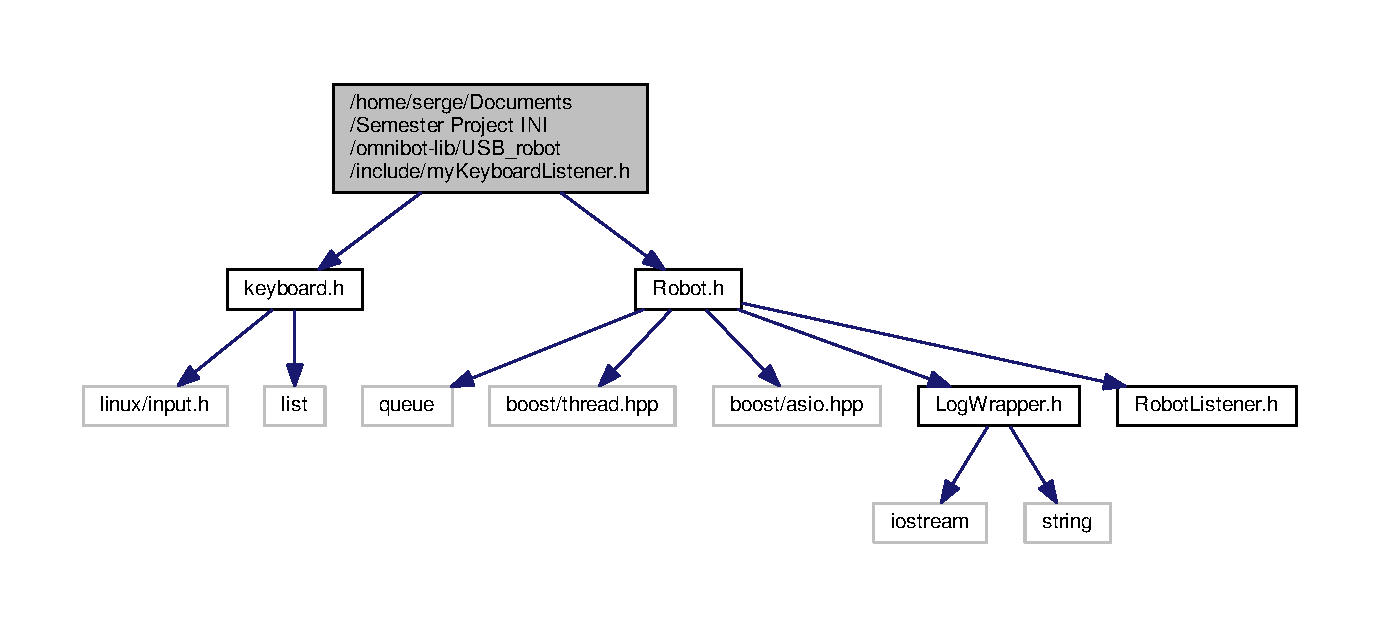
\includegraphics[width=350pt]{my_keyboard_listener_8h__incl}
\end{center}
\end{figure}
This graph shows which files directly or indirectly include this file\+:\nopagebreak
\begin{figure}[H]
\begin{center}
\leavevmode
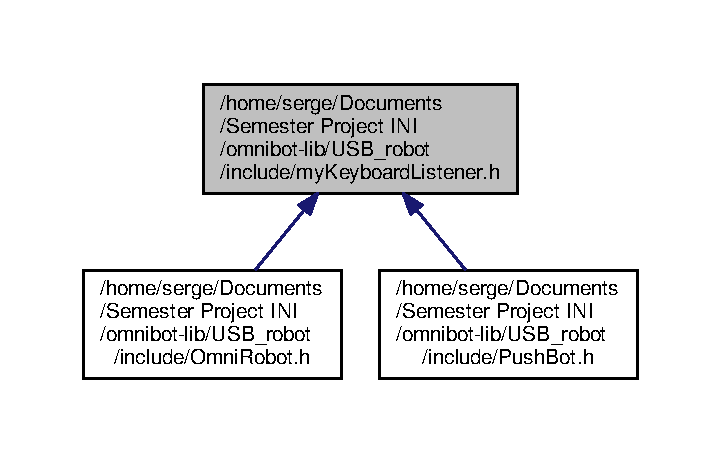
\includegraphics[width=346pt]{my_keyboard_listener_8h__dep__incl}
\end{center}
\end{figure}
\subsection*{Classes}
\begin{DoxyCompactItemize}
\item 
struct \hyperlink{structrobot_drive_parameters}{robot\+Drive\+Parameters}
\item 
class \hyperlink{classmy_keyboard_listener}{my\+Keyboard\+Listener}
\end{DoxyCompactItemize}
\subsection*{Enumerations}
\begin{DoxyCompactItemize}
\item 
enum \hyperlink{my_keyboard_listener_8h_a697eda8a48b6c3569bfda3fc77945a91}{bit\+Shifts} \{ \\*
{\bfseries W\+\_\+\+S\+H\+I\+F\+T} = 0, 
{\bfseries S\+\_\+\+S\+H\+I\+F\+T} = 1, 
{\bfseries A\+\_\+\+S\+H\+I\+F\+T} = 2, 
{\bfseries D\+\_\+\+S\+H\+I\+F\+T} = 3, 
\\*
{\bfseries Q\+\_\+\+S\+H\+I\+F\+T} = 4, 
{\bfseries E\+\_\+\+S\+H\+I\+F\+T} = 5
 \}
\begin{DoxyCompactList}\small\item\em Mapping of the keystrokes. \end{DoxyCompactList}\item 
\hypertarget{my_keyboard_listener_8h_ac18678639755b05ef7e572de6a55c70b}{}enum \hyperlink{my_keyboard_listener_8h_ac18678639755b05ef7e572de6a55c70b}{mapped\+Keys} \{ \\*
{\bfseries \+\_\+\+K\+E\+Y\+\_\+\+W} = (1 $<$$<$ W\+\_\+\+S\+H\+I\+F\+T), 
{\bfseries \+\_\+\+K\+E\+Y\+\_\+\+S} = (1 $<$$<$ S\+\_\+\+S\+H\+I\+F\+T), 
{\bfseries \+\_\+\+K\+E\+Y\+\_\+\+A} = (1 $<$$<$ A\+\_\+\+S\+H\+I\+F\+T), 
{\bfseries \+\_\+\+K\+E\+Y\+\_\+\+D} = (1 $<$$<$ D\+\_\+\+S\+H\+I\+F\+T), 
\\*
{\bfseries \+\_\+\+K\+E\+Y\+\_\+\+E} = (1 $<$$<$ E\+\_\+\+S\+H\+I\+F\+T), 
{\bfseries \+\_\+\+K\+E\+Y\+\_\+\+Q} = (1 $<$$<$ Q\+\_\+\+S\+H\+I\+F\+T)
 \}\label{my_keyboard_listener_8h_ac18678639755b05ef7e572de6a55c70b}

\begin{DoxyCompactList}\small\item\em Mapping of the keystrokes to a more readably form. \end{DoxyCompactList}\item 
\hypertarget{my_keyboard_listener_8h_a51cab4a82059c7fcbbd0baaff4b9901f}{}enum \hyperlink{my_keyboard_listener_8h_a51cab4a82059c7fcbbd0baaff4b9901f}{robot\+Directives} \{ \\*
{\bfseries S\+T\+O\+P} = 0, 
{\bfseries F\+O\+R\+W\+A\+R\+D} = \+\_\+\+K\+E\+Y\+\_\+\+W, 
{\bfseries B\+A\+C\+K\+W\+A\+R\+D} = \+\_\+\+K\+E\+Y\+\_\+\+S, 
{\bfseries L\+E\+F\+T} = \+\_\+\+K\+E\+Y\+\_\+\+A, 
\\*
{\bfseries R\+I\+G\+H\+T} = \+\_\+\+K\+E\+Y\+\_\+\+D, 
{\bfseries T\+U\+R\+N\+\_\+\+C\+C\+W} = \+\_\+\+K\+E\+Y\+\_\+\+Q, 
{\bfseries T\+U\+R\+N\+\_\+\+C\+W} = \+\_\+\+K\+E\+Y\+\_\+\+E, 
{\bfseries F\+W\+R\+\_\+\+A\+R\+C\+\_\+\+R\+I\+G\+H\+T} = \+\_\+\+K\+E\+Y\+\_\+\+W + \+\_\+\+K\+E\+Y\+\_\+\+D, 
\\*
{\bfseries F\+W\+R\+\_\+\+A\+R\+C\+\_\+\+L\+E\+F\+T} = \+\_\+\+K\+E\+Y\+\_\+\+W + \+\_\+\+K\+E\+Y\+\_\+\+A, 
{\bfseries B\+W\+R\+\_\+\+A\+R\+C\+\_\+\+R\+I\+G\+H\+T} = \+\_\+\+K\+E\+Y\+\_\+\+S + \+\_\+\+K\+E\+Y\+\_\+\+D, 
{\bfseries B\+W\+R\+\_\+\+A\+R\+C\+\_\+\+L\+E\+F\+T} = \+\_\+\+K\+E\+Y\+\_\+\+S + \+\_\+\+K\+E\+Y\+\_\+\+A
 \}\label{my_keyboard_listener_8h_a51cab4a82059c7fcbbd0baaff4b9901f}

\begin{DoxyCompactList}\small\item\em Mapping of the keystrokes to drive directives for the robot. \end{DoxyCompactList}\end{DoxyCompactItemize}


\subsection{Detailed Description}
This file provides all the functions with respect to the keyboard listener. 



\subsection{Enumeration Type Documentation}
\hypertarget{my_keyboard_listener_8h_a697eda8a48b6c3569bfda3fc77945a91}{}\index{my\+Keyboard\+Listener.\+h@{my\+Keyboard\+Listener.\+h}!bit\+Shifts@{bit\+Shifts}}
\index{bit\+Shifts@{bit\+Shifts}!my\+Keyboard\+Listener.\+h@{my\+Keyboard\+Listener.\+h}}
\subsubsection[{bit\+Shifts}]{\setlength{\rightskip}{0pt plus 5cm}enum {\bf bit\+Shifts}}\label{my_keyboard_listener_8h_a697eda8a48b6c3569bfda3fc77945a91}


Mapping of the keystrokes. 

Pressing a key results in setting a bit at the corresponding position in a int variable. This allows filtering keys with no mapping and storing the state of the key and detecting combinations of keys. Key presses map to bit = 1 and key releases to bit=0 at the respective bit position of the corresponding key as defined by bit\+Shifts. \begin{DoxySeeAlso}{See also}
\hyperlink{my_keyboard_listener_8h_ac18678639755b05ef7e572de6a55c70b}{mapped\+Keys} 
\end{DoxySeeAlso}

\hypertarget{my_log_listener_e_d_v_s_8h}{}\section{/home/serge/\+Documents/\+Semester Project I\+N\+I/omnibot-\/lib/\+U\+S\+B\+\_\+robot/include/my\+Log\+Listener\+E\+D\+V\+S.h File Reference}
\label{my_log_listener_e_d_v_s_8h}\index{/home/serge/\+Documents/\+Semester Project I\+N\+I/omnibot-\/lib/\+U\+S\+B\+\_\+robot/include/my\+Log\+Listener\+E\+D\+V\+S.\+h@{/home/serge/\+Documents/\+Semester Project I\+N\+I/omnibot-\/lib/\+U\+S\+B\+\_\+robot/include/my\+Log\+Listener\+E\+D\+V\+S.\+h}}
{\ttfamily \#include \char`\"{}E\+B\+V\+\_\+\+E\+D\+V\+S4337\+Serial\+U\+S\+B.\+h\char`\"{}}\\*
Include dependency graph for my\+Log\+Listener\+E\+D\+V\+S.\+h\+:\nopagebreak
\begin{figure}[H]
\begin{center}
\leavevmode
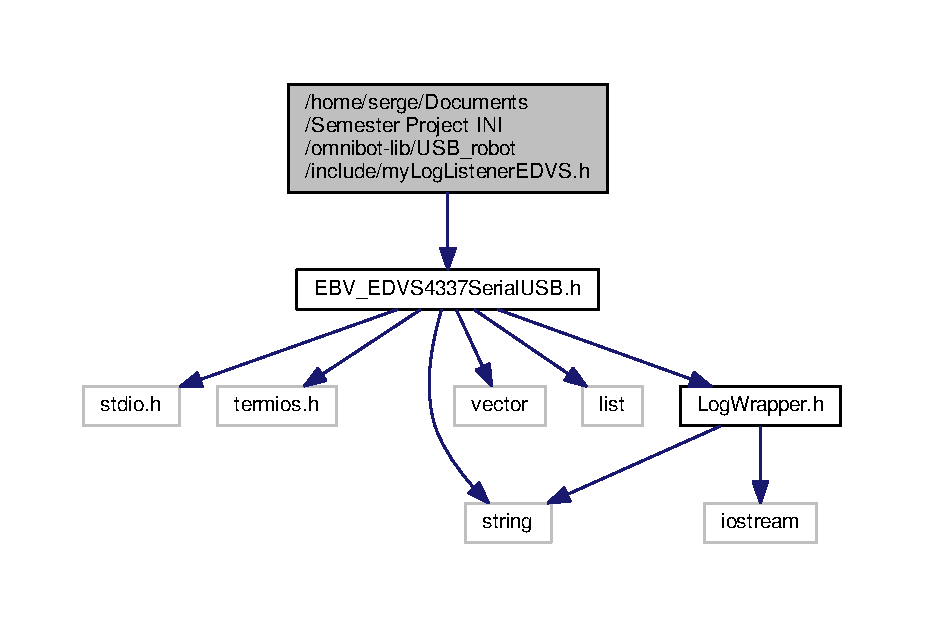
\includegraphics[width=350pt]{my_log_listener_e_d_v_s_8h__incl}
\end{center}
\end{figure}
\subsection*{Classes}
\begin{DoxyCompactItemize}
\item 
class \hyperlink{classmy_log_listener_e_d_v_s}{my\+Log\+Listener\+E\+D\+V\+S}
\begin{DoxyCompactList}\small\item\em This class provides a concrete implementation of a e\+D\+V\+S event listener that logs the received events to a file. \end{DoxyCompactList}\end{DoxyCompactItemize}


\subsection{Detailed Description}
\begin{DoxyAuthor}{Author}
Michel Frising
\end{DoxyAuthor}
This file contains a concrete implementation of a e\+D\+V\+S event listener that writes events in formatted form to a log file. This step may be slow, to increase performance one could switch to a binary stream. If this is still too slow, a ringbuffer has to be implemented where the events are added on one end taken from the other.

\begin{DoxySeeAlso}{See also}
\href{https://en.wikipedia.org/wiki/Circular_buffer}{\tt https\+://en.\+wikipedia.\+org/wiki/\+Circular\+\_\+buffer} 
\end{DoxySeeAlso}

\hypertarget{_omni_robot_8h}{}\section{/home/serge/\+Documents/\+Semester Project I\+N\+I/omnibot-\/lib/\+U\+S\+B\+\_\+robot/include/\+Omni\+Robot.h File Reference}
\label{_omni_robot_8h}\index{/home/serge/\+Documents/\+Semester Project I\+N\+I/omnibot-\/lib/\+U\+S\+B\+\_\+robot/include/\+Omni\+Robot.\+h@{/home/serge/\+Documents/\+Semester Project I\+N\+I/omnibot-\/lib/\+U\+S\+B\+\_\+robot/include/\+Omni\+Robot.\+h}}
{\ttfamily \#include $<$stdio.\+h$>$}\\*
{\ttfamily \#include $<$termios.\+h$>$}\\*
{\ttfamily \#include $<$string$>$}\\*
{\ttfamily \#include $<$vector$>$}\\*
{\ttfamily \#include $<$queue$>$}\\*
{\ttfamily \#include $<$list$>$}\\*
{\ttfamily \#include $<$Robot.\+h$>$}\\*
{\ttfamily \#include $<$my\+Keyboard\+Listener.\+h$>$}\\*
{\ttfamily \#include $<$fstream$>$}\\*
Include dependency graph for Omni\+Robot.\+h\+:\nopagebreak
\begin{figure}[H]
\begin{center}
\leavevmode
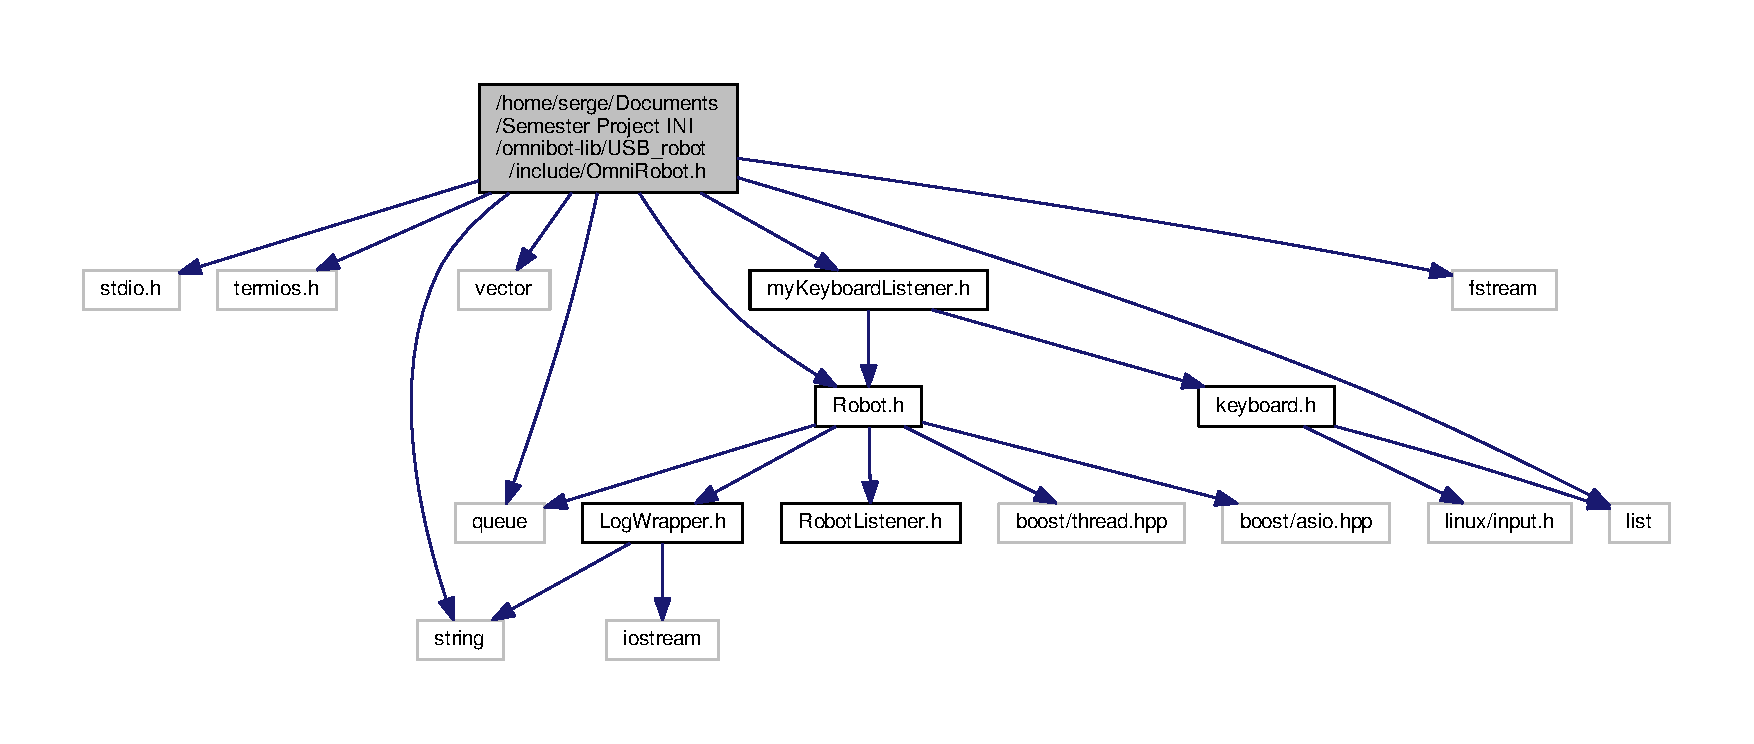
\includegraphics[width=350pt]{_omni_robot_8h__incl}
\end{center}
\end{figure}
\subsection*{Classes}
\begin{DoxyCompactItemize}
\item 
struct \hyperlink{structrobot_drive_state}{robot\+Drive\+State}
\begin{DoxyCompactList}\small\item\em encapsulates the mid-\/level robot drive parameters \end{DoxyCompactList}\item 
class \hyperlink{class_omni_robot}{Omni\+Robot}
\begin{DoxyCompactList}\small\item\em Interface to the Omni\+Rob from N\+S\+T. \end{DoxyCompactList}\end{DoxyCompactItemize}


\subsection{Detailed Description}
\begin{DoxyAuthor}{Author}
Michel Frising
\end{DoxyAuthor}
This file provides the necessary interfaces for driving the N\+S\+T Omni\+Rob 
\hypertarget{_push_bot_8h}{}\section{/home/serge/\+Documents/\+Semester Project I\+N\+I/omnibot-\/lib/\+U\+S\+B\+\_\+robot/include/\+Push\+Bot.h File Reference}
\label{_push_bot_8h}\index{/home/serge/\+Documents/\+Semester Project I\+N\+I/omnibot-\/lib/\+U\+S\+B\+\_\+robot/include/\+Push\+Bot.\+h@{/home/serge/\+Documents/\+Semester Project I\+N\+I/omnibot-\/lib/\+U\+S\+B\+\_\+robot/include/\+Push\+Bot.\+h}}
{\ttfamily \#include $<$stdio.\+h$>$}\\*
{\ttfamily \#include $<$termios.\+h$>$}\\*
{\ttfamily \#include $<$string$>$}\\*
{\ttfamily \#include $<$vector$>$}\\*
{\ttfamily \#include $<$queue$>$}\\*
{\ttfamily \#include $<$list$>$}\\*
{\ttfamily \#include $<$Robot.\+h$>$}\\*
{\ttfamily \#include $<$my\+Keyboard\+Listener.\+h$>$}\\*
Include dependency graph for Push\+Bot.\+h\+:\nopagebreak
\begin{figure}[H]
\begin{center}
\leavevmode
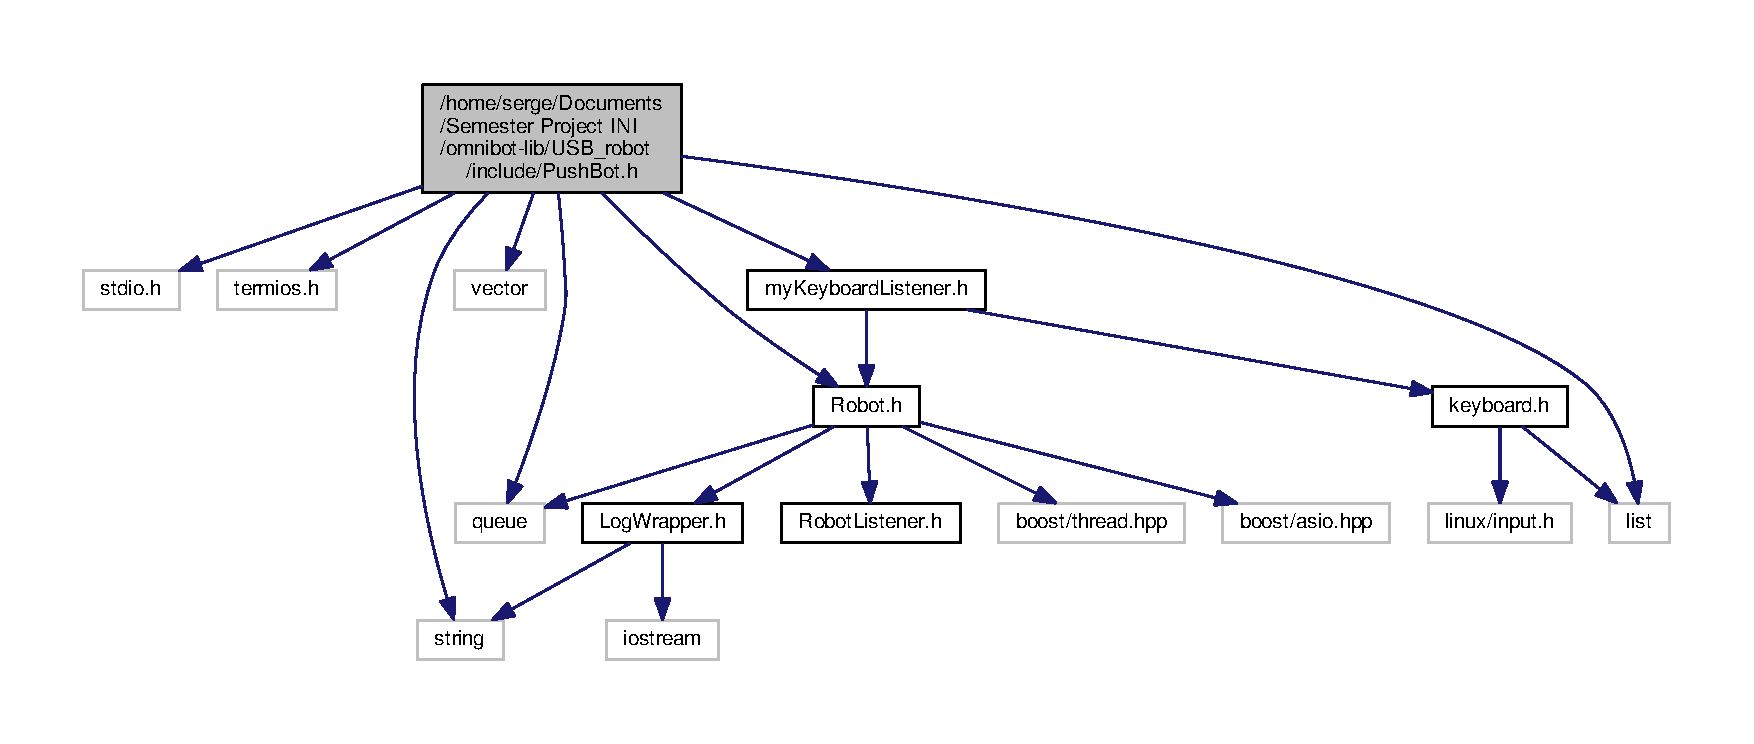
\includegraphics[width=350pt]{_push_bot_8h__incl}
\end{center}
\end{figure}
\subsection*{Classes}
\begin{DoxyCompactItemize}
\item 
class \hyperlink{class_push_bot}{Push\+Bot}
\begin{DoxyCompactList}\small\item\em Mid-\/\+Level interface to the \hyperlink{class_push_bot}{Push\+Bot}. Communnication via Wi\+Fi. \end{DoxyCompactList}\end{DoxyCompactItemize}
\subsection*{Macros}
\begin{DoxyCompactItemize}
\item 
\hypertarget{_push_bot_8h_af1abcb51a4aa27a5a5a7958c03448134}{}\#define {\bfseries M\+A\+X\+\_\+\+C\+O\+M\+M\+A\+N\+D\+\_\+\+L\+E\+N\+G\+T\+H}~50\label{_push_bot_8h_af1abcb51a4aa27a5a5a7958c03448134}

\item 
\hypertarget{_push_bot_8h_aac3553b3932cbfeeac4526ce7ca0336b}{}\#define {\bfseries S\+P\+E\+E\+D}~20\label{_push_bot_8h_aac3553b3932cbfeeac4526ce7ca0336b}

\end{DoxyCompactItemize}


\subsection{Detailed Description}
protoptypes for the Omni\+Rob U\+S\+B communiaction and low-\/level commands 
\hypertarget{_robot_listener_8h}{}\section{/home/serge/\+Documents/\+Semester Project I\+N\+I/omnibot-\/lib/\+U\+S\+B\+\_\+robot/include/\+Robot\+Listener.h File Reference}
\label{_robot_listener_8h}\index{/home/serge/\+Documents/\+Semester Project I\+N\+I/omnibot-\/lib/\+U\+S\+B\+\_\+robot/include/\+Robot\+Listener.\+h@{/home/serge/\+Documents/\+Semester Project I\+N\+I/omnibot-\/lib/\+U\+S\+B\+\_\+robot/include/\+Robot\+Listener.\+h}}
This graph shows which files directly or indirectly include this file\+:\nopagebreak
\begin{figure}[H]
\begin{center}
\leavevmode
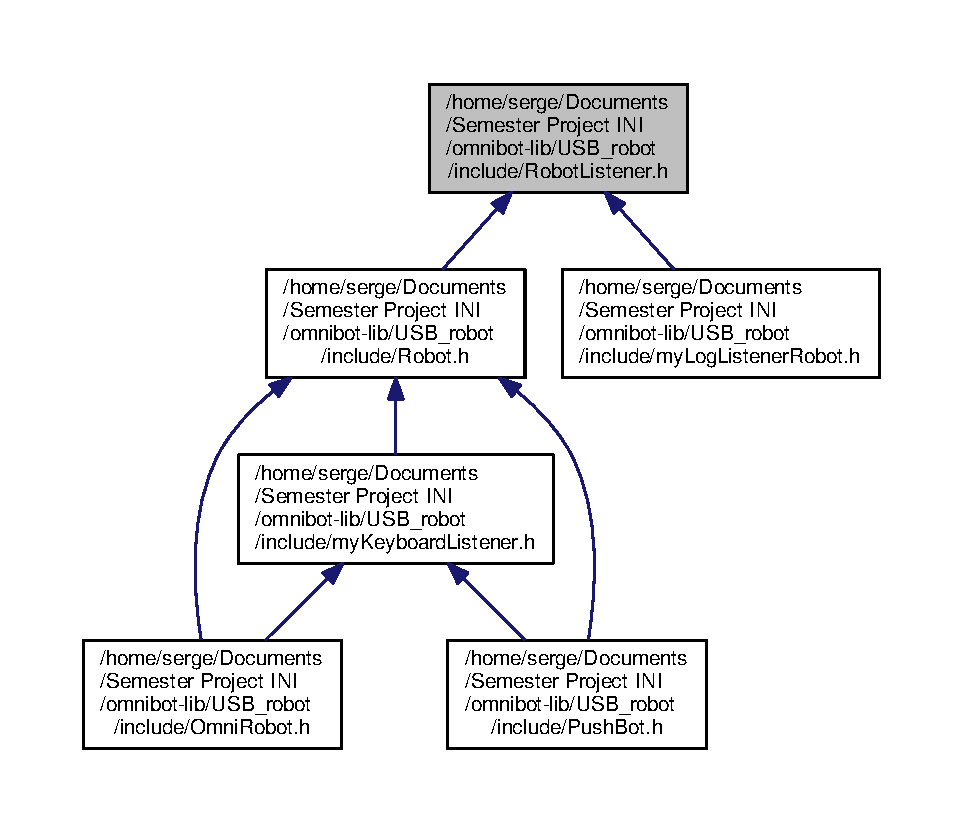
\includegraphics[width=350pt]{_robot_listener_8h__dep__incl}
\end{center}
\end{figure}
\subsection*{Classes}
\begin{DoxyCompactItemize}
\item 
struct \hyperlink{structservo_signals}{servo\+Signals}
\item 
struct \hyperlink{structbumper}{bumper}
\item 
class \hyperlink{class_robot_listener}{Robot\+Listener}
\begin{DoxyCompactList}\small\item\em Abstarct base class providing the necessary interface to observe the servo states and bumper states of the observed robot. \end{DoxyCompactList}\end{DoxyCompactItemize}


\subsection{Detailed Description}
\begin{DoxyAuthor}{Author}
Michel Frising Provides a concrete implementation of the abstract \hyperlink{class_robot_listener}{Robot\+Listener} to receive the servo states and the bumber states parsed from the robot event stream. At the moment all loging capabilities are commented out, but Prof. Conradth from N\+S\+T in Munich announced that in a feature release of the Omni\+Rob firmware broadcasting capabilities, such as the e\+D\+V\+S event stream will be implemented, where this class will come in handy.

Michel Frising Provides an abstract base class to receive the servo states and the bumber states parsed from the robot event stream. 
\end{DoxyAuthor}

\hypertarget{_t_c_p_connector_8h}{}\section{/home/serge/\+Documents/\+Semester Project I\+N\+I/omnibot-\/lib/\+U\+S\+B\+\_\+robot/include/\+T\+C\+P\+Connector.h File Reference}
\label{_t_c_p_connector_8h}\index{/home/serge/\+Documents/\+Semester Project I\+N\+I/omnibot-\/lib/\+U\+S\+B\+\_\+robot/include/\+T\+C\+P\+Connector.\+h@{/home/serge/\+Documents/\+Semester Project I\+N\+I/omnibot-\/lib/\+U\+S\+B\+\_\+robot/include/\+T\+C\+P\+Connector.\+h}}


All the functions managing communications over T\+C\+P/\+I\+P are defined here.  


\subsection*{Functions}
\begin{DoxyCompactItemize}
\item 
int \hyperlink{_t_c_p_connector_8h_a29b7caffa5e8a2a25691b19d7cd8204a}{get\+T\+C\+P\+File\+Descriptor} (const char $\ast$hostname, unsigned int portno)
\begin{DoxyCompactList}\small\item\em Opens a file descriptor to a T\+C\+P socket. \end{DoxyCompactList}\end{DoxyCompactItemize}


\subsection{Detailed Description}
All the functions managing communications over T\+C\+P/\+I\+P are defined here. 



\subsection{Function Documentation}
\hypertarget{_t_c_p_connector_8h_a29b7caffa5e8a2a25691b19d7cd8204a}{}\index{T\+C\+P\+Connector.\+h@{T\+C\+P\+Connector.\+h}!get\+T\+C\+P\+File\+Descriptor@{get\+T\+C\+P\+File\+Descriptor}}
\index{get\+T\+C\+P\+File\+Descriptor@{get\+T\+C\+P\+File\+Descriptor}!T\+C\+P\+Connector.\+h@{T\+C\+P\+Connector.\+h}}
\subsubsection[{get\+T\+C\+P\+File\+Descriptor}]{\setlength{\rightskip}{0pt plus 5cm}int get\+T\+C\+P\+File\+Descriptor (
\begin{DoxyParamCaption}
\item[{const char $\ast$}]{hostname, }
\item[{unsigned int}]{portno}
\end{DoxyParamCaption}
)}\label{_t_c_p_connector_8h_a29b7caffa5e8a2a25691b19d7cd8204a}


Opens a file descriptor to a T\+C\+P socket. 


\begin{DoxyParams}{Parameters}
{\em hostname} & The name of the device we want to connect to (I\+P addess for example) \\
\hline
{\em portno} & Number of the port we want to connect to. \\
\hline
\end{DoxyParams}
\begin{DoxyReturn}{Returns}
if successful, a File Descriptor to the opened devive, else -\/1. 
\end{DoxyReturn}

\hypertarget{_u_s_b_connector_8h}{}\section{/home/serge/\+Documents/\+Semester Project I\+N\+I/omnibot-\/lib/\+U\+S\+B\+\_\+robot/include/\+U\+S\+B\+Connector.h File Reference}
\label{_u_s_b_connector_8h}\index{/home/serge/\+Documents/\+Semester Project I\+N\+I/omnibot-\/lib/\+U\+S\+B\+\_\+robot/include/\+U\+S\+B\+Connector.\+h@{/home/serge/\+Documents/\+Semester Project I\+N\+I/omnibot-\/lib/\+U\+S\+B\+\_\+robot/include/\+U\+S\+B\+Connector.\+h}}


This file provides all the necessary functions to open a serial port to a U\+S\+B connected device.  


{\ttfamily \#include $<$linux/serial.\+h$>$}\\*
{\ttfamily \#include $<$termio.\+h$>$}\\*
{\ttfamily \#include $<$Log\+Wrapper.\+h$>$}\\*
Include dependency graph for U\+S\+B\+Connector.\+h\+:\nopagebreak
\begin{figure}[H]
\begin{center}
\leavevmode
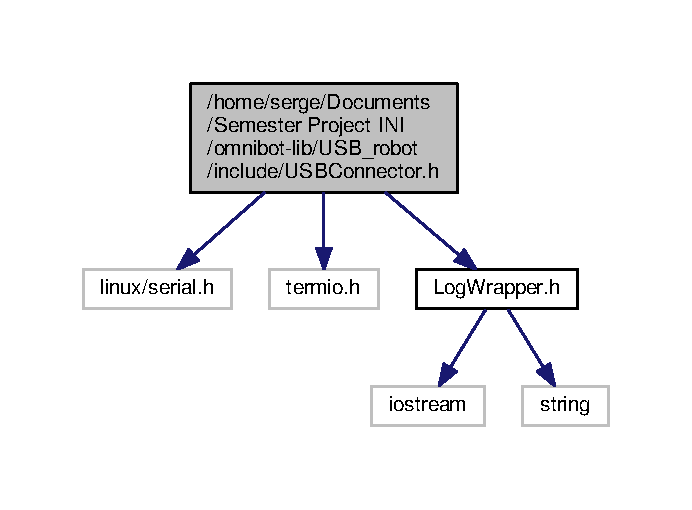
\includegraphics[width=332pt]{_u_s_b_connector_8h__incl}
\end{center}
\end{figure}
\subsection*{Functions}
\begin{DoxyCompactItemize}
\item 
int \hyperlink{_u_s_b_connector_8h_a1762dd5ceb7cca8e14e100486f1681e4}{get\+U\+S\+B\+File\+Descriptor} (char const $\ast$port\+\_\+name=\char`\"{}/dev/tty\+U\+S\+B0\char`\"{}, unsigned int arg\+\_\+baudrate=2000000, std\+::string dev\+Name=\char`\"{}Device\char`\"{})
\begin{DoxyCompactList}\small\item\em Opens and configures the serial port. \end{DoxyCompactList}\end{DoxyCompactItemize}


\subsection{Detailed Description}
This file provides all the necessary functions to open a serial port to a U\+S\+B connected device. 

This is possible because the camera an robot are fitted with an F\+T\+D\+I chip. 

\subsection{Function Documentation}
\hypertarget{_u_s_b_connector_8h_a1762dd5ceb7cca8e14e100486f1681e4}{}\index{U\+S\+B\+Connector.\+h@{U\+S\+B\+Connector.\+h}!get\+U\+S\+B\+File\+Descriptor@{get\+U\+S\+B\+File\+Descriptor}}
\index{get\+U\+S\+B\+File\+Descriptor@{get\+U\+S\+B\+File\+Descriptor}!U\+S\+B\+Connector.\+h@{U\+S\+B\+Connector.\+h}}
\subsubsection[{get\+U\+S\+B\+File\+Descriptor}]{\setlength{\rightskip}{0pt plus 5cm}int get\+U\+S\+B\+File\+Descriptor (
\begin{DoxyParamCaption}
\item[{char const $\ast$}]{port\+\_\+name = {\ttfamily \char`\"{}/dev/ttyUSB0\char`\"{}}, }
\item[{unsigned int}]{arg\+\_\+baudrate = {\ttfamily 2000000}, }
\item[{std\+::string}]{dev\+Name = {\ttfamily \char`\"{}Device\char`\"{}}}
\end{DoxyParamCaption}
)}\label{_u_s_b_connector_8h_a1762dd5ceb7cca8e14e100486f1681e4}


Opens and configures the serial port. 

The requested device is opened with read and write enabled. The requested baudrate is set and the serial port configured to be in raw mode, non-\/blocking and with hardware control enabled. For more information see also here\+: \begin{DoxySeeAlso}{See also}
\href{http://inilabs.com/support/hardware/edvs/#h.2v48aal08cim}{\tt http\+://inilabs.\+com/support/hardware/edvs/\#h.\+2v48aal08cim} 
\end{DoxySeeAlso}

\begin{DoxyParams}{Parameters}
{\em port\+\_\+name} & the name of the port is device is connected to, as listed under \textquotesingle{}ls /dev/\textquotesingle{} \\
\hline
{\em arg\+\_\+baudrate} & the requested communication baudrate \\
\hline
\end{DoxyParams}
\begin{DoxyReturn}{Returns}
if successful return a valid file descriptr to the port, else -\/1. 
\end{DoxyReturn}

\hypertarget{keyboard_8cpp}{}\section{/home/serge/\+Documents/\+Semester Project I\+N\+I/omnibot-\/lib/\+U\+S\+B\+\_\+robot/src/keyboard.cpp File Reference}
\label{keyboard_8cpp}\index{/home/serge/\+Documents/\+Semester Project I\+N\+I/omnibot-\/lib/\+U\+S\+B\+\_\+robot/src/keyboard.\+cpp@{/home/serge/\+Documents/\+Semester Project I\+N\+I/omnibot-\/lib/\+U\+S\+B\+\_\+robot/src/keyboard.\+cpp}}


This file provides the implementation of the keyboard communication.  


{\ttfamily \#include $<$iostream$>$}\\*
{\ttfamily \#include $<$fcntl.\+h$>$}\\*
{\ttfamily \#include $<$pthread.\+h$>$}\\*
{\ttfamily \#include $<$linux/input.\+h$>$}\\*
{\ttfamily \#include $<$unistd.\+h$>$}\\*
{\ttfamily \#include $<$list$>$}\\*
{\ttfamily \#include $<$errno.\+h$>$}\\*
{\ttfamily \#include $<$stdlib.\+h$>$}\\*
{\ttfamily \#include $<$stdio.\+h$>$}\\*
{\ttfamily \#include $<$cstring$>$}\\*
{\ttfamily \#include $<$termios.\+h$>$}\\*
{\ttfamily \#include $<$dirent.\+h$>$}\\*
{\ttfamily \#include \char`\"{}keyboard.\+h\char`\"{}}\\*
Include dependency graph for keyboard.\+cpp\+:\nopagebreak
\begin{figure}[H]
\begin{center}
\leavevmode
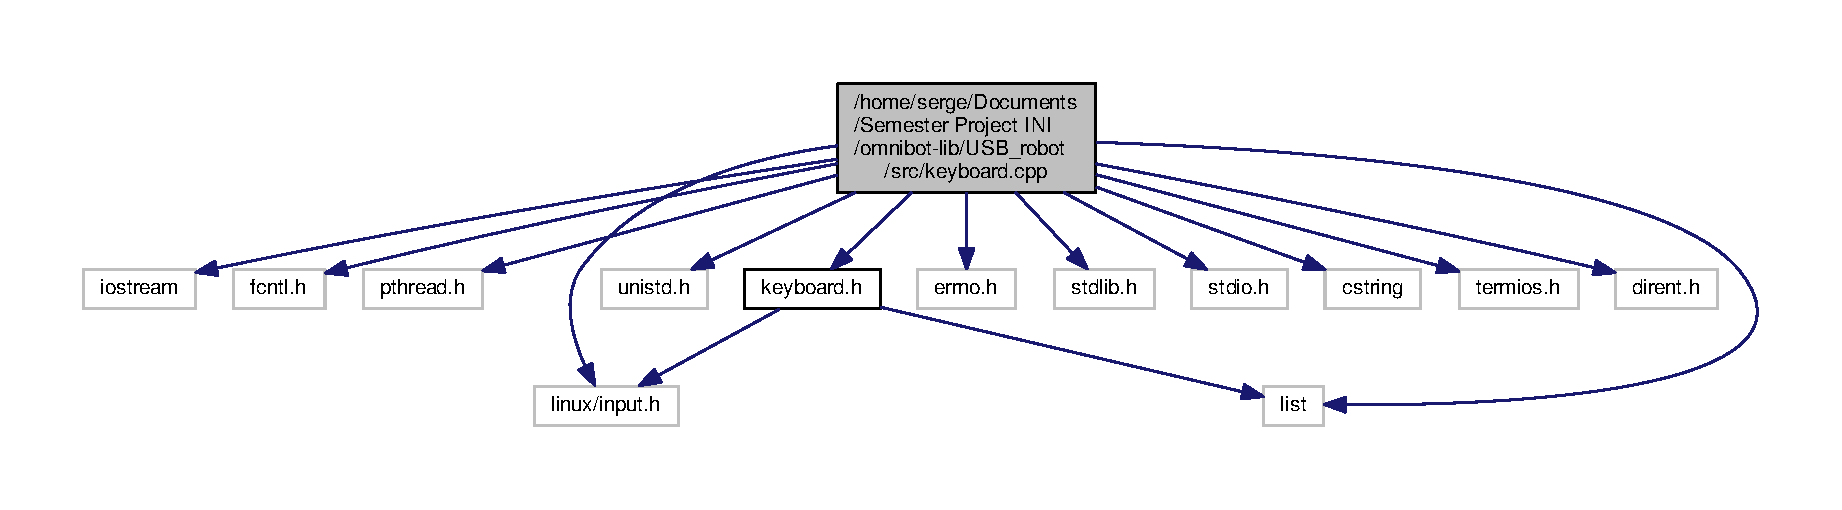
\includegraphics[width=350pt]{keyboard_8cpp__incl}
\end{center}
\end{figure}
\subsection*{Functions}
\begin{DoxyCompactItemize}
\item 
void \hyperlink{keyboard_8cpp_ab44bf9d3158f256a1002b4d655c5d920}{init\+Termios} (int echo)
\begin{DoxyCompactList}\small\item\em Store old Terminal settings and Initialize new terminal i/o settings. \end{DoxyCompactList}\item 
\hypertarget{keyboard_8cpp_a6de63f92240376d8f02045667c9c86ed}{}void \hyperlink{keyboard_8cpp_a6de63f92240376d8f02045667c9c86ed}{reset\+Termios} ()\label{keyboard_8cpp_a6de63f92240376d8f02045667c9c86ed}

\begin{DoxyCompactList}\small\item\em Restore old terminal i/o settings. \end{DoxyCompactList}\item 
\hypertarget{keyboard_8cpp_a9855a68540bc44e456ede87540ba9320}{}bool {\bfseries has\+Ending} (std\+::string const \&full\+String, std\+::string const \&ending)\label{keyboard_8cpp_a9855a68540bc44e456ede87540ba9320}

\item 
\hypertarget{keyboard_8cpp_ad18ddfac04f93ff317f59fe3325208a5}{}std\+::string {\bfseries find\+Keyboard} ()\label{keyboard_8cpp_ad18ddfac04f93ff317f59fe3325208a5}

\end{DoxyCompactItemize}


\subsection{Detailed Description}
This file provides the implementation of the keyboard communication. 



\subsection{Function Documentation}
\hypertarget{keyboard_8cpp_ab44bf9d3158f256a1002b4d655c5d920}{}\index{keyboard.\+cpp@{keyboard.\+cpp}!init\+Termios@{init\+Termios}}
\index{init\+Termios@{init\+Termios}!keyboard.\+cpp@{keyboard.\+cpp}}
\subsubsection[{init\+Termios}]{\setlength{\rightskip}{0pt plus 5cm}void init\+Termios (
\begin{DoxyParamCaption}
\item[{int}]{echo}
\end{DoxyParamCaption}
)}\label{keyboard_8cpp_ab44bf9d3158f256a1002b4d655c5d920}


Store old Terminal settings and Initialize new terminal i/o settings. 


\begin{DoxyParams}{Parameters}
{\em echo} & turns the terminal echo mode on (1) or off (0). \\
\hline
\end{DoxyParams}

%--- End generated contents ---

% Index
\backmatter
\newpage
\phantomsection
\clearemptydoublepage
\addcontentsline{toc}{chapter}{Index}
\printindex

\end{document}
